\label{aqft}
\begin{chapterbox}
\vspace{-60pt}
\chapter{Advanced Quantum Field Theory}
\vspace{-30pt}
\centering\normalsize\textit{Lent Term 2018 - Dr D. Skinner}
\end{chapterbox}
\vspace{20pt}
%\begin{multicols*}{2}
\minitoc
\newpage
\section{Introduction}
What is a quantum field theory (QFT)? Simply it's the quantum version of a field theory, but it's also a mathematical tool useful for studying ideas outside the direct scope.\footnote{For example knot invariants, Calabi-Yau manifolds etc.} What do we have to do to design a QFT?
\begin{enumerate}
\item First we have to choose the space on which it lives. Often this is a (pseudo)-Riemannian manifold, $(\mM, g)$, but this may depend on the scenario;
\begin{itemize}
\item Particle physics: $(\mM, g) = (\RR^4, \delta) \,\,\text{or}\,\,(\RR^{3,1}, \eta)$
\item Condensed matter: $(\mM, g) = (\RR^3, \delta)$
\item Cosmology: $(\mM, g) = (\RR^{3,1}, g_{\text{FRW}})$
\item String Theory: $(\mM, g) = \left(\Sigma, [g] = \set{g \sim e^{2\phi(x)}g}\right)$ where $\Sigma$ is a Riemann surface.
\end{itemize}
\item Next we have to choose the fields. In the simplest case these are just scalar fields\index{field!scalar}, which are functions $\phi : \mM \rightarrow \RR, \CC$. However, there are lots of other options;
\begin{itemize}
\item Consider $\phi^a : \mM \rightarrow \mathcal{N}$, where $(\mathcal{N}, g)$ is another Riemannian manifold e.g. $\phi : \RR^4 \rightarrow G / H$ which is the case for pions\index{pions} in the SM.
\item Gauge theories: fields are $A_{\mu}$, or connections on $P \rightarrow \mM$
\item Charged matter: sections of a vector bundle $E \rightarrow \mM$
\item Spinor fields, $\psi$
\end{itemize}
In general we let $\mC$ denote the space of all field configurations on $\mM$ so $\phi \in \mC$ represents a picture of what the field looks like.
\item Finally, we need to choose an action $S\left[\phi\right]$, where $S : \mC \rightarrow \RR$, a function on the space of fields. The \emph{critical points}\index{critical point} of this action\footnote{$\phi_0 \in \mC$ such that $\delta S\left[\phi_0\right] = 0$} correspond to field configurations that satisfy the classical equations of motion. We usually choose the action to be local. This means it involves only one integral over the underlying space $\mM$.\footnotemark
\begin{equation}
S\left[\phi\right] = \int_{\mM}{\mL(\phi, \del_\mu \phi)\sqrt{-g}\upd{^d x}}
\end{equation}
\end{enumerate}
\footnotetext{
This is actually a very strong condition on the action. Even a monomial on $\mC$ looks like;
\begin{equation*}
\Lambda\left[\phi\right] = \int_{\mM^{\otimes n}}{\ud^d x_1\cdots \upd{^d x_n}\phi(x_1)\cdots\phi(x_n)\Lambda(x_1, \ldots x_n)}
\end{equation*}
Locality ensures we take $\Lambda(x_1, \ldots, x_n) = \lambda(x_1)\delta(x_1 - x_2)\cdots\delta(x_{n-1} - x_n)$, so that;
\begin{equation*}
\Lambda\left[\phi\right] = \int_{\mM}{\upd{^d x}\lambda(x)\phi^n(x)}
\end{equation*}
We often take $\lambda(x)$ to be constant, a \emph{coupling constant}\index{coupling constant}, but we will see that QFT forces us to consider the more general case.
}
So having made these choices, what do we actually measure? The main interest is the path integral\index{path integral};
\begin{equation}
\int_{\mC}{\mD \phi \,\, e^{-\tfrac{S\left[\phi\right]}{\hbar}}} \qquad \text{or} \qquad \int_{\mC}{\mD \phi \,\, e^{i\tfrac{S\left[\phi\right]}{\hbar}}} \text{ if} \mM \text{ is Lorentzian}
\end{equation}
We start to evaluate this qualitatively. It is an integral over an infinite dimensional space with weighting functions $\exp(-S[\phi]/\hbar)$, which tries to suppress wild field configurations.\footnote{For example, $\del \phi$ is large when $\phi$ oscillates rapidly, or $\phi$ large if the field value is large leading to large $S[\phi]$ and small $\exp(-S[\phi]/\hbar)$.} But, as in statistical mechanics, there is an energy vs entropy competition between suppressing wild configurations, and the fact that there are simply many more of them compared to `sensible' field profiles. There is a very delicate balance between the two as to whether the path integral will converge. The partition function\index{partition function} for $\mM$ compact and without boundary;
\begin{equation}
\mathcal{Z} = \int_{\mC[\mM]}{\mD \phi e^{-\tfrac{S[\phi]}{\hbar}}} = \mathcal{Z}_{(\mM, g)}(\lambda, \ldots)
\end{equation}
We also want to compute correlation functions\index{correlation function}. This involves picking other functions $\mO^i[\phi]$, known as operators\index{operator} or operator insertions\index{operator!insertions} and define;
\begin{equation}
\left< \prod_i {\mO^i[\phi]} \right> = \frac{1}{\mathcal{Z}}\int_{\mC}{\mD \phi \,\, e^{-S[\phi]/\hbar}\prod_i{\mO^i[\phi]}}
\end{equation}
Operator insertions can live at points $x_i \in \mM$ or integrated over some subspace of $\mM$ e.g. a Wilson loop. These correlation functions depend on all the choices we made for our QFT as well as the $\mO[\phi]$. But they don't depend on the fields; these were integrated out.

\paraskip
Correlation functions\index{correlation functions} are also closely related to the partition function. Suppose $S[\phi]$ contains a term $\lambda \int_{\mM}{\ud^d x\sqrt{-g}\phi^4}$, then (assuming we can move the derivative through $\mathcal{D} \phi$);
\begin{align*}
-\hbar \frac{\del}{\del \lambda}\mZ &= -\hbar \int{\mD\phi \,\,\frac{\del}{\del \lambda}e^{-S[\phi]/\hbar}} \\
&=\int{\mD\phi \,\, e^{-S[\phi]/\hbar}\int_{\mM}{\upd{^d x}\sqrt{-g}\phi^4}} \\
\Rightarrow -\frac{\hbar}{\mZ}\frac{\del \mZ}{\del \lambda} &= \left< \int_{\mM}{\sqrt{-g}\upd{^d x}\phi^4} \right>
\end{align*}
So we see knowing $Z_{(\mM, g)}(\lambda, \ldots)$ is equivalent to knowing the correlation functions of terms in the action. Let's extend this to correlators of operators that depend on $\phi$ only at a point, e.g. $\phi(x)^2$. Now we modify the action to allow it to contain sources for these operators;\footnote{Compare the $J_i(x)$ in this expression to the most general $\lambda(x)$ we obtained by imposing locality.}
\begin{equation}
S[\phi] \mapsto S[\phi] + \sum_{i}{\int_{\mM}{\upd{^d x} J_i(x)\mO_i(x)}}
\end{equation}
Then we find, using $\delta J(y)/\delta J(x) = \delta(x - y)$;
\begin{align*}
\left.-\hbar\frac{\delta \mZ}{\delta J(x)}\right|_{J = 0} &= \left.-\hbar\int{\mD\phi\,\,\frac{\delta}{\delta J(x)}\exp\left[\left(-S[\phi] - \int{\upd{^d y}J(y)\mO(y)}\right)/\hbar\right]}\right|_{J = 0} \\
&= \int{\mD\phi e^{-S[\phi]/\hbar}\int{\upd{^d y}\frac{\delta J(y)}{\delta J(x)}\mO(y)}} \\
\Rightarrow \left.-\frac{\hbar}{\mZ}\frac{\delta \mZ}{\delta J(x)}\right|_{J=0} &= \int{\mD\phi e^{-S[\phi]/\hbar}\mO(x)} = \left< \mO(x) \right>
\end{align*}
More generally;
\begin{equation}
-\left.\frac{\hbar}{\mZ}\frac{\delta^n \mZ[J_i]}{\delta J_1(x_1)\cdots \delta J_n(x_n)}\right|_{J_i = 0} = \left< \mO_1(x_1)\cdots\mO_n(x_n) \right>
\end{equation}
The standard example of this is for $\mO(x) = \phi(x)$ so that the source term is $\int_{\mM}{\upd{^d x}J(x)\phi(x)}$. 
\subsection{Boundaries and Hilbert Spaces}
Suppose now that $\mM$ has a boundary $\bigcup_i B_i$. Then to compute a path integral with $\del \mM \neq \varnothing$, we have to specify boundary conditions on the fields. These are associated with a Hilbert space\index{Hilbert space} of the QFT. Then;
\begin{equation}
\int_{\left.\phi\right|_{B_i} = \phi_i}{\mD\phi\,\, e^{-S[\phi]/\hbar}}
\end{equation}
must depend on $\phi_i$ on each component of the boundary. The standard example to choose is $\mM = \mathcal{N}\times I$ where $\mathcal{N}$ is a $(d-1)$-dimensional manifold and $I = \left[0, T\right]$. We have a Hilbert space, $\mathfrak{H}$ on $\mathcal{N}_{t = 0}$ and $\mathcal{N}_{t = T}$, as well as an associated outward normal vector, $n^\mu_{0, 1}$. By construction, these naturally have opposite orientations on the space. Then the path integral can be thought of as a map;
\begin{equation}
U(T) : \mathfrak{H} \rightarrow \mathfrak{H}
\end{equation}
or in other words;
\begin{equation}
\bra{\phi_{1}}U(T)\ket{\phi_0} = \int_{\left.\phi\right|_{\mathcal{N}_0} = \phi_0}^{\left.\phi\right|_{\mathcal{N}_1} = \phi_1}{\mD\phi \,\,e^{-S[\phi]/\hbar}}
\end{equation}
So why do we get a Hilbert space? Note that in classical field theory, varying the action;
\begin{equation}
\delta S[\phi] = \int_{\mM}{(\text{bulk e.o.m})\delta \phi} + \sum_{i}{\int_{B_i}{n^\mu_i \frac{\delta \mL}{\delta(\del^\mu \phi)}\delta \phi \sqrt{g}\,\,\ud^{d-1} x}}
\end{equation}
Then we can define the field momentum\index{field!momentum} on $B_i$ as;
\begin{equation}
\pi_i = n^\mu_i \frac{\delta \mL}{\delta(\del^\mu \phi)}\sqrt{g}
\end{equation}
Now we can make contact with our previous experience and note that if we just take $B$ to be a constant time slice of $\RR^{3, 1}$, then we recover $\pi = \delta \mL/\delta\del^0 \phi = \delta \mL/\delta \dot{\phi}$. The variation $\delta$ is really an exterior derivative\index{exterior derivative} on the space of fields $\mC$. So $\delta^2 = 0$, then we use $\delta^2 S = 0$ in particular when the equations of motion hold to see;
\begin{equation*}
0 = \left.\delta^2 S\right|_{\text{e.o.m}} = \sum_{i}{\int{\delta \pi \delta \phi \,\,\ud^{d-1}x}}
\end{equation*}
In the case we have considered with $\mM = \mathcal{N} \times I$, this simply gives;
\begin{equation}
\int_{\mathcal{N}_0}{\delta \pi \delta \phi \,\,\ud^{d-1}x} = \int_{\mathcal{N}_T}{\delta \pi \delta \phi \,\,\ud^{d-1}x}
\end{equation}
so it is a constant of the motion provided the equations of motion hold. In classical mechanics this is the statement that Liouville's theorem holds; i.e. Hamilton's equations preserve the symplectic form $\ud^3 p \ud^3 x$. Thus;
\begin{equation}
\Omega = \int_{\mathcal{N}}{\delta \pi \delta \phi \,\, \ud^{d-1} x}
\end{equation}
is the symplectic form\index{symplectic form} that we wish to quantise in QFT. As a further note, observe that $\Omega$ only lives \emph{on} the boundary, not in the whole of $\mM$. This informs the fact that the expression for a scalar field is only a $3$-dimensional Fourier transform, as well as the fact that $\phi(x)$ solved the equation of motion of the classical theory $(\Box + m^2)\phi = 0$. Indeed, in the second order case, specifying a solution to the classical equation of motion is equivalent to specifying initial values for $\phi, \pi$ on the boundary. Finally, we only considered \emph{equal time} commutation relations. This is because the symplectic form $\Omega$ which generates the Poisson bracket\index{Poisson bracket} in classical mechanics is only defined on the boundary. In analogy to quantum mechanics, just as we can have a wavefunction for a general state $\ket{\psi}$;
\begin{equation*}
\ket{\psi} = \int{\upd{^3 x} \psi(\vec x) \ket{\vec x}}
\end{equation*}
in QFT, we can write;\footnotemark
\begin{equation}
\ket{\Psi} = \int_{\mC[B]}{\mD \phi \,\, \Psi[\phi] \ket{\phi}}
\end{equation}
where the integral is taken over all possible boundary field configurations $\ket{\phi}$. The difficulties of defining what we mean by the infinite-dimensional path integral are reflected in the canonical quantisation approach to QFT in the diffculties of defining what is meant by the `Hilbert space' $L_2(\mC[B], \ud \mu)$ for functions on the infinite-dimensional space of boundary field configurations $\mC[B]$.
\footnotetext{
We have also seen this before, if $\Psi[\phi]$ is a polynomial;
\begin{equation*}
\Psi[\phi] = \int{\ud^3 x_1 \cdots \upd{^3 x_n} \psi(x_1, \ldots, x_n) \phi(x_1)\cdots \phi(x_n)}
\end{equation*}
then we interpret $\psi(x_1,\ldots, x_n)$ as $n$-particle wavefunctions.
}
\newpage
\section{QFT in Zero Dimensions}
In zero dimensions, writing down the choices discussed in the first section is easy. We must have $\mM = \set{\text{pt.}}$ if it's to be connected, and we will choose our field to map from $\phi : \mM \rightarrow \RR$. Hence we just have $\phi \in \RR$ and $\mC = \RR$. So the path integral is just a normal integral;
\begin{equation}
\mZ(m^2, \lambda, \ldots) = \int_{\RR}{\upd{\phi} e^{-S(\phi)/\hbar}}
\end{equation}
We should also choose $S(\phi)$ such that the integral converges\footnote{We will often just choose $S(\phi)$ to be a polynomial with even highest power (so the integral converges at large negative $\phi$.}, and there can be no derivative terms, since there is no direction to differentiate along. Then we have the correlation functions;
\begin{equation}
\left< f(\phi) \right> = \frac{1}{\mZ}\int_{\RR}{\upd{\phi} e^{-S(\phi)/\hbar}f(\phi)}
\end{equation}
\subsection{Free Field Theory}
Suppose $\phi \in \RR^n$ then we have fields $\phi^a$ with $a = 1, \ldots, n$. We take our action to be;
\begin{equation}
S(\phi) = \tfrac{1}{2}M_{ab}\phi^a \phi^b
\end{equation}
where $M$ is a real, positive definite, symmetric matrix.\footnote{Positive definiteness ensures the integral converges, and the symmetric property follows since $\phi$ is bosonic. This means $M$ can be diagonalised by an orthogonal transformation. This ensures $\ud^n \phi = \ud^n \chi$} Then, letting $m^a$ be the eigenvalues, and $\chi^a$ the eigenvectors under the orthogonal transformation;
\begin{align}
\mZ(M) &= \int_{\RR^n}{\upd{^n \phi}e^{-S(\phi)/\hbar}} = \int_{\RR^n}{\upd{^n \chi}\prod_{a = 1}^{n}e^{-m_a (\chi^a)^2/2\hbar}} \nonumber \\
\Rightarrow \mZ(M) &= \prod_{a = 1}^n{\sqrt{\frac{2\pi \hbar}{m_a}}} = \sqrt{\frac{(2\pi \hbar)^n}{\det M}}
\end{align}
Now we include a source term in the action $J_a \phi^a$ so that;
\begin{equation*}
\mZ(M, J) = \int{\upd{^n\phi}e^{-\left(S(\phi) + J\cdot \phi\right)/\hbar}}
\end{equation*}
We redefine $\tilde{\phi}^a = \phi^a + (M^{-1})^{ab} J_b$, then $\ud^n \phi \mapsto \ud^n \tilde{\phi}$ so that;
\begin{align*}
\mZ(J) &= \int{\upd{^n\tilde{\phi}}e^{-\tfrac{1}{2}M(\tilde{\phi}, \tilde{\phi})/\hbar}e^{\tfrac{1}{2\hbar}M^{-1}(J, J)}} \\
&= \exp\left(\frac{1}{2\hbar}M^{-1}(J, J)\right) \frac{(2\pi\hbar)^{n/2}}{\sqrt{\det M}} \\
&= \exp\left(\frac{1}{2\hbar}M^{-1}(J, J)\right)\mZ(0)
\end{align*}
By the linearity of the integral, this allows us to compute the correlators of polynomials since it reduces to calculating the correlators of factors that look like $\prod_{i = 1}^{p}{l_a^{(i)}\phi^a}$. If $p$ is odd, we can take $\phi^a \mapsto -\phi^a$ and the integral vanishes. So we let $p = 2k$ to see that; (n.b. $l(\phi) = l_a \phi^a$)
\begin{align*}
\left< l_1(\phi)\cdots l_{2k}(\phi) \right> &= \left.\frac{1}{\mZ(0)}\int_{\RR^n}{\upd{^n \phi}e^{-\tfrac{M}{2\hbar}(\phi, \phi) - J(\phi)/\hbar}\prod_{i = 1}^{2k}{l^i(\phi)}}\right|_{J = 0} \\
&= \left.(-\hbar)^{2k}\frac{1}{\mZ(0)}\int_{\RR^n}{\upd{^n \phi}\prod_{i = 1}^{2k}{l^i\left(\frac{\del}{\del J}\right) e^{-\tfrac{1}{2\hbar}M(\phi, \phi)-J(\phi)/\hbar}}}\right|_{J = 0} \\
&= \left.(-\hbar)^{2k}\frac{1}{\mZ(0)}\prod_{i = 1}^{2k}{l^i\left(\frac{\del}{\del J}\right)} \left(\mZ(J)\right)\right|_{J = 0} \\
&= \left.(-\hbar)^{2k}\left(\prod_{i = 1}^{2k}{l^i\left(\frac{\del}{\del J}\right)}\right)\exp\left(\tfrac{1}{2\hbar}M^{-1}(J, J)\right)\right|_{J = 0}
\end{align*}
We can apply this to the two-point function to find;\footnotemark
\footnotetext{
Note that $M^{-1}$ is the inverse of the quadratic term in the action. In analogy to this, we have seen the Green's function\index{Green's function} of the Klein-Gordon equation\index{equation!Klein-Gordon} etc. So $M^{-1}$ plays the role of the propagator.
}
\begin{equation}
\left< \phi^a \phi^b \right> = \hbar(M^{-1})^{ab}. 
\end{equation}
\begin{definitionbox}
For $2k > 2$ it must be the case that half the derivatives act on the exponent and the remaining half act on the the prefactors $\tfrac{1}{\hbar}M^{-1}(J, \text{-})$. If we let $\sigma$ denote a pairing of the set $\set{1, \ldots 2k}$ and let $\Pi_{2k}$ be the set of all these pairings, then we recover \emph{Wick's Theorem}\index{theorem!Wick's};
\begin{equation}
\left< l^1 (\phi)\cdots l^{2k}(\phi) \right> = \hbar^{k}\sum_{\sigma \in \Pi_{2k}}{\prod_{i = 1}^{2k}{M^{-1}(l^i, l^{\sigma(i)})}}
\end{equation}
In the case where all the $l^i$ are the same, using $\abs{\Pi_{2k}} = \tfrac{(2k)!}{2^k k!}$ we recover;
\begin{equation}
\left< \left(l(\phi)\right)^{2k} \right> = \frac{(2k)!}{2^k k!} \left(\hbar M^{-1}(l,l)\right)^k
\end{equation}
We could apply this to 
\begin{multline}
\left< \phi^a \phi^b \phi^c \phi^d \right> = \hbar^2 \left((M^{-1})^{ab}(M^{-1})^{cd}\right. \\ \left.+ (M^{-1})^{ac}(M^{-1})^{bd} + (M^{-1})^{ad}(M^{-1})^{bc}\right)
\end{multline}
which is represented diagrammatically\index{Feynman diagram} in \autoref{fig:firstfd}
\end{definitionbox}
\begin{mygraphic}{aqft/firstfd}{0.8}{The three diagrams contributing to $\left< \phi^a \phi^b \phi^c \phi^d \right>$.}{firstfd}\end{mygraphic}
\subsection{Perturbation Theory}
Interesting theories occur when we include non-zero couplings $\set{\lambda_i}$ into the action (and hence the partition function, $\mZ(\lambda_i)$). In general these are transcendental functions; we don't know how to do the integral. We would instead like to obtain a series approximation in $\hbar$. Note that $\mZ(\hbar)$ clearly diverges for $\hbar < 0$, so any series cannot possibly converge. If this were the case, it would converge in some disc around $\hbar = 0$. Hence at best, we can obtain an asymptotic series approximation to $\mZ(\hbar)$.\footnotemark
\footnotetext{
If we define $I_N(\hbar) = \sum_{n = 0}^N{a_n \hbar^n}$, then $I_N(\hbar)$ is asymptotic to $I(\hbar)$ as $\hbar \rightarrow 0$, $I(\hbar) \sim I_N(\hbar)$, if;
\begin{equation*}
\lim_{\hbar \rightarrow 0}\frac{1}{\hbar^N}\abs{I(\hbar) - I_N(\hbar)} = 0 \quad \forall N
\end{equation*}
}
\begin{thm}
We claim that for any action $S(\phi)$ and any function $f(\phi)$, let $S(\phi)$ have a global minimum at a unique $\phi \in \RR^n$, then;
\begin{multline}
\int_{\RR^n}{\upd{^n \phi}e^{-S(\phi)/\hbar}} \overset{\hbar \rightarrow 0}{\sim} \frac{(2\pi \hbar)^{n/2}}{\sqrt{\left.\det(\del_a \del_b S)\right|_{\phi_0}}}e^{-S(\phi_0)/\hbar}f(\phi_0) \\ \times \set{1 + A_1 \hbar + A_2 \hbar^2 + \cdots}
\end{multline}
The overall factor is know as the \emph{semi-classical part} or the \emph{1-loop correction}. The series in $\hbar$ represents higher order quantum effects.
\end{thm}
We will now apply this to an example. We take $S(\phi) = \tfrac{m^2}{2}\phi^2 + \tfrac{\lambda}{4!}\phi^4, \lambda > 0$. This has a minimum at $\phi_0 = 0, S(\phi_0) = 0, \del^2 S(\phi_0) = m^2$. Then we expect an asymptotic series;
\begin{equation}
\mZ(m^2, \lambda) = \int{\upd{\phi} e^{-S(\phi)/\hbar}} \sim \sqrt{\frac{2\pi\hbar}{m^2}}\left(1 + A_1 \hbar + \cdots\right)
\end{equation}
Expanding the exponential $e^{-\lambda \phi^4 / 4!\hbar}$, we find;
\begin{align*}
\mZ(m^2, \lambda) &= \int_{\RR}{\upd{\phi}e^{-m^2 \phi^2/2\hbar}\sum_{n = 0}^{\infty}{\frac{1}{n!}\left(-\frac{\lambda}{4!\hbar}\right)^n \phi^{4n}}} \\
&= \frac{\sqrt{2\hbar}}{m}\int_{0}^{\infty}{\upd{x}e^{-x}\sum_{n=0}^{\infty}{\frac{1}{n!}\left(-\frac{\hbar \lambda}{3! m^4}\right)^{n}x^{(2n + \tfrac{1}{2}) - 1}}}
\end{align*}
where we have substituted $x = \tfrac{m^2 \phi^2}{2\hbar}$. We can only pull the sum outside if the integral is absolutely convergent. This can't be the case as discussed above, so we truncate the sum to $N$ terms and instead consider the asymptotic series;
\begin{align}
\mZ(m^2, \lambda) &\sim \frac{\sqrt{2\hbar}}{m}\sum_{n=0}^{N}{\frac{1}{n!}\left(-\frac{\hbar\lambda}{3!m^4}\right)^n \int_{0}^{\infty}{\upd{x}e^{-x}x^{(2n + \tfrac{1}{2}) - 1}}} \nonumber \\
&= \frac{\sqrt{2\hbar}}{m}\sum_{n=0}^{N}{\frac{1}{n!}\left(-\frac{\hbar\lambda}{3!m^4}\right)^n \Gamma(2n + \tfrac{1}{2})} \nonumber \\
&= \frac{\sqrt{2\pi \hbar}}{m}\sum_{n=0}^{N}{\frac{(-1)^n}{n!}\frac{1}{(4!)^n}}\frac{(4n)!}{4^n (2n)!}\left(\frac{\hbar\lambda}{m^4}\right)^n \nonumber \\
&= \mZ_0\left(1 - \frac{\hbar \lambda}{8m^4} + \frac{35 \hbar^2\lambda^2}{384 m^8} + \cdots \right)
\end{align}
where we have used that $\Gamma(2n + \tfrac{1}{2}) = \sqrt{\pi}\tfrac{(4n)!}{4^{2n}(2n)!}$. At this point, note that;
\begin{equation}
\frac{(4n)!}{4^n (2n)!}
\end{equation}
is the number of ways of joining up $4n$ elements into pairs.\footnote{Since $\hbar \lambda/m^4$ appears in every term, we can equivalently consider it to be a series in $\lambda$.}\footnotemark
\footnotetext{
Also note that by Stirling's formula\index{formula!Stirling's}, $n! \sim e^{n\log n}$, for large $n$ we have;
\begin{equation*}
\frac{1}{(4!)^n n!}\frac{(4n)!}{(2n)!4^n} \sim e^{n\log n}
\end{equation*}
so the coefficients grow faster than exponentially implying that the radius of convergence is zero. 
}
\subsubsection{Feynman Diagrams}
Continuing with the example above, we have the Feynman rules as illustrated in \autoref{fig:fdrules}. Feynman tells us to draw all the graphs with no external edges, know as \emph{vacuum graphs}\index{vacuum graphs}, and sum them to compute this partition function with the associated Feynman rules\index{Feynman!rules}. 
\begin{mygraphic}{aqft/fdrules}{0.6}{The Feynman rules for our 0-d theory. The propagator contributes a factor $-\hbar/m^2$ whilst a vertex contributes $-\lambda/\hbar$}{fdrules}\end{mygraphic}
Let $D_n = \set{\text{all labelled graphs on }n\text{ vertices, both connected and disconnected}}$. Here labelled means each vertex and line has been identified. Let $\abs{D_n}$ be the size of this set.
\begin{definitionbox}[Vacuum Graphs in $\phi^4$ theory]
In a vacuum graph, every end of every edge must be attached to a vertex. Our theory has $4$-valent vertices so we must have $2n$ edges for $n$ vertices. To visualise this, consider the $4n$-vertices side by side and join up all the fields pairwise. Then there must be $2n$ pairs, each of which corresponds to one edge. So every graph in $D_n$ has a factor $(-\lambda/\hbar)^n (\hbar/m^2)^{2n} = (-\lambda\hbar/m^4)^n$.
\end{definitionbox}
Now we have introduced over-counting due to our labelling as shown in \autoref{fig:d1}. There, all three graphs are topologically equivalent as non-labelled graphs.
\begin{mygraphic}{aqft/d1}{0.6}{The three labelled graphs in $D_1$. Whilst they represent different possibilities as labelled graphs, they are topologically equivalent and hence contribute equally to the expansion.}{d1}\end{mygraphic}
We explain this by noting that $D_n$ is acted on by a permutation group;
\begin{equation*}
G_n = \underbrace{\left(S_4\right)^n}_{\text{\tiny{permutes the four fields at each vertex}}} \times \underbrace{S_n}_{\text{\tiny{permutes the vertices}}}
\end{equation*}
This allows to write the series as;
\begin{equation}
\frac{\mZ}{\mZ_0} \sim \sum_{n = 0}^{\infty}{\left(-\frac{\lambda \hbar}{m^4}\right)^n \frac{\abs{D_n}}{\abs{G_n}}}
\end{equation}
Putting in the numerical factors gives the same expansion as before. There is another way to view this however; an orbit, $\Gamma$, of $G_n$ in $D_n$ is a topological graph\index{topological graph}.\footnote{A topological graph is an equivalence class of labelled graphs under the equivalence operation of action by an element of the symmetry group permuting fields and vertices.} Then, let $\mO_n$ be the set of orbits i.e. $\mO_n$ is the set of topologically distinct vacuum graphs with $n$ vertices. Then, the Orbit-Stablizer Theorem\index{theorem!Orbit-Stabilizer} gives;\footnotemark
\footnotetext{
To be more precise, the orbit-stabilizer theorem gives us the relation;
\begin{equation*}
\abs{\Gamma}\abs{\text{Aut}\Gamma} = \abs{G_n}
\end{equation*}
where $\abs{\Gamma}$ is the size of the orbit. Now we know that the group $D_n$ is a disjoint union of the orbits;
\begin{equation*}
D_n = \bigcup_{\Gamma \in \mO_n} \Gamma \Rightarrow \abs{D_n} = \sum_{\Gamma \in \mO_n}{\abs{\Gamma}}
\end{equation*}
Substituting in the relation noted above gives the result as in \eqref{eq:aut}.
}
\begin{equation}
\label{eq:aut}
\frac{\abs{D_n}}{\abs{G_n}} = \sum_{\Gamma \in \mO_n}{\frac{1}{\abs{\text{Aut}\Gamma}}}
\end{equation}
where $\text{Aut}\Gamma$\index{automorphism} are the set of permutations that preserve the labelled graphs, i.e. the stabilizer under the group action. The factor $\abs{\text{Aut}\Gamma}$ is called the \emph{symmetry factor}\index{symmetry factor} of the graph. So we find that;
\begin{equation}
\frac{\mZ}{\mZ_0} \sim \sum_{n = 0}^{\infty}\left(-\frac{\hbar \lambda}{m^4}\right)^n \sum_{\Gamma \in \mO_n}{\frac{1}{\abs{\text{Aut}\Gamma}}}
\end{equation}
As a concrete example, we use this form of the expansion to calculate the first two terms, the vacuum graphs are shown in \autoref{fig:auteg1}. We can explain the symmetry factors by considering the graphs from left to right (excluding the trivial graph\index{graph!trivial});
\begin{enumerate}
\item We could swap the top two fields ($2$), the bottom two fields ($2$), or finally the top and bottom pairs ($2$). Thus $\abs{\text{Aut}\Gamma} = 2\times 2 \times 2 = 8$.
\item We could swap the vertices ($2$), and considering each field out of the left vertex; the first can be joined to $4$ others, the second to $3$ etc. $\Rightarrow 4!$. So $\abs{\text{Aut}\Gamma} = 2 \times 4! = 48$.
\item We can swap any pair of fields ($2\times 2\times 2$), as well as the vertices ($2$). So $\abs{\text{Aut}\Gamma} = 2^4 = 16$.
\item Finally, we can perform the symmetry operations as in the first graph ($8^2$), or we could swap the two loops ($2$). So $\abs{\text{Aut}\Gamma} = 8^2 \times 2 = 128$.
\end{enumerate}
\begin{mygraphic}{aqft/auteg1}{1.0}{The expansion in terms of vacuum graphs and the symmetry factors. The ``trivial'' graph (the empty graph) is assigned a value of 1, not zero.}{auteg1}\end{mygraphic}
More generally, suppose we have several types of field, $\phi^a$, which interact via propagators $\hbar/P_a$ and vertices $-\lambda_\alpha / \hbar$. Then we will find the perturbative expansion is given by;
\begin{equation}
\frac{\mZ}{\mZ_0} \sim \sum_{\Gamma}{\frac{\hbar^{b(\Gamma)}}{\abs{\text{Aut}\Gamma}}F(\Gamma)}, \quad F(\Gamma) = \prod_{a, \alpha}{\frac{(-\lambda_\alpha)^{\abs{v_{\alpha}(\Gamma)}}}{P_a^{\abs{e_a(\Gamma)}}}}
\end{equation}
where $b(\Gamma) = \abs{e(\Gamma)} - \abs{v(\Gamma)}$.
\subsection{Effective Actions}
In computing $\mZ / \mZ_0$ we had to include all Feynman graphs, disconnected as well as connected. We now aim to show that; $\mW = - \hbar \log \mZ$ only involves connected graphs. $\mW$ is known as the \emph{Wilsonian effective action}\index{effective action}\index{effective action!Wilsonian}. 

\paraskip
Now suppose that $\set{\Gamma_j}$ is the set of all connected Feynman graphs. We define the product $\Gamma_1 \Gamma_2$ as the disconnected graph consisting of one copy of $\Gamma_1$ and one of $\Gamma_2$. Then, any disconnected (or indeed connected) is defined by a set $\set{n_j}$ where $n_j \in \mathbb{N}$. The symmetry factor of an arbitrary graph is;
\begin{equation*}
\abs{\text{Aut}(\Gamma_1)^{n_1}\cdots(\Gamma_k)^{n_k}} = \prod_{j = 1}^{k}{\abs{\text{Aut}\Gamma_j}^{n_j}(n_j)!}
\end{equation*}
where the factor of $(n_j)!$ arises from the ability to switch round the $\Gamma_j$. It also follows from the definition that;
\begin{equation*}
F(\Gamma_1^{n_1}\cdots\Gamma_k^{n_k}) = \prod_{j}{F(\Gamma_j)^{n_j}}, b(\Gamma_1^{n_1}\cdots\Gamma_k^{n_k}) = \sum_{j}{n_j b(\Gamma_j)}
\end{equation*}
Putting this together we let $\abs{\Gamma}$ denote the size of the set of connected graphs (the sum is truncated so this is always finite), then we find the following;
\begin{align*}
\frac{\mZ}{\mZ_0} &\sim \sum_{\text{all graphs}}{\frac{\hbar^{b(\Gamma)}}{\abs{\text{Aut}\Gamma}}F(\Gamma)} \\
&= \sum_{\set{n_j}}{\frac{\hbar^{b\left(\prod_{j}{\Gamma_j^{n_j}}\right)}}{\abs{\text{Aut}\left(\prod_{j}{\Gamma_j^{n_j}}\right)}}F\left(\prod_{j}{\Gamma_j^{n_j}}\right)} \\
&= \sum_{\set{n_j}}{\prod_{j}{\frac{1}{(n_j)!}\frac{\hbar^{n_j b(\Gamma_j)}}{\abs{\text{Aut}\Gamma_j}^{n_j}}F(\Gamma_j)^{n_j}}} \\
&= \sum_{n_1 = 0}^{\infty}{\cdots\sum_{n_{\abs{\Gamma}}}{\prod_{j = 1}^{\abs{\Gamma}}{\frac{1}{(n_j)!}\left(\frac{\hbar^{b(\Gamma_j)}F(\Gamma_j)}{\abs{\text{Aut}\Gamma_j}}\right)^{n_j}}}} \\
&= \sum_{n_1 = 0}^{\infty}{\frac{1}{(n_1)!}\left(\frac{\hbar^{b(\Gamma_1)}F(\Gamma_1)}{\text{Aut}\Gamma_1}\right)^{n_1}}\cdots\sum_{n_{\abs{\Gamma}}}^{\infty}{\frac{1}{(n_{\abs{\Gamma}})!}\left(\frac{\hbar^{b(\Gamma_{\abs{\Gamma}})}F(\Gamma_{\abs{\Gamma}})}{\text{Aut}\Gamma_{\abs{\Gamma}}}\right)^{n_{\abs{\Gamma}}}} \\
&= \prod_{j = 1}^{\abs{\Gamma}}{\exp\left(\frac{\hbar^{b(\Gamma_j)}F(\Gamma_j)}{\abs{\text{Aut}\Gamma_j}}\right)} = \exp\left(\sum_{\Gamma\,\,\text{conn.}}{\frac{\hbar^{b(\Gamma)}F(\Gamma)}{\abs{\text{Aut}\Gamma}}}\right)
\end{align*}
So we see that;
\begin{equation}
\mW = \mW_0 - \hbar\sum_{\Gamma\,\,\text{conn.}}{\frac{\hbar^{b(\Gamma)}F(\Gamma)}{\text{Aut}\Gamma}}
\end{equation}
\begin{thm}[Euler's Theorem]
\emph{Euler's Theorem}\index{theorem!Euler} states that for a connected graph;
\begin{equation}
b(\Gamma) = \abs{e(\Gamma)} - \abs{v(\Gamma)} = l(\Gamma) - 1
\end{equation}
where $l(\Gamma)$ is the number of loops, so $\hbar\hbar^{b(\Gamma)} = \hbar^{l(\Gamma)}$. Then we see;
\begin{equation*}
\mW = \mW_0 - \sum_{\Gamma\,\,\text{conn.}}{\frac{\hbar^{l(\Gamma)}F(\Gamma)}{\abs{\text{Aut}\Gamma}}}
\end{equation*}
i.e. the asymptotic expansion really is a loop expansion.
\end{thm}
For vacuum graphs\index{vacuum graph} all edges end on vertices so;
\begin{equation*}
2\abs{e_a} = \sum_{\alpha}{n_{a, \alpha}\abs{v_{\alpha}}}
\end{equation*} 
i.e. if there are $\abs{v_\alpha}$ vertices of type $\alpha$ with each vertex $\alpha$ absorbing $n_{a, \alpha}$ fields of type $a$. If the vertices really are genuine interactions, then $\sum_{a}{n_{a\alpha}} > 2$ so;
\begin{align*}
l(\Gamma) &= 1 + \sum_{a}{\abs{e_{a}}} - \sum_{\alpha}{\abs{v_{\alpha}}} \\
&= 1 + \sum_{\alpha}{\left(\sum_{a}{\tfrac{1}{2}n_{a, \alpha} - 1}\right)\abs{v_{\alpha}}} > 1
\end{align*}
so all graphs must have at least two loops. From the asymptotic form of the series for $\mZ$ we find that;
\begin{equation}
\mW \sim S(\phi_0) + \frac{\hbar}{2}\det\left.\del_a \del_b S\right|_{\phi_0} - \sum_{\Gamma\,\,\text{conn.}}{\frac{\hbar^{l(\Gamma)}}{\text{Aut}\Gamma}F(\Gamma)}
\end{equation}
The first term represents the tree level\index{tree level diagram}, classical part of the free energy, whilst the second term comes from the $1$-loop correction due to the quadratic part of the action. The sum over graphs are then higher loop corrections.
\subsection{Integrating out Fields} 
Suppose we only have two fields, $\phi, \chi \in \RR$ with an action;
\begin{equation}
\label{eq:effectact}
S(\phi, \chi) = \tfrac{1}{2}m^2 \phi^2 + \tfrac{1}{2}M^2 \chi^2 + \tfrac{\lambda}{4}\phi^2\chi^2
\end{equation}
\begin{mygraphic}{aqft/effactfr}{0.6}{The Feynman rules for the action in \eqref{eq:effectact}}{effactfr}\end{mygraphic}
We could use these rules to do the standard perturbation theory, for example those shown in Figures \ref{fig:effectvac} and \ref{fig:effectvac2};
\begin{mygraphic}{aqft/effectvac}{0.8}{The sum over vacuum graphs giving the contribution to the free energy}{effectvac}\end{mygraphic}
\begin{mygraphic}{aqft/effectvac2}{0.8}{Calculation of the two point function; the blue dot represent the insertion of each power of $\phi$}{effectvac2}\end{mygraphic}
We want to take a different approach however. Suppose that $M \gg m$, then there is no way to directly `produce' $\chi$ particles. We imagine inferring its existence via its effect on $\phi$. With this in mind, we consider the intermediate action where we have `integrated out'/averaged over the $\chi$ field. We define the \emph{effective action}\index{effective action} via;
\begin{equation*}
e^{-W(\phi)/\hbar} = \int{\upd{\chi}e^{-S(\phi, \chi)/\hbar}}
\end{equation*}
In this integral, $\phi$ plays the role of a source for the $\chi$ field. We find that;
\begin{align*}
e^{-W(\phi)/\hbar} &= e^{-S(\phi, 0)/\hbar}\sqrt{\frac{2\pi\hbar}{M^2 + \frac{\lambda\phi^2}{2}}}, \quad S(\phi, 0) = \tfrac{1}{2}m^2 \phi^2 \\
\Rightarrow W(\phi) &= \frac{1}{2}m^2 \phi^2 + \frac{\hbar}{2}\log\left(1 + \frac{\lambda}{2M^2}\phi^2\right) + \frac{\hbar}{2}\log\left(\frac{M^2}{2\pi\hbar}\right)
\end{align*}
which we see as the classical solution plus a one loop correction, along with a field independent component that we neglect. We can then expand the logarithm;
\begin{align*}
W(\phi) &= \frac{1}{2}m^2\phi^2 + \frac{\hbar \lambda}{4M^2}\phi^2 - \frac{\hbar\lambda^2}{16M^4}\phi^4 + \frac{\hbar\lambda^3\phi^6}{48M^6} + \cdots \\
&= \frac{1}{2}m^2_{\text{eff}}\phi^2 + \frac{\lambda_4}{4!}\phi^4 + \frac{\lambda_6}{6!}\phi^6 + \cdots
\end{align*}
where $m^2_{\text{eff}} = m^2 + \tfrac{\hbar\lambda}{4M^2}$ etc. $W(\phi)$ plays the role of the effective action including \emph{all} the quantum effects of the $\chi$ field. This introduces an infinite set of new vertices in the theory. Importantly, we can carry this calculation out in another fashion. For a constant $\phi$ field, we have the following Feynman rules;
\begin{mygraphic}{aqft/chifeyn}{0.5}{The Feynman rules for the constant $\phi$ action.}{chifeyn}\end{mygraphic} 
Then $W(\phi)$ is simply a sum over all connected diagrams;
\begin{mygraphic}{aqft/wconn}{0.8}{$W(\phi)$ is a sum over connected diagrams with the amended Feynman rules. The symmetry factors are $2, 4, 3!, \ldots$ etc.}{wconn}\end{mygraphic}
Expanding the prefactors, we see that this agrees exactly with the previous calculation. It also shows that the new vertices in the $\phi$ theory comes from the ($1$)-loop diagrams of the $\chi$ field. Now, using $W(\phi)$ we can compute;
\begin{mygraphic}{aqft/wconnp}{0.8}{It is much simpler to calculate the correlation functions with this new effective action, and is always more efficient than going via the full theory}{wconnp}\end{mygraphic}
\subsection{The $1$PI/Quantum Effective Action}
Wilson?s effective action is motivated by the idea of averaging over quantum fluctuations of high energy fields that are beyond the reach of our experimental observations, and provides us with a new action for the remaining, low energy degrees of freedom. The quantum effects of the remaining fields still need to be computed. We?d now like to construct a new type of effective action that takes account of the quantum fluctuations of the whole system.

\paraskip
You might think that this should just be $\mW(J)$ itself: we couple our fields to sources, integrate out all the quantum fields to obtain $\mW(J)$ and then differentiate with respect to $J$ to obtain correlation functions. This point of view is indeed useful if our quantum system is immersed in some background (the choice of sources) that we are able to vary. However, for an isolated quantum system (such as the whole Universe, or a scattering experiment performed in CERN) there is no obvious background. We thus proceed differently and define;
\begin{equation}
e^{-W(J)/\hbar} = \int{\upd{\phi}e^{-\left(S(\phi) + J\phi\right)/\hbar}}
\end{equation}
where importantly we have coupled a source to just \emph{one} power of the field. Now let $\Phi = \del W/ \del J$ so;
\begin{align*}
\Phi &= -\frac{\hbar}{\mZ(J)}\frac{\del}{\del J}\left[\int{\upd{\phi}e^{-\left(S(\phi) + J\phi\right)/\hbar}}\right] \\
&= -\frac{\hbar}{\mZ(J)}\int{\upd{\phi}\phi e^{-\left(S(\phi) + J\phi\right)/\hbar}} = \left< \phi \right>_J
\end{align*}
i.e. $\Phi$ is the average value of the original field taking into account all the quantum effects in the presence of the source $J$. We now define the \emph{quantum effect action}, $\Gamma(\Phi)$;
\begin{equation}
\Gamma(\Phi) = W(J) - J\Phi
\end{equation}
Note then that $W(J)$ and $\Gamma(\Phi)$ are related by a Legendre transform\index{Legendre transform};
\begin{align*}
\frac{\del \Gamma}{\del \Phi} &= \frac{\del W}{\del J}\frac{\del J}{\del \Phi} - \frac{\del J}{\del \Phi} - J \\
&= \Phi\frac{\del J}{\del \Phi} - \frac{\del J}{\del \Phi}\Phi - J = -J
\end{align*}
Importantly in the absence of a source;
\begin{equation*}
\left.\frac{\del \Gamma}{\del \Phi}\right|_{J = 0} = 0
\end{equation*}
so the extrema of $\Gamma(\Phi)$ correspond to possible configurations of the averaged quantum corrected field. What if we consider an additional effective action defined by;
\begin{equation*}
e^{-W_{\Gamma}(J)/g} = \int{\upd{\Phi}e^{-\left(\Gamma(\Phi) + \Phi J\right)/g}}
\end{equation*}
then as before $W_{\Gamma}(J)$ can be represented as the sum of connected Feynman diagrams built from the vertices and propagators in $\Gamma(\Phi)$. An $l$-loop factor will come with a factor of $g^{l}$, so;
\begin{equation}
W_{\Gamma}(J) = \sum_{l = 0}^{\infty}{g^{l}W_{\Gamma}^{(l)}(J)}
\end{equation}
where $W_{\Gamma}^{(l)}(J)$ is the sum of $l$-loop connected graphs. In particular $W_{\Gamma}^{(0)}(J)$ is the sum of all tree graphs and corresponds to the value of $\left(\Gamma(\Phi) + J\Phi\right)$ at an extrema. But at an extrema;
\begin{equation*}
\frac{\del \Gamma}{\del \Phi} = - J \Rightarrow \left.\left(\Gamma(\Phi) + \Phi J\right)\right|_{\text{extr.}} = W_{\Gamma}^{(0)}(J)
\end{equation*}
So to leading order we have that;
\begin{equation*}
\Gamma(\Phi) = W_{\Gamma}^{(0)}(J) - J\Phi
\end{equation*}
But comparing with $\Gamma(\Phi) = W(J) - J\Phi$ we see that;
\begin{equation}
W(J) = W_{\Gamma}^{(0)}(J)
\end{equation}
So we see that we can interpret $W(J)$ in two ways;
\begin{enumerate}
\item The sum of all connected graphs of the original classical action $S(\phi) + J\phi$
\item The sum of all connected \emph{tree graphs} from $\Gamma(\Phi) + J\Phi$
\end{enumerate}
The only way that this is possible is if $\Gamma(\Phi)$ has vertices that correspond to all possible $1$-particle irreducible graphs\index{1-particle irreducible graphs}. A 1PI graph is a connected graph that cannot be disconnected by cutting a single internal edge. An illustration of how this might work is shown in \autoref{fig:1pi}.
\begin{mygraphic}{aqft/1pi}{0.9}{Any connected graph can be viewed as a tree whose vertices are 1PI graphs.}{1pi}\end{mygraphic}
\subsection{Fermions}
In $d = 0$ there is no notion of spin, so fermionic fields\index{field!fermionic} are just elements $\theta^a$ of a \emph{Grassman Algebra}\index{Grassman algebra}, satisfying $\set{\theta^a, \theta^b} = \theta^a \theta^b + \theta^b \theta^a = 0$. In particular for any given field $(\theta^a)^2 = 0$, so we can expand any function $f(\theta)$ as a finite series in the number of fields;
\begin{equation}
f(\theta) = f_0 + \rho_a\theta^a + \frac{1}{2!}g_{ab}\theta^a\theta^b + \cdots + \frac{1}{n!}h_{a_1 \cdots a_n}\theta^{a_1}\cdots\theta^{a_n}
\end{equation}
where all the co-efficients are totally antisymmetric. We define differentiation by;
\begin{equation}
\frac{\del}{\del \theta^a}\theta^b + \theta^b \frac{\del}{\del \theta^a} = \delta\indices{^{b}_{a}}
\end{equation}
Furthermore, note that for a single variable $\theta$, the most general function is $f + g\theta$. So it is sufficient just to define the two integrals $\int{\upd{\theta}}$ and $\int{\upd{\theta}\theta}$. We want our integral to be translationally invariant under $\theta \rightarrow \theta + \eta$, i.e.
\begin{equation}
\int{\upd{\theta}\theta + \eta} = \int{\upd{\theta}\theta} \Rightarrow \int{\upd{\theta}} = 0
\end{equation}
We then choose to normalise our integration measure by;
\begin{equation}
\int{\upd{\theta}\theta} = 1
\end{equation}
These two rules define \emph{Berezin integration}, and ensure that;
\begin{equation*}
\int{\upd{\theta}\frac{\del}{\del\theta}F(\theta)} = 0
\end{equation*}
since $F$ can only depend on one power of $theta$. More generally, for $n$ Grassman variables;
\begin{equation*}
\int{\ud \theta^n \cdots \upd{\theta^1} \theta^1 \cdots \theta^n} = 1 \Rightarrow \int{\ud \theta^n \cdots \upd{\theta^1}\theta^{a_1}\cdots\theta^{a_n}} = \epsilon^{a_1 \cdots a_n}
\end{equation*}
Now suppose that $\theta^{a\prime} = N\indices{^{a}_{b}}\theta^{b}$ for some $N \in \text{GL}(n, \CC)$, then;
\begin{align*}
\int{\upd{^{n}\theta}\theta^{\prime a_1}\cdots \theta^{\prime a_n}} &= \int{\upd{^n \theta} N\indices{^{a_1}_{b_1}}\theta^{b_1}\cdots N\indices{^{a_n}_{b_n}}\theta^{b_n}} \\
&= N\indices{^{a_1}_{b_1}}\cdots N\indices{^{a_n}_{b_n}}\epsilon^{b_1 \cdots b_n} \\
&= \det N \epsilon^{a_1 \cdots a_n} = \det N \int{\upd{^n \theta} \theta^{a_1}\cdots\theta^{a_n}}
\end{align*} 
So we find that;
\begin{enumerate}
\item Fermions: $\theta^{a\prime} = N\indices{^{a}_{b}}\theta^{b} \Rightarrow \ud^n \theta = \det N \ud^n \theta\pr$
\item Bosons:  $\phi^{a\prime} = N\indices{^{a}_{b}}\phi^{b} \Rightarrow \ud^n \phi = \abs{\det N}^{-1} \ud^n \phi\pr$
\end{enumerate}
\subsubsection{Free fermionic field theory}
Suppose we have two fermions $\theta^1, \theta^2$ and $S(\theta) = \tfrac{1}{2}A\theta^1 \theta^2$ for some constant $A \in \RR_{\geq 0}$.\footnote{Note that this is the most general action since $(\theta^{i})^2 = 0$} The partition function is then;
\begin{align*}
\mZ_0 &= \int{\upd{^2 \theta}\exp\left(-S(\theta)/\hbar\right)} \\
&= \int{\upd{^2 \theta}\left(1 - \frac{A}{2\hbar}\theta^1 \theta^2\right)} \\
&= -\frac{A}{2\hbar}
\end{align*}
using our rules of Berezin integration\index{Berezin integration}. Note that the expansion of the exponential is exact in this fermionic case as noted above. More generally, if we have $n = 2m$ fermionic variables. Then the most general free action is;
\begin{equation}
S(\theta) = \frac{1}{2}A_{ab}\theta^{a}\theta^{b}
\end{equation}
where $A$ is an antisymmetric matrix, then;
\begin{align*}
\mZ_0 &= \int{\upd{^{2m}\theta} \exp\left(-\frac{A(\theta, \theta)}{\hbar}\right)} \\
&= \int{\upd{^{2m}\theta}\sum_{k = 0}^{m}{\frac{(-1)^{k}}{(2\hbar)^k k!}\left(A_{ab}\theta^{a}\theta^{b}\right)^k}} \\
&= \frac{(-1)^{m}}{(2\hbar)^{m}m!}\int{\upd{^{2m}\theta}A_{a_1 a_2}\theta^{a_1}\theta^{a_2}\cdots A_{a_{2m - 1}a_{2m}}\theta^{a_{2m - 1}}\theta^{a_{2m}}} \\
\end{align*}
where we have noted that the only term that can contribute on integration is the highest order else there would be some $k$ such that the integral would be $\int{\ud \theta^{k}} = 0$. So we see that;
\begin{equation}
\mZ_0 = \frac{(-1)^{m}}{(2\hbar)^{m}m!}\epsilon^{a_1 \cdots a_{2m}}A_{a_1 a_2}\cdots A_{a_{2m - 1}a_{2m}} \coloneqq \frac{(-1)^m}{\hbar^{m}}\text{Pfaff}(A)
\end{equation}
We will show that $\text{Pfaff}(A) = \sqrt{\det A}$, then the free partition function is;
\begin{equation}
\mZ_0 = \pm \sqrt{\frac{\det A}{\hbar^{n}}}
\end{equation}
In the presence of a source, we write;
\begin{align*}
S(\theta, \eta) &= \tfrac{1}{2}A_{ab}\theta^{a}\theta^{b} + \eta_a \theta^{a} \\
&= \tfrac{1}{2}\left(\theta^a + \eta_c \left(A^{-1}\right)^{ca}\right)A_{ab}\left(\theta^b + \eta_d \left(A^{-1}\right)^{db}\right) + \tfrac{1}{2}\eta_a\left(A^{-1}\right)^{ab} \eta_b
\end{align*}
Now we are in a position to use the translation invariance of the measure to find;
\begin{equation}
\mZ_0(\eta) = \exp\left(-\frac{1}{2\hbar}A^{-1}(\eta, \eta)\right)\mZ_0(0)
\end{equation}
This in turn implies that;
\begin{equation*}
\left< \theta^a \theta^b \right> = \frac{\hbar^2}{\mZ_0(0)}\left.\frac{\del^2 \mZ_0(\eta)}{\del \eta_a \del \eta_b}\right|_{\eta = 0}
\end{equation*}
A Grassman algebra\index{algebra!Grassman} is an exterior algebra, and in the same way that the exterior derivative acts on a wedge product, we have the following differentiation rule;
\begin{equation*}
\frac{\del}{\del \eta_b}\left(\eta_c \eta_d\right) = \delta\indices{^{b}_{c}}\eta_d - \eta_c\delta\indices{^{b}_{d}}
\end{equation*}
This ensures that;
\begin{align*}
\frac{\del}{\del \eta_b}\mZ_0(\eta) &= -\frac{1}{2\hbar}(A^{-1})^{cd}\left(\delta\indices{^{b}_{c}}\eta_d - \eta_c\delta\indices{^{b}_{d}}\right)\mZ_0(\eta) \\
&= -\frac{1}{\hbar}(A^{-1})^{bc}\eta_c \mZ_0(\eta) \\
\Rightarrow \left.\frac{\del^2}{\del \eta_a \del \eta_b}\mZ_0(\eta)\right|_{\eta = 0} &= -\frac{1}{\hbar}(A^{-1})^{ba} = \frac{1}{\hbar}(A^{-1})^{ab} \\
\Rightarrow \left< \theta^a \theta^b \right> &= \hbar (A^{-1})^{ab}
\end{align*}
\subsubsection{Supersymmetric\index{supersymmetry} Localisation}
Suppose we have a theory of a boson, $\phi$, and two fermions, $\psi_1, \psi_2$. Then let;
\begin{equation}
S(\phi, \psi_1, \psi_2) = \tfrac{1}{2}(\del h)^2 - \psi_1 \psi_2 \del^2 h
\end{equation}
where $h(\phi)$ is some polynomial and $\del h = \del_\phi h$ etc. Note also that we can only have the single term in $\psi_1, \psi_2$ as any other functional form would vanish either on integration or via an antisymmetric product. Thus this is a very general action, albeit with a relation between the coefficients. The action is invariant under the \emph{supersymmetric}\index{supersymmetric transformations} transformations;
\begin{equation}
\delta\phi = \epsilon_1 \psi_1  + \epsilon_2 \psi_2, \quad \delta \psi_1 = \epsilon_2 \del h, \quad \delta \psi_2 = - \epsilon_1 \del h
\end{equation}
where the $\epsilon_i$ are fermionic parameters to ensure the action is bosonic overall. Under these transformations;
\begin{align*}
S &\mapsto \tfrac{1}{2}\left(\del h + \del^2 h \delta \phi\right)^2 - (\psi_1 + \delta \psi_1)(\psi_2 + \delta \psi_2)(\del^2 h + \del^3 h \delta\phi) \\
&= \tfrac{1}{2}(\del h)^2 + \del^2 h (\epsilon_1 \psi_1 + \epsilon_2 \psi_2) \del h \\
&\qquad\qquad- (\psi_1 + \epsilon_2 \del h)(\psi_2 - \epsilon_1 \del h)\left(\del^2 h + \del^3 h (\epsilon_1 \psi_1 + \epsilon_2 \psi_2) \right)
\end{align*}
Now note that the variation with prefactor $\del^3 h$ when multiplied out, always carries either two of the $\epsilon$ parameters, or two of the $\psi_i$ fields. Hence it vanishes by the antisymmetric product. So;
\begin{align*}
S &\mapsto \tfrac{1}{2}(\del h)^2 + \del h (\epsilon_1 \psi_1 + \epsilon_2 \psi_2)\del^2 h - \psi_1 \psi_2 \del^2 h \\
&\qquad \qquad- \epsilon_2 \del h \psi_2 \del^2 h + \psi_1 \epsilon_1 \del h \del^2 h \\
\Rightarrow \delta S &= \del h (\epsilon_1 \psi_1 + \epsilon_2 \psi_2)\del^2 h - \del h \epsilon_2 \psi_2 \del^2 h + \del h \psi_1 \epsilon_1 \del^2 h
\end{align*}
But the $\epsilon_i$ are fermionic, so $\epsilon_1 \psi_1 = - \psi_1 \epsilon_1$ and we see that $\delta S = 0$. The measure $\ud \phi \ud \psi_1 \ud \psi_2$ is also invariant.\footnotemark Now consider some SUSY\index{SUSY} operator $\mO(\phi, \psi_1, \psi_2)$. Then;
\begin{align*}
\left< \delta \mO \right> &= \frac{1}{\mZ_0}\int{\ud \phi \ud \psi_1 \upd{\psi_2} e^{-S/\hbar} \delta \mO} \\
&= \frac{1}{\mZ_0}\int{\ud \phi \ud \psi_1 \upd{\psi_2}\delta\left(e^{-S/\hbar} \mO\right)}
\end{align*}
where we have used that $\delta S = 0$. Now consider the following cases in the expansion inside the variation;
\begin{itemize}
\item Since the $\psi_i$ are fermionic, they can only appear at most at linear order. Taking the $\delta \psi_i$ leads to no $\psi_i$ dependence and hence it vanishes on Berezin integration. 
\item If instead the SUSY variation acts on $\phi$ then in general;
\begin{equation*}
\delta f(\phi) = f\pr(\phi)\delta \phi = f\pr(\phi)\cdot(\epsilon_1 \psi_1 + \epsilon_2 \psi_2)
\end{equation*}
So we see that the result is a total derivative in $\phi$ multiplied by a fermionic part that may or may not survive the Berezin integration. Nonetheless, provided the function $f(\phi)$ decays sufficiently, it will vanish as a boundary term on the integration of the total derivative. 
\end{itemize}
Thus we find that $\left< \delta \mO \right> = 0$. In particular let $\epsilon_1 = - \epsilon_2 = \epsilon$ so $\delta \phi = \epsilon \psi_1 - \epsilon \psi_2$ $\delta \psi_1 = - \epsilon \del h$ and define the operator;
\begin{equation}
\mO_g = \del g \psi_1
\end{equation}
for some $g(\phi)$. Then we have the variation;
\begin{align*}
\delta \mO_g &= \del^2 g \delta \phi \psi_1 + \del g \delta \psi_1 \\
&= -\epsilon \del^2 g \psi_2 \psi_1 - \epsilon \del g \del h \\
&= \epsilon \del^2 g \psi_1 \psi_2 - \epsilon \del g \del h
\end{align*}
Then $\left< \delta \mO_g \right> = 0 \iff \epsilon \left< \del g \del h - \del^2 g \psi_1 \psi_2 \right> = 0$. Now we make the important observation that the averaged expression is the first order change in $S(\phi)$ under a change $h \mapsto h + g$. So we see that the partition function is invariant of the choice of polynomial, up to its total degree. In other words, we can make the rescaling $h \mapsto (1 + \lambda)h$ and iterate the procedure, to scale $h \mapsto \Lambda h$ for arbitrarily large $\Lambda$. In the limit of large $\Lambda$, the action suppresses the contribution from everything except the critical point of $h$ where $\del h = 0$. Near such a critical point $\phi = \phi_\star$ we have;
\begin{equation*}
h(\phi) = h(\phi_\star) + \frac{c_\star}{2}(\phi - \phi_\star)^2 + \cdots
\end{equation*}
where $c_\star = \left.\del^2 h\right|_{\phi_\star}$. Thus we find that;
\begin{equation*}
S(\phi, \psi_1, \psi_2) \sim \frac{c_\star}{2}(\phi - \phi_\star)^2 + c_\star \psi_1 \psi_2 + \cdots
\end{equation*}
The higher order terms in this expansion are negligible since we can simply rescale $h$ to look closer and closer to the critical point and make them arbitrarily small. After expanding the exponential with the Grassman variables, the path integral has the form;
\begin{align*}
\frac{1}{\sqrt{2\pi}}\int{\ud \phi \upd{^2 \psi}e^{-c_\star(\phi - \phi_\star)^2/2}(1 - c_\star\psi_1 \psi_2)} &= \frac{c_\star}{\sqrt{2\pi}}\int{\upd{\phi}e^{-c_\star(\phi - \phi_\star)^2/2}} \\
&= \frac{c_\star}{\sqrt{c_\star^2}} = \text{sgn}\left(\left.\del^2 h\right|_{\phi_\star}\right)
\end{align*}
So we find that;
\begin{equation}
\mZ[h] = \sum_{\phi_\star \,\,\text{crit.}}{\text{sgn}\left(\left.\del^2 h\right|_{\phi_\star}\right)} = \begin{cases}0&\text{if degree of }h\text{ is odd}\\ \pm1&\text{if degree of }h\text{ is even}\end{cases}
\end{equation}
\newpage
\section{QFT in One Dimension}
When $d = 1$, there are only two compact manifolds\index{compact manifold}, $\mM$; the circle $\mathcal{S}^1$ and the interval $I = [0, T]$. The most important type of field in this theory is a map $x : \mM \rightarrow \mathcal{N}$ where $\mathcal{N}$ is a Riemannian manifold with a metric $g$. We can then think of the fields $x^{a}(t)$ as local co-ordinates on $\mathcal{N}$. Then the standard action is;
\begin{equation}
S[x] = \int_{\mM}{\upd{t}\left(\frac{1}{2}g_{ab}(x)\dot{x}^{a}\dot{x}^{b} + V(x)\right)}
\end{equation}
Note that here we've implicitly assumed that we have the trivial Euclidean metric $\delta_{tt} = 1$ on $\mM$. Under small variations $x \mapsto x + \delta x$ we find the usual geodesic form with a potential term;
\begin{align*}
\delta S[x] &= \int{\upd{t}\delta x\left(-\frac{\ud}{\ud t}(g_{ac}\dot{x}^{a}) + \frac{1}{2}\del_c g_{ab}\dot{x}^{a}\dot{x}^{b} + \del_c V\right)} \\
&\qquad\qquad + \left.g_{ab}(x)\dot{x}^{a}\delta x_b\right|_{\del \mM}
\end{align*}
Asking that the bulk term vanishes gives us the equations of motion;
\begin{equation}
\frac{\ud^2 x^{a}}{\ud t^2} + \Gamma\indices{^{a}_{bc}}\dot{x}^{a}\dot{x}^{b} = g^{ab}(x)\frac{\del V}{\del x^{b}}
\end{equation}
where $\Gamma\indices{^{a}_{bc}}$ is the usual Levi-Civita connection\index{Levi-Civita connection}. The standard interpretation of this is that $\vec{x}(t)$ describes a possible trajectory of a particle moving in $\mathcal{N}$ under $V(x)$ with a metric $g$.\footnote{Note that we will normally set $\delta x^{b} = 0$ on $\del\mM$ if $\mM$ is not $S^{1}$} $\mathcal{N}$ is known as the \emph{target space}\index{target space} and $\mM$ is the \emph{worldline}\index{worldline}.
\subsection{Worldline Quantum Mechanics}
Usually in order to do QM we pick a Hilbert space\index{Hilbert space}, $\mathfrak{H}$ together with a (Euclidean) time evolution operator $U(t) = e^{-Ht}$ where for motion on $(\mathcal{N}, g)$ we have;
\begin{equation*}
H = \frac{1}{2}\bigtriangleup + V, \quad \bigtriangleup = \frac{1}{\sqrt{g}}\frac{\del}{\del x^a}\left(\sqrt{g}g^{ab}\frac{\del}{\del x^b}\right)
\end{equation*}
where $\bigtriangleup$ is the Laplacian\index{Laplacian} on $\mathcal{N}$. Then the amplitude for a particle initially at $y_0 \in \mathcal{N}$ to be found at $y_1 \in \mathcal{N}$ a time $T$ later is;
\begin{equation}
K_{T}(y_0, y_1) = \bra{y_1}e^{-HT}\ket{y_0}
\end{equation}
where $K_T(y_0, y_1)$ is the \emph{heat kernel}\index{heat kernel}. This is a function $K : I \times \mathcal{N}\times \mathcal{N} \rightarrow \CC$ satisfying;
\begin{enumerate}
\item $\del_t K_t(x, y) + HK_t(x, y) = 0$
\item $K_0(x, y) = \delta(x - y)$
\end{enumerate}
If we rotate the time $t \mapsto it$, we recover the Schr{\"o}dinger equation. If $(\mathcal{N}, g) = (\RR^{n}, \delta)$ and $V = 0$ then we have;
\begin{equation}
K_t(x, y) = \frac{1}{(2\pi t)^{n/2}}\exp\left(-\frac{(x - y)^2}{2t}\right)
\end{equation}
More generally on $(\mathcal{N}, g)$ we have the asymptotic relation as $t \rightarrow 0$;
\begin{equation}
K_t(x, y) \sim \frac{1}{(2 \pi t)^{n/2}}\exp\left(-\frac{d(x, y)^2}{2t}\right)\times\left(\sqrt{g(x)} + b\cdot\sqrt{g}\text{Ricc}_g(x) + \cdots\right)
\end{equation}
where $d(x, y)$ is the geodesic distance joining $x$ and $y$. Now consider breaking our interval $[0, T]$ into $N$ parts of size $\Delta T = T / N$. Then;
\begin{align*}
\bra{y_1}e^{-HT}\ket{y_0} &= \bra{y_1}e^{-H\Delta T}\cdots e^{-H\Delta T}\ket{y_0} \\
&= \int{\ud^n x_1 \cdots \upd{^n x_{N - 1}}\bra{y_1}e^{-H\Delta T}\ket{x_{N - 1}}} \\
&\qquad \qquad \times \bra{x_{N - 1}}e^{-H\Delta T}\ket{x_{N - 2}}\cdots \bra{x_1}e^{-H\Delta T}\ket{y_0} \\
&= \int{\prod_{i = 1}^{N - 1}{\upd{^n x_i}}K_{\Delta T}(y_1, x_{N - 1})\cdots K_{\Delta T}(x_1, y_0)}
\end{align*}
We can then use our asymptotic expansion;
\begin{multline*}
\bra{y_1}e^{--HT}\ket{y_0} \\ = \lim_{N \rightarrow \infty} \left(\frac{1}{2\pi \Delta t}\right)^{n/2}\int{\prod_{i = 1}^{N - 1}{\sqrt{g(x_i)}\upd{^n x_i}}\exp\left(-\frac{\Delta t}{2}\left(\frac{d(x_{i + 1}, x_{i})^2}{\Delta t}\right)\right)}
\end{multline*}
Provided that it makes sense (this is not said lightly, it will turn out \emph{not} to be the case) to say that we have the path integral measure;
\begin{equation*}
\mD x = \lim_{N \rightarrow \infty}\prod_{i = 1}^{N - 1}{\frac{\ud^n x_i \sqrt{g(x_i)}}{(2\pi \Delta t)^{n/2}}} 
\end{equation*}
and the action;
\begin{equation*}
S[x] = \lim_{N \rightarrow \infty}\sum_{i = 1}^{N - 1}{\tfrac{1}{2}\Delta t \frac{d(x_{i + 1}, x_{i})^2}{(\Delta t)^2}} = \int_0^{T}{\upd{t}\tfrac{1}{2}g_{ab}(x)\dot{x}^{a}\dot{x}^{b}}
\end{equation*}
Then we would be left with the path integral;
\begin{equation}
\bra{y_1}e^{-HT}\ket{y_0} = \int{\mD x e^{-S[x]}}
\end{equation}
where the integral is taken over all maps $I \mapsto \mathcal{N}$ such that $x(0) = y_0, x(T) = y_1$. 
\subsection{The Partition Function}
In QM, the partition function is given by the trace over the Hilbert space, $\mathfrak{H}$;
\begin{equation}
\mZ(T) = \tr_{\mathfrak{H}}e^{-HT} = \int{\upd{^n y} \bra{y}e^{-HT}\ket{y}}
\end{equation}
So with our path integral formalism;
\begin{equation*}
\mZ(T) = \int{\upd{^n y}\int{\mD x e^{-S[x]}}}
\end{equation*}
where now the integral is taken over paths which start and end at the same place; $x(0) = x(T) = y$. This is just the set of maps from a circle of circumference $T$. This coincides with how we defined a partition function, as an integral over a manifold without boundary, so in this $1$D case we have;
\begin{align*}
\mZ(T, g, V) &= \int_{\text{maps }\mathcal{S}^1 \rightarrow \mathcal{N}}{\mD x e^{-S[x]}} \\
S &= \int_{\mathcal{S}^1}{\upd{t}\tfrac{1}{2}g_{ab}\dot{x}^{a}\dot{x}^{b} + V(x)}
\end{align*}
\subsection{Operators and Correlation Functions}
We also have the concept of \emph{local operators}\index{local operator} which depend on the value of the field at only one point on the worldline. Let $\mO : \mathcal{N} \rightarrow \RR$ be a function on $\mathcal{N}$ and let the corresponding operator be $\hat{\mO}$. Then for any fixed time $t \in (0, T)$ we have;\footnotemark
\footnotetext{
To understand the following expression, we should consider the first statement as having the states in the Schr{\"o}dinger picture, $\bra{y_1, T}, \ket{y_0, 0}$. In the form written it is not clear what picture the operator in, this is clarified in the first equality. Now $\mO(t) = e^{Ht}\mO(x) e^{-Ht}$ and $\ket{y_i, t_i} = e^{Ht_i}\ket{y_0}$. We understand this as starting in a state $\ket{y_0}$ which evolves for a time $t$ at which point it is acted on by an operator at $x$. Then the resulting state evolves for a time $(T - t)$.
}
\begin{equation*}
\bra{y_1}\hat{\mO}(t)\ket{y_0} = \bra{y_1}e^{-H(T - t)}\hat{\mO}(x)e^{-Ht}\ket{y_0}
\end{equation*}
Now $\hat{\mO}(x)$ has eigenstates $\set{\ket{x}}$ with eigenvalues $\mO(x)$. Inserting a complete set of states we find;
\begin{align*}
\bra{y_1}\hat{\mO}(t)\ket{y_0} &= \int{\upd{^n x}\bra{y_1}e^{-H(T - t)}\hat{\mO}(x)\ket{x}\bra{x}e^{-Ht}\ket{y_0}} \\
&= \int{\upd{^n x}K_{T - t}(x, y_1)\mO(x)K_t(y_0, x)} \\
&= \int{\upd{^n x_t}\int{\mD x e^{-S[x]}\mO(x_t)\int{\mD x e^{-S[x]}}}}
\end{align*}
where the first path integral is taken over maps on $[t, T] \mapsto \mathcal{N}$ with $x(t) = x_t$ and $x(T) = y_1$, and the second is over maps on $[0, t] \mapsto \mathcal{N}$ such that $x(0) = y_0$ and $x(t) = x_t$. But this is the same as integrating over all maps $x(t)$ so we have;
\begin{equation}
\bra{y_1}\hat{\mO}(t)\ket{y_0} = \int{\mD x e^{-S[x]}\mO\left(x(t)\right)}
\end{equation}
We can consider inserting more operators, we would find that;
\begin{multline}
\bra{y_1}e^{-H(T - t_n)}\mO_n(\hat{x})e^{-H(t_{n} - t_{n - 1})}\mO_{n - 1}(\hat{x}) \cdots e^{-H(t_2 - t_1)}\mO_1(\hat{x})e^{-Ht_1}\ket{y_0} \\ = \int{\mD x\,\,e^{-S[x]}\mO_1\left(x(t_1)\right)\cdots\mO_n\left(x(t_n)\right)}
\end{multline}
At this point note the importance of the kinetic terms in the discretised action, $(x_{i + 1} - x_{i})^2$. In the absence of these, correlation functions of operators at different times would factorise;
\begin{equation*}
\bra{y_1}\mO_1(t_1)\cdots\mO_n(t_n)\ket{y_0} = \left< \mO_{1}(x_1) \right>\cdots \left< \mO_{n}(x_n) \right>
\end{equation*}
In other words, the kinetic terms link the points on our worldline\index{worldline}. Else, events at different points in $\mM = [0, T]$ are uncorrelated. 
\subsubsection{Non-commutativity\index{non-commutativity}}
For our action, we have the conjugate momentum\footnote{If $(\mathcal{N}, g) = (\RR^n, \delta)$} $p_a = \delta \mL/ \delta \dot{x}^a = \delta_{ab}\dot{x}^{b}$. By the time we get to the path integral, $x(t)$ and $\dot{x}(t)$ are just integration variables, so commutativity is automatic at this level. But we know $[x^a, p_b] = \delta\indices{^{a}_{b}}$. So what has happened? We really need to understand the measure\index{measure} better, in particular exactly what happened when we tried to take the limit. It is a fact that actually none of the limits of $\mD x$ and $S[x]$ alone exist. Indeed, this is the reason we need renormalisation in QFT\index{renormalisation}. We assume that our path integral is a good description, and hope it provides correct answers under some form of perturbation theory. In actuality though, this is doomed from the start, and thus it is no surprise that we require a method to compensate for the inevitable behaviour of the partition functions. 
\begin{definitionbox}[The Lebesgue Measure\index{measure!Lebesgue}]
A \emph{Lebesgue measure} on $\RR^{d}$ is a measure $\ud \mu$ such that;
\begin{enumerate}
\item $\text{vol}(U) = \int_U{\ud \mu} > 0$ for all non-empty open sets $U \subset \RR^{d}$
\item $\text{vol}(U\pr) = \text{vol}(U)$ if $U\pr$ is a translation of $U$
\item For every $x \in \RR^{d}$ there exists at least one $U$ containing $x$ with $\text{vol}(U) < \infty$
\end{enumerate}
\end{definitionbox}
Now we will try and find a Lebesgue measure on the infinite dimensional vector space of maps. Let $C_x(L)$ be a hypercube of side length $L$ centred at $x\in\RR^d$. So $C_x(L)$ contains $2^d$ smaller hypercubes of side length $L/2$. By the positivity and translational invariance of the measure;
\begin{equation*}
\text{vol}\left(C_x(L)\right) \geq \sum_{n = 1}^{2^d}{\text{vol}\left(C_x(L/2)\right)} = 2^d \text{vol}\left(C_x(L/2)\right)
\end{equation*}
As $D \rightarrow \infty$, the volume in any finite sized hypercube has to tend to zero if this is to not diverge. Hence there does not exist a Lebesgue measure on an infinite dimensional vector space. With this being said however, it turns out that the limit;
\begin{equation}
\ud \mu_W = \lim_{N \rightarrow \infty}\left[\prod_{i = 1}^{N}\frac{\ud^n x_i}{\left(2\pi(t_{i + 1} - t_{i})\right)^{n/2}}\exp\left(-\sum_{i = 1}^{N}{\Delta t\left(\frac{x_{i + 1} - x_{i}}{\Delta t}\right)}\right)^2\right]
\end{equation}
does exist. This is called the \emph{Wiener measure}\index{measure!Wiener}.\footnote{Note that this isn't translationally invariant due to the exponential. It also plays a role in Brownian motion/stochastic calculus.\index{Brownian motion}} It's actually what we've been using all along to do perturbation theory. More importantly, it is a measure on the space of \emph{continuous} maps $\mathcal{C}^{0}$, not simply differentiable ones, $\mathcal{C}^{1}$. This will be the key to non-commutativity. Consider, for $t_+ > t$;
\begin{dmath*}
\bra{y_1}e^{-H(T - t_+)}\hat{p}e^{-H(t_+ - t)}\hat{x}e^{-Ht}\ket{y_0} = \int{\mD x\,\,e^{-S[x]}\dot{x}(t_+)x(t)}
\end{dmath*}
But on the other hand, for $t > t_-$;
\begin{dmath*}
\bra{y_1}e^{-H(T - t)}\hat{x}e^{-H(t - t_-)}\hat{p}e^{-Ht_-}\ket{y_0} = \int{\mD x\,\,e^{-S[x]}\dot{x}(t_-)x(t)}
\end{dmath*}
As $t_+ \rightarrow t$ from above and $t_-\rightarrow t$ from below (which will be the case in the rest of this section), the difference on the LHS is just;
\begin{equation}
\bra{y_0}e^{-H(T - t)}[\hat{p}, \hat{x}]e^{-Ht}\ket{y_0} = -\bra{y_1}e^{-Ht}\ket{y_0} = -\int{\mD x\,\,e^{-S[x]}}
\end{equation}
But if we worked instead with the discretised RHS, we have;
\begin{equation*}
\frac{(x_{t + \Delta t} - x_t)}{\Delta t}x_t - x_t\frac{(x_t - x_{t - \Delta t})}{\Delta t} = \lim_{t_+ \rightarrow t}\dot{x}(t_+)x(t) - \lim_{t_-\rightarrow t}\dot{x}(t_-)x(t)
\end{equation*}
Thus, in the discretised path integral we have;
\begin{dmath*}
\int{\upd{x_t}K_{\Delta t}\left(x_{t + \Delta t}, x_t\right)\left(\frac{(x_{t + \Delta t} - x_t)}{\Delta t}x_t - x_t\frac{(x_t - x_{t - \Delta t})}{\Delta t}\right)K_{\Delta t}\left(x_t, x_{t - \Delta t}\right)}
\end{dmath*}
Recalling that $K_{\Delta t}(x, y) = (2 \pi t)^{-1/2}\exp\left(-(x - y)^2/2\Delta t\right)$, this becomes;
\begin{multline*}
\int{\upd{x_t}\left(x_t\frac{\del}{\del x_t}\left[K_{\Delta t}\left(x_{t + \Delta t}, x_t\right)\right]K_{\Delta t}\left(x_t, x_{t - \Delta t}\right)\right.} \\ \left.+ x_t K_{\Delta t}\left(x_{t + \Delta t}, x_t\right)\frac{\del}{\del x_t}\left[K_{\Delta t}\left(x_t, x_{t - \Delta t}\right)\right]\right)
\end{multline*}
which we can recognise as a total derivative multiplying $x_t$;
\begin{equation*}
\int{\upd{x_t}x_t\frac{\del}{\del x_t}\left[K_{\Delta t}\left(x_{t + \Delta t}, x_t\right)K_{\Delta t}\left(x_{t}, x_{t - \Delta t}\right)\right]}
\end{equation*}
Integrating by parts and using the concatenation relation for the heat kernel, we find that the result is;
\begin{equation*}
-\int{\upd{x_t}K_{\Delta t}\left(x_{t + \Delta t}, x_t\right)K_{\Delta t}\left(x_t, x_{t - \Delta t}\right)} = -K_{2\Delta t}\left(x_{t + \Delta t}, x_{t - \Delta t}\right)
\end{equation*}
Putting this insertion back into the full path integral, we just find,
\begin{equation*}
-\int{\mD x\,\, e^{-S[x]}}
\end{equation*}
agreeing with the result derived above using the canonical quantisation approach.
\subsection{Effective Quantum Mechanics}
When we regularise\index{regularisation} our path integral e.g. by discretising our spacetime or imposing a cutoff on the Fourier modes, then the path integral is finite dimensional and the factor $e^{-S}$ will plausibly cause it to converge. However, the answer we will get will ultimately depend on the regularisation procedure. Renormalisation\index{renormalisation} is about understanding which properties of a low energy theory are insensitive to the cut off of the regularisation procedure. We want to get the idea in $d = 1$. Let $x, y : S^{1} \rightarrow \RR$, then define the action\footnote{Note that on $S^{1}$ we can always integrate by parts trivially.}
\begin{equation*}
S[x, y] = \int_{S^1}{\upd{t}\frac{1}{2}\dot{x}^2 + \frac{1}{2}\dot{y}^2 + \frac{1}{2}m^2 x^2 + \frac{1}{2}M^2 y^2 + \frac{\lambda}{4}x^2 y^2}
\end{equation*}
in a similar way to our $d = 0$ discussion we have the momentum space propagators as shown in \autoref{fig:1df};
\begin{mygraphic}{aqft/1df}{0.6}{The momentum space propagators for our $d = 1$ theory. Note that because we now have kinetic terms, we can propagate from one place to another.}{1df}\end{mygraphic}
If we're only interested in the correlation functions for $x$ say, then we can construct an effective action\index{effective action};
\begin{equation*}
e^{-S_{\text{eff}}[x]} = \int{\mD y \,\, e^{-S[x, y]}}
\end{equation*}
Then holding $x$ fixed, the path integral for $y$ has the action;
\begin{equation*}
S[y] = \frac{1}{2}\int{\upd{t}y\left(-\frac{\ud^2}{\ud t^2} + M^2 + \frac{\lambda x^2(t)}{2}\right)}
\end{equation*}
Then we see, at least formally that;
\begin{multline}
S_{\text{eff}}[x] = \int_{S^1}{\upd{t}\frac{1}{2}\dot{x}^2 + \frac{1}{2}m^2 x^2} + \frac{1}{2}\log \det \left(-\frac{\ud^2}{\ud t} + M^2 + \frac{\lambda x^2(t)}{2}\right)
\end{multline}
We make use of the following identity;
\begin{equation*}
\log \det AB = \tr \log AB = \tr \log A + \tr \log B
\end{equation*}
\begin{equation*}
A = -\frac{\ud^2}{\ud t^2} + M^2, \qquad B = 1 - \lambda \left(\frac{\ud^2}{\ud t^2} - M^2\right)^{-1}x^2
\end{equation*}
So the new correction term is;
\begin{equation*}
\underbrace{\frac{1}{2}\tr\log\left(-\frac{\ud^2}{\ud t^2} + M^2\right)}_{\text{field indep. so drop}} + \frac{1}{2}\tr \log\left(1 - \lambda \left(\frac{\ud^2}{\ud t^2} - M^2\right)^{-1}x^2\right)
\end{equation*}
Now, the inverse differential operator should be understood as the Green's function\index{Green's function}, $G(t, t\pr)$ i.e.
\begin{equation*}
\left(\frac{\ud^2}{\ud t^2} - M^2\right)G(t, t\pr) = \delta(t - t\pr)
\end{equation*}
On $S^{1}$ with circumference $T$ this is just given by;
\begin{equation}
G(t, t\pr) = \frac{1}{2M}\sum_{k \in \ZZ}{\exp\left(-M\abs{t - t\pr + kT}\right)}
\end{equation}
then we just have;
\begin{equation*}
\left(\frac{\ud^2}{\ud T^2} - M^2\right)^{-1}x^2(t) = \int_{S^1}{\upd{t\pr}G(t, t\pr)x^2(t\pr)}
\end{equation*}
Thus, the field dependent part of the new term in $S_{\text{eff}}[x]$ can be expanded as;\footnote{Note that the trace aspect is accounted for by evaluating the first argument of the first Green's function and the second argument of the last Green's function at the same time.}
\begin{align*}
&\tr\log\left(1 - \frac{\lambda}{2}\left(\frac{\ud^2}{\ud t^2} - M^2\right)^{-1}x^2\right) \\
&= -\sum_{n = 1}^{\infty}{\frac{1}{n}\left(\frac{\lambda}{2}\right)^n}\int_{(S^1)^{n}}{\ud t_1 \cdots \upd{t_n} G(t_1, t_2)x^2(t_2)\cdots G(t_n, t_1)x^2(t_1)} \\
&= -\frac{\lambda}{2}\int{\upd{t_1}G(t_1, t_1)x^2(t_1)} - \frac{\lambda}{8}\int{\ud t_1 \upd{t_2}G(t_1, t_2)x^2(t_2)G(t_2, t_1)x^(t_1)} + \cdots
\end{align*}
We see that we have a new contribution to the quadratic term together with an infinite series of new self-interactions. Importantly, these terms are now \emph{non-local}. This non-locality is easy to understand from the Feynman diagrams in \autoref{fig:eff}
\begin{mygraphic}{aqft/eff}{0.6}{The self-interactions of the field $x$ that describe how the field can propagate via the interaction with the $y$ field.}{eff}\end{mygraphic}
With this being said, it's still in conflict with what we expect classically. How strong an effect is it? We see that $G(t, t\pr)$ decays exponentially with a scale set by the inverse mass for $t \neq t\pr$ on $S^{1}$. As an example consider the second order term;
\begin{equation*}
\int{\ud t \upd{t\pr} G\left(t, t\pr\right)x^2(t\pr) G(t\pr, t)x^{2}(t)}
\end{equation*}
then expand $x^{2}(t\pr)$ around $x(t)$.\footnote{This is fine since we have regularised the integral} Then we have, using the fact that $G$ is symmetric in $t, t\pr$;
\begin{multline*}
\int{\ud t\upd{t\pr} G(t, t\pr)x^2(t\pr)G(t, t\pr)x^{2}(t)} \\ = \int{\ud t \upd{t\pr} G(t, t\pr)^2 x^{2}(t)}  \left\{x^2(t) + 2x(t)\dot{x}(t)(t - t\pr)\right.  \\ \left.+ \left(\dot{x}^2 + x(t)\ddot{x}(t)\right)(t - t\pr)^2 + \cdots\right\}
\end{multline*}
Now note that $G(t, t\pr)$ only depends on $t\pr$ via $M(t - t\pr)$ so we can make the substitution $u = M(t - t\pr)$ i.e. $\ud t\pr \propto M^{-1}\ud u$. Making this substitution and noticing that whilst we do not know the value, the integrals just give dimensionless numbers;
\begin{equation*}
= \int{\upd{t}\frac{\alpha}{M}x^{4} + \frac{\beta}{M^3}\left(\dot{x}^2 x^2 + \frac{1}{2}x^3 \ddot{x}\right) + \frac{\gamma}{M^5}\left(\cdots\right) + \cdots}
\end{equation*}
where $\alpha, \beta, \gamma, \ldots$ are dimensionless. So in the expansion, terms with higher derivatives of $x$ are suppressed with higher powers of $M^{-1}$. This suggests that provided we restrict to Fourier modes of $x$ whose energy is much less that $M$, these higher terms can be neglected. This being said, truncating at a given order leads to a non-unitary approximation; there are other possibilities that we simply haven't considered. 
\subsection{Quantum Gravity in One Dimension}
So far we've fixed the metric $g = \delta$, but it's interesting to see what happens for a general metric $g$ on $\mM$. We can rewrite our original action in a way that is manifestly diffeomorphism invariant;\footnotemark
\footnotetext{
Under a general diffeomorphism, $t \mapsto t\pr(t)$ we have 
$$\sqrt{g}\ud t \mapsto \sqrt{g\pr}(\ud t\pr/\ud t)(\ud t/\ud t\pr) \ud t\pr = \sqrt{g\pr}\ud t\pr$$
Similarly,
$$g^{tt}\del_t x^{a}\del_t x^{b} \mapsto g^{t\pr t\pr}\left(\frac{\ud t\pr}{\ud t}\right)^2 \left(\frac{\ud t}{\ud t\pr}\right)^2 \del_{t\pr}x^{a}\del_{t\pr}x^{b}$$
}
\begin{equation}
S[g, x] = \int_{\mM}{\upd{t}\sqrt{g}\left[\frac{1}{2}G_{ab}(x)g^{tt}(t)\del_t x^{a}\del_{t}x^{b} + \frac{1}{2}V(x)\right]}
\end{equation}
Now $g_{tt}$ is specified simply by a single positive function $e^{2}:\mM \rightarrow \RR_{>0}$. Then $\sqrt{g} = \abs{e}$ and $g^{tt}= e^{-2}$. There's also no notion of curvature as we only have one direction i.e. $\left[\nabla_t, \nabla_t\right] = 0$, so the Einstein equation is just $T_{tt} = 0$. Now;
\begin{equation*}
T_{tt} \coloneqq \frac{2}{\sqrt{g}}\frac{\delta\left(\sqrt{g}\mL\right)}{\delta g^{tt}} = \frac{1}{2}G_{ab}(x)\dot{x}^{a}\dot{x}^{b} - \frac{1}{2}g_{tt}V(x)
\end{equation*}
which follows by directly varying $g^{tt} \mapsto g^{tt} + \delta g^{tt}$, so that $\sqrt{g} \mapsto \sqrt{g}(1 + \tfrac{1}{2}g_{tt}\delta g^{tt})$ etc. Then we see that $T^{tt} = 0$ implies that;
\begin{equation}
g_{tt}(t) = e^{2}(t) = \frac{1}{V(x)}G_{ab}(x)\dot{x}^{a}\dot{x}^{b}
\end{equation}
In the special case that $V(x) = V_0$ is a constant we find that;
\begin{equation*}
S[x] = \sqrt{V_0}\int_{\mM}{\upd{t}\sqrt{G_{ab}(x)\dot{x}^{a}\dot{x}^{b}}}
\end{equation*}
which is just the proper length of an image curve $x(\mM) \subset \mathcal{N}$. Now the momentum conjugate to $x^{a}$ in the original action is just;
\begin{equation*}
p_a = \frac{\delta \mL}{\delta \dot{x}^{a}} = \frac{1}{\abs{e}}G_{ab}(x)\dot{x}^{b}
\end{equation*}
which means the Einstein equation\index{equation!Einstein} becomes;
\begin{equation*}
G^{ab}p_a p_b - V(x) = 0 \Rightarrow G^{ab}p_a p_b - m^2 = 0
\end{equation*}
if the potential is $V(x) = m^2$. Under canonical quantisation\index{canonical quantisation} we take $p_a \mapsto -\del/\del x^{a}$ so that, for all states $\Psi \in \hamilt$;
\begin{equation*}
\left(\eta^{ab}\del_a \del_b - m^2\right)\Psi = 0
\end{equation*}
Now consider the case $(\mathcal{N}, G) = (\RR^{n-1,1}, \eta)$ with $V(x) = m^2$. Then, consider inserting complete sets of momentum states in the matter path integral;
\begin{equation*}
\bra{y}e^{-HT}\ket{x} = \int{\ud^n p \upd{^{n} q}\braket{y}{p}\bra{p}e^{-HT}\ket{q}\braket{q}{x}}
\end{equation*}
Using the canonical relation $\braket{p}{x} = e^{ip\cdot x}$ as well as the fact that $\bra{p}e^{-HT}\ket{q}$ is simply the Fourier transform of the heat kernel, we find;
\begin{equation*}
\bra{y}e^{-HT}\ket{x} = \int_{C_I[x, y]}{\mD x\,\, e^{-S[x]}} = \int{\frac{\ud^n p}{(2\pi)^{n}}e^{ip\cdot(x - y)}e^{-T(p^2 + m^2)/2}}
\end{equation*}
In quantum gravity\index{quantum gravity} we should now integrate this over all possible metrics, up to diffeomorphism on $\mM$. In one dimension, since we only have one positive function, we can always choose a diffeomorphism to reduce to $g = \delta$ locally. We cannot quite remove all the freedom however, and are obligated only to integrate over all possible volumes, since these are diffeomorphism invariant;
\begin{equation*}
T = \int_I{\upd{t}\sqrt{g_{tt}}}
\end{equation*}
Hence the space $\text{Met}(I)/\text{Diff}(I)$ of metrics up to diffeomorphism is simply the space of possible total lengths of our worldline. This is known as the \emph{moduli space}\index{moduli space} of Riemannian metrics on $I$. Then the matter path integral over this moduli space is;
\begin{equation*}
\int_0^{\infty}{\upd{T}\int{\frac{\ud^n p}{(2\pi)^{n}}e^{ip\cdot(x - y)}e^{-T(p^2 + m^2)/2}}} = \int{\frac{\ud^n p}{(2\pi)^{n}}\frac{e^{ip\cdot(x - y)}}{p^2 + m^2}}
\end{equation*}
which we recognise as the the Euclidean space propagator for a scalar field of mass $m$ \emph{on the space} $\RR^{n}$. In other words we can write;
\begin{equation*}
D(x, y) = \int_{\text{Met}(I)/\text{Diff}(I)}{\mD g\int_{C_I[x,y]}{\mD x\,\, e^{-S[x,g]}}}
\end{equation*}
Choosing more complicated matter content e.g. fermions for our worldline QFT leads to propagators of different spin in the target space $(\mathcal{N}, G)$. Feynman took this further, he realised that one could describe several such particles interacting with one another by replacing the worldline, $I$, by a worldgraph\index{worldgraph} $\Gamma$. As an example, let $\Gamma$ be the following graph;
\begin{mygraphic}{aqft/wgraph}{0.6}{The edges of $\Gamma$ are labelled by proper time $T_1$, $T_2$ and $T_3$}{wgraph}\end{mygraphic}
Then the path integral becomes;
\begin{align*}
&\int_0^{\infty}{\ud T_1}\int_{C_{T_1}[x,z]}{\mD x \,\,e^{-S}}\times \int_0^{\infty}{\ud T_2}\int_{C_{T_2}[y,z]}{\mD x\,\, e^{-S}} \\ 
&\qquad \qquad\qquad\qquad\times\int_{0}^{\infty}{\ud T_3}\int_{C_{T_3}[z,z]}{\mD x \,\, e^{-S}} \\
&\qquad = \int{\ud^n z\frac{\ud^n p}{(2\pi)^{n}}\frac{\ud^n q}{(2\pi)^{n}}\frac{\ud^n l}{(2\pi)^{n}}\frac{e^{ip\cdot(x - z)}}{p^2 + m^2}\frac{e^{iq\cdot(y - z)}}{q^2 + m^2}\frac{1}{l^2 + m2}} \\
&\qquad = \int{\frac{\ud^n p}{(2\pi)^n}\frac{\ud^n l}{(2\pi)^n}\frac{e^{ip\cdot(x - y)}}{(p^2 + m^2)^2 (l^2 + m^2)}}
\end{align*}
But this is exactly the loop integral for $\Phi^4$ theory on $\mathcal{N}$, except now the graph is considered to be in $\RR^n$. We can extend this; to obtain the full perturbative expansion of $\left< \Phi(x_1) \Phi(x_2)\cdots\Phi(x_n) \right>$ we should now sum over all graph topologies that are appropriate to our $4$-valent vertex interaction. In doing this, we are allowing our graphs to have singularities of the one-dimensional Riemannian manifold, in this case it is not even Hausdorff\index{Hausdorff}. The matter aspect to the QFT is the integral over some fixed background space $\Gamma$, quantum gravity then sums over these topologies. 

\paraskip
As a final note, this idea is very close to perturbative String theory; the worldgraph $\Gamma$ is replaces by a two-dimensional Riemann surface $\Sigma$, and the $d = 1$ worldline QFT is replaced by a $d = 2$ worldsheet CFT. The integral is over the moduli space of Riemann surfaces and the sum is over the topologies of these surfaces.
\newpage
\section{The Renormalisation Group\index{renormalisation group}}
We need to understand the details of how our theory depends on the particular regularisation we choose. In particular, we need an understanding of the reason why we can actually do low energy physics at all.
\subsection{Integrating out Degrees of Freedom}
Suppose our QFT is governed by the action;
\begin{equation}
S_{\Lambda_0}[\phi] = \int{\upd{^d x}\left(\frac{1}{2}\del_\mu \phi \del^\mu \phi + \sum_{i}{\Lambda_0^{d - \delta_i}g_{i,0}\mO_i(x)}\right)}
\end{equation}
where $[\mO_i] = \delta_i$. Then we can define a regularised path integral over the space of maps $\mC^{\infty}(\mM)_{\leq \Lambda_0}$. This explicitly introduces a cut off $\Lambda_0$ so there can't be UV divergences\index{UV divergence}.\footnote{In theory there could be IR divergences, but not if we work on a compact manifold.} Consider integrating out modes with energy in $[\Lambda, \Lambda_0]$. We can write a general field as;
\begin{equation*}
\psi(x) = \int_{\abs{p} \leq \Lambda}{\frac{\ud^d p}{(2\pi)^d}e^{ip\cdot x}\tilde{\psi}(p)} +  \int_{\Lambda \leq \abs{p} \leq \Lambda_0}{\frac{\ud^d p}{(2\pi)^d}e^{ip\cdot x}\tilde{\psi}(p)} \coloneqq \phi(x) + \chi(x)
\end{equation*}
Path integral measure factorises: $\mD \psi = \mD \phi \mD \chi$ so we can define an effective action\index{effective action};
\begin{equation}
e^{-S^{\Lambda}_{\text{eff}}} = \int_{(\Lambda, \Lambda_0)}{\mD \chi e^{-S^{\Lambda_0}[\phi, \chi]}}
\end{equation}
We can iterate this process at still lower energies, giving us the renormalisation group equation. Now, we can write;
\begin{equation}
S^{\Lambda_0}[\phi + \chi] = S^{0}[\phi] + S^{0}[\chi] + S_{\Lambda_0}^{\text{int.}}[\phi, \chi]
\end{equation}
where $S^{0}[\phi] = \int{\upd{^d x}\left(\tfrac{1}{2}(\del \phi)^2 + \tfrac{1}{2}m^2 \phi^2\right)}$, and;
\begin{equation*}
S_{\Lambda}^{\text{int.}}[\phi] = -\log\left(\int_{\mC^{\infty}(\mM)_{(\Lambda, \Lambda_0)}}{\mD \chi \exp\left(-S^{0}[\chi] - S_{\Lambda_0}^{\text{int.}}[\phi, \chi]\right)}\right)
\end{equation*}
Integrating out fields shifts the couplings, but we started with a generic action, so $S_{\text{eff.}}^{\Lambda}[\phi]$ must look like;
\begin{equation*}
S_{\text{eff.}}^{\Lambda}[\phi] = \int_{\mM}{\upd{^d x}\left(\frac{Z_\Lambda}{2}(\del \phi)^2 + \sum_{i}{\Lambda^{d - \delta_i}g_i\pr(\Lambda)\mO_i}\right)}
\end{equation*}
We have allowed for a \emph{wavefunction renormalisation}\index{wavefunction renormalisation} factor $Z_{\Lambda}$ to account for the possibility that the kinetic term may have shifted. We can always absorb this by defining a renormalised field;
\begin{equation*}
\psi = Z_{\Lambda}^{\tfrac{1}{2}}\phi
\end{equation*}
at the expense of changing $g_i\pr(\Lambda) \mapsto g_i(\Lambda) = g_i\pr(\Lambda)Z_{\Lambda}^{-n_i/2}$, where $n_i$ is the number of fields in $\mO_i$. Then, if $\mO_i$ received no quantum corrections, we would have;
\begin{equation*}
g_{i}(\Lambda) = Z_{\Lambda}^{\tfrac{1}{2}}\left(\frac{\Lambda_0}{\Lambda}\right)^{d - \delta_i}g_i(\Lambda_0)
\end{equation*}
which is really simply a change of units. Most operators do receive quantum corrections however, so we define the $\beta$-function\index{beta function};
\begin{equation}
\beta_i \coloneqq \Lambda \frac{\del g_i}{\del \Lambda} \Rightarrow \beta_i\left(g_j(\Lambda)\right) = (\delta_i - d)g_i + \beta_i^{\text{quantum}}
\end{equation}
\subsubsection{Anomalous Dimensions\index{anomalous dimension}}
We can also define the \emph{anomalous dimension} of $\phi$:
\begin{equation}
\gamma_{\phi} = -\frac{1}{2}\Lambda\frac{\del}{\del \Lambda}\log Z_{\Lambda}
\end{equation}
which tells us how the coefficient of the kinetic term changes with scale. Now consider the $n$-point correlator;
\begin{multline*}
\left< \phi(x_1)\cdots \phi(x_n) \right> = \\ \frac{1}{\mZ}\int_{\mC^{\infty}(\mM)_{\leq \Lambda}}{\mD\phi \exp\left(-S_{\Lambda}^{\text{eff.}}[Z_n^{\tfrac{1}{2}}\phi; g_{i}(\Lambda_0)]\right)\phi(x_1)\cdots \phi(x_n)}
\end{multline*}
We can canonically renormalise the field as above and define:
\begin{equation*}
\left< \Phi(x_1)\cdots\Phi(x_n) \right> \coloneqq \Gamma_{\Lambda}^{n}(x_1, \ldots, x_n; g_j)
\end{equation*}
So that;
\begin{equation*}
\left< \phi(x_1)\cdots \phi(x_n) \right> = Z_{\Lambda}^{-n/2}\Gamma_{\Lambda}^{n}(x_1, \ldots, x_n; g_j)
\end{equation*}
If we have field insertions at an energy much below $\Lambda$ we should be able to use a lower energy theory to calculate the correlator. Integrating out modes in $(s\Lambda, \Lambda]$ we find;
\begin{equation*}
Z_{s\Lambda}^{-n/2}\Gamma_{s\Lambda}^{n}\left(x_1, \ldots, x_n; g_j(s\Lambda)\right) = Z_{\Lambda}^{-n/2}\Gamma_{\Lambda}^{n}\left(x_1, \ldots, x_n; g_j(\Lambda) \right)
\end{equation*}
Rescaling $x^{\mu} \mapsto sx^{\mu}$ we see that the kinetic term is invariant provided $\phi(sx) = s^{2 - d/2}\phi(x)$. The remaining terms are invariant if we take $\Lambda \mapsto \Lambda / s$. Ten;
\begin{align*}
\Gamma_{\Lambda}^{n}\left(x_1, \ldots, x_n; g_j(\Lambda)\right) &= \left(\frac{Z_{s\Lambda}}{Z_\Lambda}\right)^{-n/2}\Gamma^{n}_{s\Lambda}\left(x_1, \ldots, x_n; g_j(s\Lambda)\right) \\
&= \left(s^{d - 2}\frac{Z_{s\Lambda}}{Z_\Lambda}\right)^{-n/2}\Gamma_{\Lambda}^{n}\left(sx_1, \ldots, sx_n ; g_j(s\Lambda)\right)
\end{align*}
Letting $y_i = sx_i$ we have;
\begin{equation*}
\Gamma_{\Lambda}^{n}\left(\frac{y_1}{s}, \ldots, \frac{y_n}{s}; g_i(\Lambda)\right) = \left(s^{d - 2}\frac{Z_{s\Lambda}}{Z_\Lambda}\right)^{-n/2}\Gamma_{\Lambda}^{n}\left(y_1, \ldots, y_n ; g_j(s\Lambda)\right)
\end{equation*}
This says that we can either compute the IR behaviour of the correlator in terms of the couplings of the original theory, whilst letting the separations change, or we can keep the separations fixed and let the couplings run. Letting $s = 1 - \delta s$ we find that the prefactor;
\begin{equation*}
\left(s^{d - 2}\frac{Z_{s\Lambda}}{Z_\Lambda}\right)^{-1/2} = 1 - \left(\frac{2 - d}{2} - \gamma_\phi \right) + \cdots
\end{equation*}
So we see that the correlator behaves as if the field scales with mass dimension;
\begin{equation}
\frac{d - 2}{2} + \gamma_\phi \coloneqq \Delta_{\phi}
\end{equation}
\subsection{Renormalisation Group Flow\index{renormalisation group!flow}}
Theories with couplings $g_i^{\star}$ such that $\beta_i(g_j^{\star}) = 0$ are known as critical theories, with the most obvious being the Gaussian theory. At a critical point, the \emph{Callan-Symanjik}\index{equation!Callan-Symanjik} equation for $\Gamma_\Lambda^{2}$ is;
\begin{equation*}
\Lambda \frac{\del \Gamma^{2}_{\Lambda}(x, y)}{\del \Lambda} = -2\gamma_\phi (g_j^{\star}) \Gamma_\Lambda^{2}(x, y)
\end{equation*}
which implies that $\Gamma_{\Lambda}^{2}$ is a homogeneous function of $\Lambda$ of degree $-2\gamma_\phi$. IN a translationally and rotationally invariant theory $\Gamma_\Lambda^{2}$ can only be a function of $\abs{x - y}$, so since it must also have mass dimension $d - 2$, we have;
\begin{equation}
\Gamma_{\Lambda}^{2}(x, y) = \Lambda^{d - 2}f(\Lambda\abs{x - y})
\end{equation}
Then the homogeneity fixes;
\begin{equation*}
\Gamma_{\Lambda}^{2}(x, y) = \frac{\Lambda^{d - 2}c(g_j)}{\Lambda^{2 \Delta_\phi}\abs{x - y}^{2\Delta_\phi}} = \frac{c(g_j)}{\abs{x - y}^{2\Delta_\phi}}
\end{equation*}
Under a change of metric in a critical theory we have that;
\begin{equation*}
-\delta g^{\mu\nu}(x)\frac{\delta}{\delta g^{\mu\nu}(x)}\log \mZ = \delta g^{\mu\nu}\left< \frac{\delta S}{\delta g^{\mu\nu}(x)} \right> = -\frac{\sqrt{g}}{2}\delta g^{\mu\nu}\left< T_{\mu\nu}(x) \right>
\end{equation*}
A scale transformation simply corresponds to $\delta g^{\mu\nu} = e^{2\Omega}g^{\mu\nu}$ so a scale invariant theory has;
\begin{equation*}
g^{\mu\nu}\left< T_{\mu\nu}(x) \right> = \left< T\indices{^{\mu}_{\mu}} \right> = 0
\end{equation*}
Theories that are scale invariant are believed to always be conformally invariant as well. Now, starting near a critical point with couplings $g_i = g_i^{\star} + \delta g_i$ we have;
\begin{equation*}
\beta(g_j^{\star} + \delta g_j) = B_{ij}(g_k^{\star}) \delta g_j + \mO(\delta g^2)
\end{equation*}
which tells us how fast a coupling to an operator $\mO_i$ is generated starting from a theory with a small coupling to $\mO_j$. Eigenvalues of $B_{ij}$ correspond to turning on a particular combination of monomial operators. The eigenvalues satisfy;
\begin{equation*}
\sigma_i(\Lambda) = \left(\frac{\Lambda}{\Lambda_0}\right)^{\Delta_i - d}\sigma_i(\Lambda_0)
\end{equation*}
so that we can classify them as follows;
\begin{enumerate}
\item An \emph{irrelevant operator}\index{operator!irrelevant} has $\Delta_i > d$. $\sigma_i$ decreases as $\Lambda \rightarrow 0$ and we flow back to the critical point. Adding derivatives or fields to an operator always increases $\Delta_i$ so we have infinitely many of these.
\item \emph{Relevant operators}\index{operator!relevant} have $\Delta_i < d$. These operators become more important as we lower the scale. The \emph{critical trajectory}\index{critical trajectory} is the RG flow corresponding to turning on some relevant operators.
\item \emph{Marginal operators}\index{operator!marginal} have $\Delta_i = d$. We usually have to look at higher orders in $\delta g$ to determine their behaviour. These couplings can persist for a large range of energies, typically running only logarithmically.
\end{enumerate}
A generic QFT perturbed around a critical point will flow along a trajectory that focusses in the IR on the renormalised/critical trajectory. This is illustrated in \autoref{fig:crittraj}
\begin{mygraphic}{aqft/crittraj}{0.6}{Theories on the critical surface flow (dashed lines) to a critical point in the IR. Turning on relevant operators drives the theory away from the critical surface (solid lines), with flow lines focussing on the (red) trajectory emanating from the critical point.}{crittraj}\end{mygraphic}
\subsection{Continuum QFT}
In condensed matter, we have a natural UV cut off, but this is not the case in high-energy physics. There we are interested in knowing whether the interactions we require in our Lagrangian at an experimental energy scale $\Lambda$ can be consistent to arbitrarily high energies. Suppose first that our initial couplings $g_{i,0}$ are irrelevant, so they lie on the critical surface $\mC$. Then taking $\Lambda_0 \rightarrow \infty$ is the same as taking $\Lambda \rightarrow 0$ at a fixed $\Lambda_0$. We just end up at the critical point. 

\paraskip
But, theories like QCD and SM contain relevant and marginally relevant interactions. If we start with an initial set of couplings $\set{g_{i, 0}}$ that include such relevant operators, then as we send $\Lambda_0 \rightarrow \infty$ we will be driven arbitrarily far along the renormalised trajectory as we flow to the IR. To obtain a theory with finite values of the relevant couplings at a finite energy scale, $\Lambda$ we must tune our initial theory. Now, if we start with $\set{g_{i, 0}}$ that are close to, but not on the critical surface, then as $\Lambda_0$ is raised, we flow closer to the critical point for a while, but then move away along the renormalised trajectory. Let $\mu$ be the energy scale at which our RG flow passes closest to the critical point. On dimensional grounds;
\begin{equation}
\mu = \Lambda_0 f(g_{i, 0})
\end{equation}
We now want to tune our starting point such that $\mu$ is finite as $\Lambda_0 \rightarrow \infty$. If $\text{codim}(\mC) = r$ then this is equivalent to placing one condition on the relevant/marginal couplings. So the theory we end up with will depend on $(r - 1)$ dimensionless couplings called the \emph{renormalised couplings}\index{renormalised couplings} together with an energy scale $\mu$. This process is called \emph{dimensional transmutation}\index{dimensional transmutation}.
\subsubsection{Counterterms}
This is achieved by introducing counterterms $\set{\delta g_i, \delta Z}$ which modify the action at $\Lambda_0$ to;
\begin{equation*}
S_{\Lambda_0}[\phi] \mapsto S_{\Lambda_0}[\phi] + \hbar S_{\text{CT}}[\phi, \Lambda_0]
\end{equation*}
where;
\begin{equation}
S_{\text{CT}}[\phi, \Lambda_0] = \int_{\mM}{\frac{\delta Z}{2}(\delta \phi)^2 + \sum_{i}{\delta g_i(\Lambda_0)\Lambda_0^{d - \delta_i}\mO_i}}
\end{equation}
This allows us to vary $g_{i, 0} \mapsto g_{i, 0} + \hbar \delta g_{i, 0}(\Lambda_0)$. The reason for this is not evident until we consider this perturbatively when we look to evaluate;
\begin{equation*}
e^{-S_{\text{eff}}[\phi]/\hbar} = \int_{\mC^{\infty}(\mM)_{(\Lambda, \Lambda_0)}}{\mD\chi e^{-S_{\Lambda_0}[\phi + \chi] - \hbar S_{\text{CT}}[\phi + \chi, \Lambda_0]/\hbar}}
\end{equation*}
Perturbatively, at $1$-loop, the $\mO(\hbar)$ contributions to $S_{\text{eff.}}$ come from $1$-loop diagrams using the original vertices in $S_{\Lambda_0}[\phi + \chi]$ together with \emph{tree level} diagrams from $S_{\text{CT}}$. The $1$-loop diagrams will depend on $g_{i, 0}$ and $\Lambda_0$ and typically diverge as $\Lambda_0 \rightarrow \infty$. We then tune the $\delta g_i$ so that this divergence is balanced by the tree contributions from $S_{\text{CT}}$. If these are to cancel a UV divergence, they themselves must diverge as $\Lambda_0 \rightarrow \infty$. Indeed, taken separately each term has no meaning in the limit $\Lambda_0 \rightarrow \infty$, however, the careful tuning ensures that the following limit exists;
\begin{equation*}
\lim_{\Lambda_0 \rightarrow \infty}\left[\int{\mD \chi e^{-S_{\Lambda_0}[\phi + \chi] - \hbar S_{\text{CT}}[\phi + \chi, \Lambda_0]/\hbar}}\right]
\end{equation*}
\subsection{One-loop Renormalisation of $\lambda \phi^4$}
Start with a theory at $\Lambda_0$:
\begin{equation*}
S_{\Lambda_0}[\phi] = \int{\upd{^4 x}\frac{1}{2}(\del \phi)^2 + \frac{1}{2}m^2 \phi^2 + \frac{\lambda}{4!}\phi^4}
\end{equation*}
Near the Gaussian fixed point we have $[\phi] = (d - 2)/2 = 1$ in $d = 4$, so that $[m^2] = 2$ and is relevant whilst $[\lambda] = 0$ is marginal. We want to consider the quantum corrections to the quadratic part of the action. This is essentially trying to calculate an effective action so we just sum over connected diagrams. These can be calculated by considering;
\begin{equation*}
\Delta(k^2) = \int{\upd{^4 x} e^{ik\cdot x}\left< \phi(x)\phi(0) \right>_{\text{conn.}}}
\end{equation*}
Letting $\Pi(k^2)$ denote the sum of all $1$PI Feynmann graphs with two external $\phi$'s we have the following, illustrated in \autoref{fig:phi4one};
\begin{mygraphic}{aqft/phi4one}{0.7}{The fully connected two point diagram can be written as an infinite sum of connected $1$PI diagrams.}{phi4one}\end{mygraphic}
\begin{multline*}
\left< \phi(x)\phi(0) \right>_{\text{conn.}} = \frac{1}{k^2 + m^2} + \frac{1}{k^2 + m^2}\Pi(k^2)\frac{1}{k^2 + m^2} \\ + \frac{1}{k^2 + m^2}\Pi(k^2)\frac{1}{k^2 + m^2}\Pi(k^2)\frac{1}{k^2 + m^2} + \cdots
\end{multline*}
Summing this as a geometric series we see that;
\begin{equation}
\left< \phi(x)\phi(0) \right>_{\text{conn.}} = \frac{1}{k^2 + m^2 - \Pi(k^2)}
\end{equation}
But the $1$PI diagrams can themselves be expanded as in \autoref{fig:phi4two};
\begin{mygraphic}{aqft/phi4two}{0.7}{Expansion of $1$PI diagram in terms of all $1$PI graphs}{phi4two}\end{mygraphic}
We will just look to one-loop accuracy so only the first diagram contributes with a value;
\begin{equation}
-\frac{\lambda}{2}\int_{\abs{p}\leq\Lambda_0}{\frac{\ud^4 p}{(2\pi)^4}\frac{1}{p^2 + m^2}} = -\frac{\lambda \text{Vol}(S^{3})}{2(2\pi)^4}\int_0^{\Lambda_0}{\frac{p^3 \ud p}{p^2 + m^2}}
\end{equation}
We use the fact that $\text{Vol}(S^3) = 2\pi^2$ and seet $u = p^2/m^2$ so that;
\begin{equation}
\frac{-\lambda m^2}{32\pi^2} \int_{0}^{\Lambda_0^2/m^2}{\frac{u\ud u}{1 + u}} = - \frac{\lambda}{32\pi^2}\left(\Lambda_0^2 - m^2 \log\left(1 + \frac{\Lambda_0^2}{m^2}\right)\right)
\end{equation}
As we expected, this diverges if we take the continuum limit $\Lambda_0 \rightarrow \infty$. We need to tune our starting point to obtain a finite continuum limit. Using counterterms, we do this by starting with the action $S_{\Lambda_0}[\phi] + \hbar S_{\text{CT}}[\phi;\Lambda_0]$ where;
\begin{equation}
S_{\text{CT}}[\phi;\Lambda_0] = \int{\upd{^4 x}\frac{\delta Z}{2}(\del \phi)^2 + \frac{\delta m^2}{2}\phi^2 + \frac{\delta \lambda}{4!}\phi^4}
\end{equation}
where $\delta Z, \ldots$ all depend on $\Lambda_0$. Due to the factor of $\hbar$ tree level diagrams including the counterterms contribute at the same order as $1$-loop diagrams using the original vertices. As such we get $\mO(\hbar)$ contributions from the diagrams in \autoref{fig:phi4three}. At two loops, we would have to include counterterm diagrams with loops.
\begin{mygraphic}{aqft/phi4three}{0.6}{Two contributing graphs at $\mO(\hbar)$ from the counterterm action}{phi4three}
\end{mygraphic}
Hence we find, to $1$-loop accuracy that;
\begin{equation}
\label{eq:phi4one}
\Pi_{\text{\footnotesize{1-loop}}}(k^2) = -\delta m^2 - k^2 \delta Z - \frac{\lambda}{32\pi^2}\left(\Lambda_0^2 - m^2 \log\left(1+ \frac{\Lambda_0^2}{m^2}\right)\right)
\end{equation}
\subsubsection{Renormalisation Schemes\index{renormalisation!scheme}}
We, by hand, adjust the counterterms so that $\Pi(k^2)$ stays finite as $\Lambda_0 \rightarrow \infty$. But there is a lot of freedom as to exactly how to do this; we can always choose how much of the finite term we want to include in the counterterm. Any such choice is called a \emph{renormalisation scheme}.

\paraskip
A common choice is the \emph{on-shell} renormalisation scheme. Note that the classical propagator has a unit residue pole at $k^2 = -m^2$. This isn't necessarily the location of the physical mass, $m^2_p$, however due to quantum corrections. In the full theory, the propagator is;
\begin{equation*}
\frac{1}{k^2 + m^2 - \Pi(k^2)}
\end{equation*}
So in the on-shell scheme we choose our counterterms such that;
\begin{enumerate}
\item $\Pi(k^2 = -m^2_p) = -m^2_p+ m^2$
\item We have a unit residue at $k^2 = -m^2_p$;
\begin{equation*}
\Rightarrow \left.\frac{\del \Pi(k^2)}{\del k^2}\right|_{k^2 = -m^2_p} = 0
\end{equation*}
\end{enumerate}
It's usually convenient to choose the parameter $m^2$ in $S_{\Lambda_0}$ to be the physical mass so that $\left.\Pi(-k^2)\right|_{k^2 = m^2_p} = 0$. Note that from the expression in \eqref{eq:phi4one}, the residue condition gives;
\begin{equation}
\delta Z = 0
\end{equation}
to $1$-loop order. This is a coincidence of $\lambda \phi^4$ in the the external momentum does not flow round the loop in the $1$-loop diagram. If we had a $g\phi^3$ vertex for example, this would not have been the case. At two loops, we do get a contribution to $\delta Z$ from the last diagram in \autoref{fig:phi4two}. Now, the remaining condition fixes (with $m^2 = m^2_p$);
\begin{equation}
\delta m^2 = -\frac{\lambda}{32\pi^2}\left(\Lambda_0^2 - m^2_p \log \left(1 + \frac{\Lambda_0^2}{m^2_p}\right)\right)
\end{equation}
Thus, at $1$-loop we find that we have $\Pi_{\text{\footnotesize{1-loop}}}(k^2) = 0$ in this scheme. In particular this is finite as $\Lambda_0 \rightarrow \infty$. So we have a well-defined quantum effective action at $1$-loop order, at least for the quadratic terms.
\subsubsection{Quartic Coupling Renormalisation}
To one loop order, the quartic coupling in $\Gamma$ (the quantum effective action) receives contributions from all $1$PI diagrams with $4$ external legs.
\begin{center}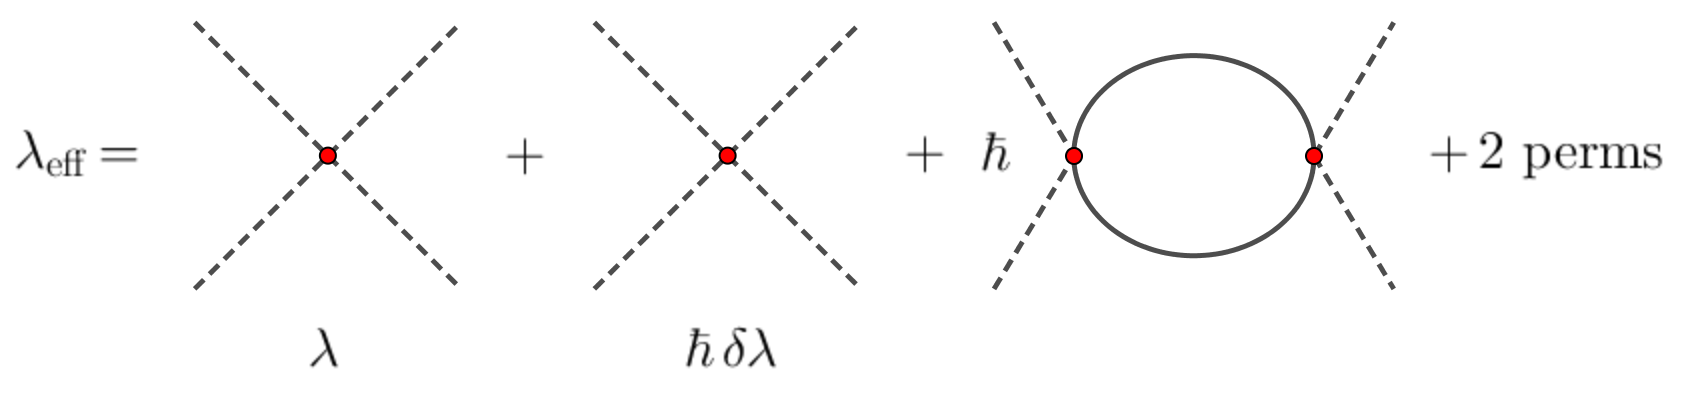
\includegraphics[width=0.9\textwidth]{graphics/aqft/quart1.png}\label{fig:quart1}\end{center}
The loop diagrams in momentum space then have a contribution given by, for example;
\begin{center}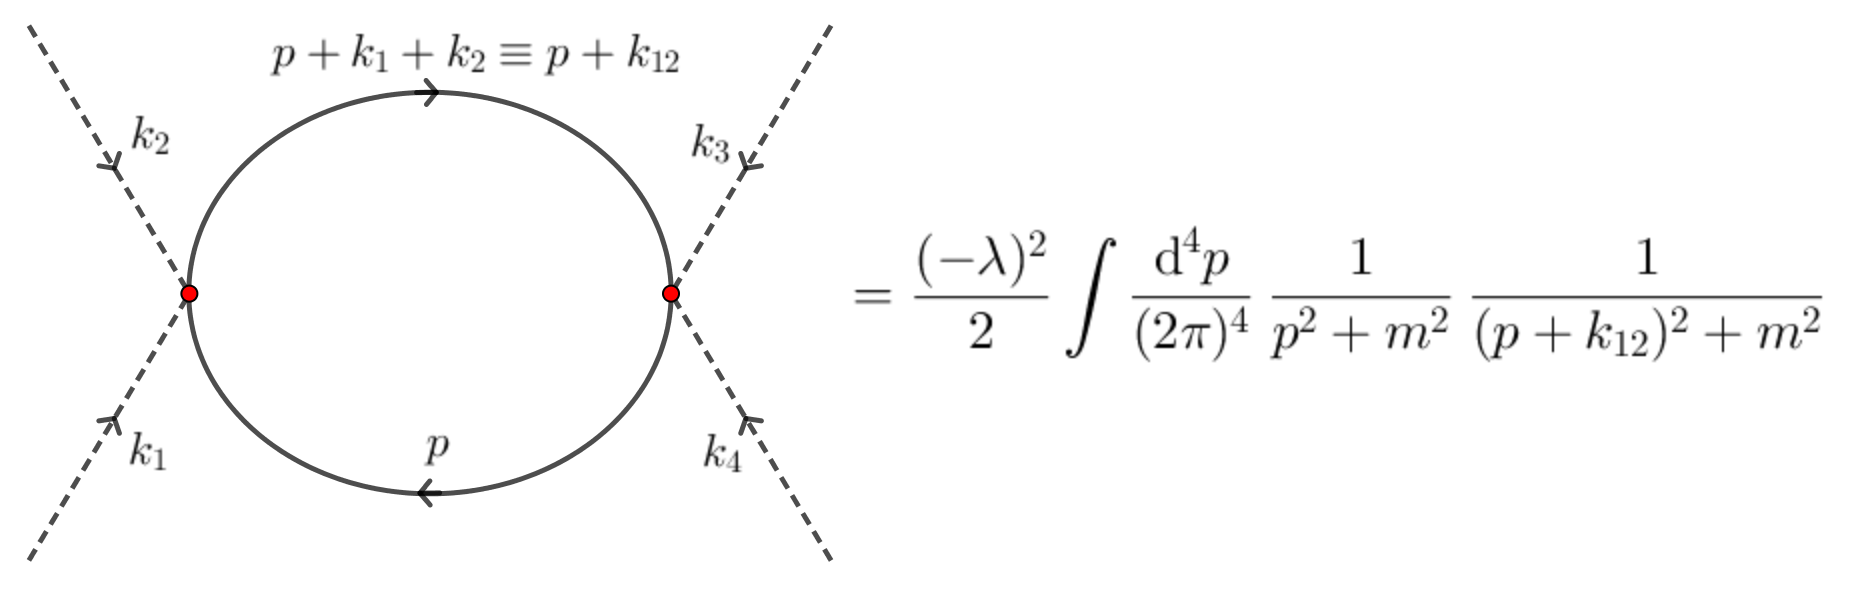
\includegraphics[width=0.7\textwidth]{graphics/aqft/quart2.png}\label{fig:quart2}\end{center}
The fact that these loop integrals depend on the $k_i$ mean that they generate an infinite series of derivative interactions in $\Gamma$ such as $\del_\mu \phi \del^{\mu} \phi \phi^2$. The contribution to the pure $\phi^4$ vertex is independent of the $k_i$ so it is given by;
\begin{equation*}
3 \frac{\lambda^2}{2} \int^{\Lambda_0}{\frac{\ud^4 p}{(2\pi)^4}\frac{1}{(p^2 + m^2)^2}}
\end{equation*}
since each of the three channels contributes equally. This loop integral is logarithmically divergent as $\Lambda_0 \rightarrow \infty$;
\begin{align*}
\frac{3\lambda^2}{2} \int^{\Lambda_0}{\frac{\ud^4 p}{(2\pi)^4}\frac{1}{(p^2 + m^2)^2}} &= \frac{3 \lambda^2}{32 \pi^4}\text{vol}(\mS^{3})\int_0^{\Lambda_0}{\frac{p^3 \ud p}{(p^2 + m^2)^2}} \\
&= \frac{3\lambda^2}{32\pi^4}\text{vol}(\mS^3)\int_0^{\Lambda_0^2 / m^2}{\frac{u \ud u}{(1 + u)^2}} \\
&= \frac{3\lambda^2}{32\pi^2}\left(\log\left(1 + \frac{\Lambda_0^2}{m^2}\right) - \frac{\Lambda_0^2}{\Lambda_0^2 + m^2}\right)
\end{align*}
To get a finite result for $\lambda_{\text{eff.}}$ we tune our initial $\lambda$ using $\delta \lambda$. We might choose;
\begin{equation}
\delta \lambda = \frac{3\lambda^2}{32\pi^2}\left(\log\left(\frac{\Lambda_0^2}{m^2}\right) - 1\right)
\end{equation}
in which case we find that;
\begin{equation}
\lambda_{\text{eff.}} = \lambda - \frac{3\hbar \lambda^2}{32 \pi^2}\left(\log\left(1 + \frac{m^2}{\Lambda_0^2}\right) + \frac{m^2}{m^2 + \Lambda_0^2}\right) + \mO(\hbar^2)
\end{equation}
\subsubsection{The Role of Irrelevant Couplings}
We neglected derivative terms in $\Gamma$ during this calculations. In general though, these are generated and contribute to four particle scattering processes. Using $\Gamma$ we should use all terms with exactly $4$ $\phi$'s. To calculate these we need to actually evaluate the loop integrals at non-zero external momenta. We make use of Feynman's trick;
\begin{equation*}
\frac{1}{AB} = \frac{1}{B - A}\left.\left(\frac{1}{xA + (1 - x)B}\right)\right|_{0}^{1} = \int_0^{1}{\frac{\ud x}{\left(Ax + (1 - x)B\right)^2}}
\end{equation*}
to rewrite;
\begin{align*}
&\frac{1}{(p^2 + m^2)}\frac{1}{\left((p + k_{12})^2 + m^2\right)} \\
& \quad = \int_0^{1}{\frac{\ud x}{\left(x\left((p + k_{12})^2 + m^2\right) + (1 - x)(p^2 + m^2)\right)^2}} \\
& \quad = \int_{0}^{1}{\frac{\ud x}{(p^2 + m^2 + 2x k_{12}\cdot p + xk_{12}^2)^2}} \\
& \quad = \int_{0}^{1}{\frac{\ud x}{\left[(p - xk_{12})^2 + m^2 + x(1 - x)k_{12}\right]^2}}
\end{align*}
So that if $l = p - xk_{12}$ the loop integral becomes;
\begin{equation*}
\frac{\lambda^2}{2}\int_0^{1}{\upd{x}\int{\frac{\ud^4 l}{(2\pi)^4}\frac{1}{\left(l^2 + m^2 + x(1 - x)k_{12}\right)^2}}}
\end{equation*}
We're supposed to integrate this over $\abs{p} \leq \Lambda_0$, however as $\Lambda_0 \rightarrow \infty$ this only differs from the region $\abs{l} \leq \Lambda_0$ by terms of order $k_{12} / \Lambda_0$ which become negligible. In this regime, the loop integral is;
\begin{align*}
&\frac{\lambda^2}{32\pi^4}\text{vol}(\mS^3)\int_0^{1}{\upd{x}\int{\frac{l^3 \ud l}{\left(l^2 + m^2 + x(1 - x)k_{12}^2\right)^2}}} \\
&\quad = \frac{\lambda^2}{32\pi^2}\int_0^{1}{\upd{x}\left(\log\left(\frac{\Lambda_0^2}{m^2 + x(1 - x)k_{12}^{2}}\right) - 1\right)} + \underbrace{\mO\left(\frac{m}{\Lambda_0}, \frac{\abs{k_{12}}}{\Lambda_0}\right)}_{\text{vanishes as }\Lambda_0 \rightarrow \infty}
\end{align*}
Then the total contribution to the $4$-scalar amplitude is;
\begin{align*}
&\mathcal{A}(k_i) = \lambda + \hbar \delta \lambda - \frac{\lambda^2 \hbar}{32 \pi^2}\int_0^{1}{\upd{x}}\left[ \log \frac{\Lambda_0^2}{m^2 + x(1 - x)k_{12}^2} \right.\\
&\qquad \left. + \log \frac{\Lambda_0^2}{m^2 + x(1 - x)k_{23}^2} + \log \frac{\Lambda_0^2}{m^2 + x(1 - x)k_{13}^2} - 3\right]  \\
& \qquad + \mO(\hbar^2, m/\Lambda_0, \abs{k_i}/\Lambda_0)
\end{align*}
Using our earlier choice for $\delta \lambda$ this becomes;
\begin{align*}
&\mathcal{A}(k_i) = \lambda - \frac{\lambda^2 \hbar}{32\pi^2} \int_0^{1}{\upd{x}}\left[ \log\frac{m^2}{m^2 + x(1 - x)k_{12}^2} + \log\frac{m^2}{m^2 + x(1 - x)k_{23}^2}\right. \\
& \qquad \left. + \log\frac{m^2}{m^2 + x(1 - x)k_{13}^2}\right] + \mO(\hbar^2)
\end{align*}
At this order in $\hbar$, we have $\lambda = \lambda_{\text{eff}}$ so that whilst we have generated infinitely many derivative interactions in $\Gamma$, however, they are all finite and completely determined by the values of $(m_p, \lambda_{\text{eff}})$. Now consider starting from a more general classical action at a scale $\Lambda_0$;
\begin{equation*}
S_{\Lambda_0}[\phi] = \int{\upd{^4 x}\frac{1}{2}(\del \phi)^2 + \frac{m^2}{2}\phi^2 + V(\phi)}, \quad V(\phi) = \sum_{k \geq 2}{g_{2k}\Lambda_0^{4 - 2k}\phi^{2k}}
\end{equation*}
At one-loop we now get new contributions to the coefficient of $\phi^{2m}$ in $\Gamma$ coming from the $1$PI e.g. those in \autoref{fig:quart3}. 
\begin{mygraphic}{aqft/quart3}{0.8}{The $1$PI diagrams contributing to the coefficient of $\phi^{2m}$. Each graph has $2m$ external legs in total.}{quart3}\end{mygraphic}
Note that the coefficient of $\phi^{2m}$ is just that coming from the expansion of;
\begin{equation*}
\frac{1}{2}\log \det \left(-\del^2 + m^2 + V^{\prime\prime}(\phi)\right)
\end{equation*}
Now, a loop graph with $e$ propagators contributes an amount proportional to;
\begin{equation*}
\int^{\Lambda_0}{\upd{^4 p }\prod_{j = 1}^{e}{\frac{1}{(p + k_j)^2 + m^2}}}
\end{equation*}
for some $k_j$. As $\Lambda_0 \rightarrow \infty$, this is UV finite unless $e = 1$ ($\Lambda_0^2$ divergent) or $e = 2$ ($\log \Lambda_0$ divergent). Also every time we include a $g_{2k + 2}$ vertex we introduce a power $\Lambda_0^{2 - 2k}$ which a suppression if $k > 1$. In other words, for six or more particles at the vertex. Hence we only get contributions in the continuum limit to $\Gamma$ from graphs built solely from a $\phi^4$ vertex together with a finite correction from the graph with $4$ external legs meeting at a point of a loop $\propto g_6$. We can this latter contribution in our renormalisation scheme.
\subsection{Dimensional Regularisation}\index{dimensional regularisation}
This is qualitatively different to the previous methods of regularisation. It is not a way of regularising the path integral measure, instead we are looking for a way to regularise the asymptotic series that results from the loop integrals. First, make the observation that for any given coupling, it's status as marginal, relevant etc. is dependent on the dimension $d = \dim \mM$. As an example, consider the mass correction at one loop in $\phi^4$ theory. Again we only consider the first diagram in \autoref{fig:phi4two} which contributes;
\begin{equation*}
-\frac{\lambda}{2(2\pi)^4}\int{\frac{\ud^4 p}{p^2 + m^2}} \overset{d \in \mathbb{N}}{\longrightarrow} - \frac{1}{2}\frac{g(\mu) \mu^{4 - d}}{(2\pi)^d} \int{\frac{\ud^d p}{p^2 + m^2}}
\end{equation*}
where we have introduced the dimensionless coupling $g(\mu) = \lambda \mu^{d - 4}$. Now $\mu$ is just some arbitrary scale (e.g. the energy scale of our experiment). Importantly it is \emph{not} a cut off, and so does not take values up to infinity. Then;
\begin{equation*}
-\frac{1}{2}\frac{g(\mu)\mu^{4 - d}}{(2\pi)^{d}}\int{\frac{\ud^d p}{p^2 + m^2}} = -\frac{g(\mu) \mu^{4 - d}}{2(2\pi)^{d}}\text{vol}(\mS^{d - 1})\int_0^{\infty}{\upd{p}\frac{p^{d - 1}}{p^2 + m^2}}
\end{equation*}
To compute the volume (read volume of the manifold not of the $d$-ball), we note that;
\begin{equation*}
\pi^{d/2} = \int_{\RR^{d}}{\prod_{i = 1}^{d}{e^{-x_i^2}}\,\,\ud x_i} = \text{vol}(\mS^{d - 1})\int_0^{\infty}{\upd{r}r^{d - 1}e^{-r^2}} = \text{vol}(\mS^{d - 1})\frac{1}{2}\Gamma\left(\frac{d}{2}\right)
\end{equation*}
So we find that whenever $d \in \mathbb{N}$;
\begin{equation}
\text{vol}(\mS^{d - 1}) = \frac{2\pi^{d/2}}{\Gamma\left(\frac{d}{2}\right)}
\end{equation}
We now define this expression to be $\text{vol}(\mS^{d - 1})$ for $d \in \CC$. The rest of the integral is then;
\begin{align*}
\mu^{4 - d}\int_0^{\infty}{\frac{p^{d - 1}\ud p}{p^2 + m^2}} &= \frac{1}{2}\mu^{d - 4}\int_0^{\infty}{\frac{(p^2)^{(d/2) - 1}\ud (p^2)}{p^2 + m^2}} \\
&= \frac{m^2}{2}\left(\frac{\mu}{m}\right)^{4 - d} \underbrace{\int_0^{1}{(1 - u)^{(d/2) - 1}u^{-d/2}\ud u}}_{\text{beta function}} \\
&= \frac{m^2}{2}\left(\frac{\mu}{m}\right)^{4 - d} \frac{\Gamma(d/2) \Gamma(1 - d/2)}{\Gamma(1)}
\end{align*}
Thus we find that in dimensional regularisation the one loop contribution to $\Pi(k^2)$ is;
\begin{equation*}
\Pi(k^2) = - \frac{g(\mu)m^2}{2(4\pi)^{d/2}}\left(\frac{\mu}{m}\right)^{4 - d} \Gamma(1 - d/2)
\end{equation*}
We should analytically continue this to $d = 4$ by setting $d = 4 - \epsilon$ and using the result;
\begin{equation*}
\Gamma(\epsilon) \sim \frac{1}{\epsilon} - \gamma + \mO(\epsilon)
\end{equation*}
where $\gamma$ is the Euler-Mascheroni constant\index{constant!Euler-Mascheroni}, then we have;
\begin{equation*}
\Pi_{\text{\footnotesize{1-loop}}}(k^2) \sim \frac{g(\mu)m^2}{32\pi^2} \left(\frac{2}{\epsilon} - \gamma + \log\left(\frac{4\pi\mu^2}{m^2}\right)\right) + \mO(\epsilon)
\end{equation*}
The divergence in the $1$-loop $\Pi(k^2)$ as $\Lambda_0 \rightarrow \infty$ has become the pole $1/\epsilon$. In particular note that the logarithm is perfectly finite since $\mu$ is not a cut off.
\subsubsection{The $\bar{\text{\textbf{MS}}}$ Renormalisation Scheme}
We fix the counterterm $\delta m^2$ by requiring a finite result in $d = 4$ so we have to remove the $1/\epsilon$ term. Just doing this is minimal substitution (MS). Often it is convenient to also remove the $\gamma$ and $4\pi$ terms. This is modified minimal subtraction. So we choose;
\begin{equation*}
\delta m^2 = - \frac{g(\mu)m^2}{32\pi^2}\left(\frac{2}{\epsilon} - \gamma + \log 4\pi\right)
\end{equation*}
in the $\bar{\text{MS}}$ scheme. Thus we have;
\begin{equation*}
\Pi(k^2) = \frac{g(\mu)m^2}{32\pi^2}\log\left(\frac{\mu^2}{m^2}\right)
\end{equation*}
which is now finite as $d \rightarrow 4$. For the $\phi^4$ term, the loop corrections come from the same integrals computed above in the renormalisation of the quartic coupling;
\begin{equation*}
\frac{g^{2}(\mu)\mu^{4 - d}}{2}\int{\frac{\ud^{d}p}{(2\pi)^{d}}\frac{1}{p^2 + m^2}\frac{1}{(p + k_{12})^2 + m^2}}
\end{equation*}
along with other channels. Again if we are just interested in the pure quartic coupling then we can set $k_{ij} = 0$ and find the contribution;
\begin{align*}
\frac{3g^{2}(\mu)\mu^{4 - d}}{32\pi^4}\text{vol}(\mS^{d - 1})\int_0^{\infty}{\frac{p^{d - 1}\ud p}{(p^2 + m^2)^2}} &= \frac{3g^2}{2(4 \pi)^{d/2}}\left(\frac{\mu}{m}\right)^{4 - d}\Gamma(2 - d/2) \\
&\sim \frac{3g^2}{32\pi^2}\left(\frac{2}{\epsilon} - \gamma + \log\frac{4\pi \mu^2}{m^2}\right) + \mO(\epsilon) 
\end{align*}
Then we choose out counterterm to remove this pole;
\begin{equation}
\delta g = \frac{3g^2}{32\pi^2}\left(\frac{2}{\epsilon} - \gamma + \log 4\pi\right)
\end{equation}
again in the $\bar{\text{MS}}$ scheme. So we find a $\phi^{4}$ coupling in the $1$PI effective action of;
\begin{equation*}
g_{\text{eff}}(\mu) = g(\mu) - \frac{3\hbar g^{2}(\mu)}{32\pi^2}\log\left(\frac{\mu^2}{m^2}\right) + \mO(\hbar^2)
\end{equation*}
The scale $\mu$ was merely a choice of units and we are now in exactly $d = 4$ so $g_{\text{eff}}$ can't depend on $\mu$. This is compatible with our result if;
\begin{align*}
\mu\frac{\del g_{\text{eff}}}{\del \mu} &= 0 = \mu\frac{\del}{\del \mu}\left(g(\mu) - \frac{3\hbar g^2(\mu)}{16\pi^2}\log\left(\frac{\mu}{m}\right) + \mO(\hbar^2)\right) \\
\Rightarrow \beta(g) &= \mu \frac{\del g}{\del \mu} = \frac{3\hbar g^2}{16\pi^2} + \mO(\hbar^2)
\end{align*}
i.e. $g(\mu)$ is marginally irrelevant. Solving this for the coupling we see that;
\begin{equation}
\frac{1}{g(\mu\pr)} = \frac{1}{g(\mu)} + \frac{3\hbar}{16\pi^2}\log\left(\frac{\mu}{\mu\pr}\right) + \mO(\hbar^2)
\end{equation}
Now, if we just solved the original path integral exactly, we would find of course that $\Gamma(\phi)$ is independent of $\mu$. But since we are working perturbatively, it is ambiguous as to whether we should do perturbation theory in $g(\mu)$ or $g(\mu\pr)$. In fact we actually have no choice; there is a scale inherent in $\phi^4$ theory, $\mu\pr = \Lambda_{\phi^4}$ where $g(\mu\pr)^{-1} = 0$. In other words we find;
\begin{equation*}
g(\mu) = \frac{16\pi^2}{3\hbar}\frac{1}{\log(\Lambda_{\phi^4}/\mu)}
\end{equation*}
\subsection{One-loop Renormalisation of QED}\index{QED}
We start with the action;
\begin{equation}
S_{\text{QED}} = \int{\upd{^4 x}\frac{1}{4e^2}F_{\mu\nu}F^{\mu\nu} + \bar{\psi}(\slashed{D} + m)\psi}
\end{equation}
where $D_\mu = \del_\mu + i A_\mu$ and $(\gamma^{\mu})\dagg = - \gamma^{\mu}$ in the Euclidean signature. THis means that the $\text{SO}(4)$ generators $S^{\mu\nu} = \tfrac{1}{4}[\gamma^{\mu}, \gamma^{\nu}]$ are all hermitian and $\bar{\psi} = \psi\dagg$. We rescale the photon field; $A^{\text{new}} = A^{\text{old}}/e$ so that;
\begin{equation*}
S_{\text{QED}}[A^{\text{new}}, \psi] = \int{\upd{^4 x}\frac{1}{4}F^2 + \bar{\psi}(\slashed{\del} + m)\psi + ie\bar{\psi}\slashed{A}\psi}
\end{equation*}
In momentum space, the Maxwell term becomes;
\begin{equation*}
\frac{1}{4}\int{\upd{^4 x}F_{\mu\nu}F^{\mu\nu}} = \frac{1}{2}\int{\upd{^4 k}k^2 \left(\delta^{\mu\nu} - \frac{k^{\mu}k^{\nu}}{k^2}\right)A_{\mu}(-k)A_{\nu}(k)}
\end{equation*}
from which we can read off the free photon propagator;
\begin{equation*}
\Delta^{(0)}_{\mu\nu}(k) = \frac{1}{k^2}\left(\delta^{\mu\nu} - \frac{k^{\mu}k^{\nu}}{k^2}\right)
\end{equation*}
In the Lorenz gauge\index{gauge!Lorenz}, $\del^{\mu}A_\mu = 0$ which gives the gauge condition $k^{\mu}\Delta^{(0)}_{\mu\nu}(k) = 0$. This implies that only transverse polarisations propagate.
\subsubsection{Vacuum Polarisation}\index{polarisation!vacuum}
In the quantum theory, the exact photon propagator receives corrections as the photon interacts with the electron;
\begin{align*}
\Delta_{\mu\nu}(k) &= \int{\upd{^4 x}e^{ik\cdot x}\left< A_{\mu}(x)A_{\nu}(0) \right>} \\
&= \Delta_{\mu\nu}^{(0)}(k) + \Delta^{(0)}_{\mu \rho}(k)\Pi^{\rho\sigma}(k)\Delta^{(0)}_{\sigma \nu}(k) + \cdots
\end{align*}
where $\Pi_{\rho \sigma}(k)$ is the sum of all $1$PI diagrams with $2$ external photons. This takes the form;
\begin{equation*}
\Pi_{\rho \sigma} = k^2\left(\delta_{\rho \sigma} - \frac{k_\rho k_\sigma}{k^2}\right)\pi(k^2)
\end{equation*}
for some function $\pi(k^2)$. Then the factor in brackets is a projection operator $P\indices{^{\rho}_{\sigma}}$ satisfying $P\indices{^{\rho}_{\kappa}}P\indices{^{\kappa}_{\sigma}} = P\indices{^{\rho}_{\sigma}}$. Then we see that;
\begin{equation*}
\Delta_{\mu\nu}(k) = \Delta_{\mu\nu}^{(0)}(k)\left(1 + \pi(k^2) + \pi^2(k^2) + \cdots\right). = \frac{\Delta_{\mu\nu}^{(0)}(k)}{1 - \pi(k^2)}
\end{equation*}
Just as in the scalar case where the classical propagator was the inverse of the kinetic term in the effective action, here we have;
\begin{equation*}
\Gamma_{\text{eff}}[A] = \frac{1}{2}\int{\upd{^4 k} \left(1 - \pi(k^2)\right)A_\mu(-k)k^2 \left(\delta^{\mu\nu} - \frac{k^{\mu}k^{\nu}}{k^2}\right)A_\nu(k)}
\end{equation*}
In particular expanding $\pi(k^2) = \pi(0) + \cdots$ the leading piece gives;
\begin{equation*}
\Gamma_{\text{eff}}^{(2)}[A] = \int{\upd{^4 x}\frac{1 - \pi(0)}{4}F_{\mu\nu}F^{\mu\nu}}
\end{equation*}
Which governs the leading order wavefunction renormalisation.\index{renormalisation!wavefunction} We compute this via dimensional regularisation, and introduce a dimensionless coupling $g^2(\mu) = e^2 \mu^{d - 4}$ for some experimental scale $\mu$. The vertex is then;
\begin{equation*}
ig(\mu)\mu^{(4 - d)/2}\int{\upd{^d x}\bar{\psi}\slashed{A}\psi}
\end{equation*} 
The leading order correction is then governed by the diagram;
\begin{mygraphic}{aqft/vacpol}{0.8}{The leading order correction to the photon propagator.}{vacpol}\end{mygraphic}
Before writing down the correction, we should understand that a loop in a fermion diagram introduces an overall minus sign. This is really a statement of Wick's theorem and the fact that the components of $\psi$ are Grassman variables. Expanding $\exp\left(- S_{\text{QED}}[A, \psi]/\hbar\right)$ in powers of the vertex we have contributions of the form;
\begin{equation*}
\left< \bar{\psi} \gamma^{\mu}\psi(x_1) \bar{\psi} \cdots \psi(x) \bar{\psi}\gamma^{\rho}\psi(x_n) \right>
\end{equation*}
Joining up $\psi \bar{\psi}$ contributions we find that the first and last are in the opposite order. To get a propagator we need to bring the $\psi$ past the $\bar{\psi}$ which introduces an extra minus sign. Then we find;
\begin{align*}
\Pi^{\rho \sigma}_{\text{1-loop}}(k) &= -(-ig)^2 \mu^{4 - d}\int{\frac{\ud^d p}{(2\pi)^d}\tr\left(\frac{1}{i\slashed{p} + m}\gamma^{\rho}\frac{1}{i(\slashed{p} - \slashed{k}) + m}\gamma^{\sigma}\right)} \\
&= \frac{g^2(\mu)\mu^{4 - d}}{(2\pi)^d}\int{\upd{^d p}\frac{\tr \left((-i \slashed{p} + m)\gamma^{\rho}(-i \slashed{p} - i\slashed{k} + m)\gamma^{\sigma}\right)}{(p^2 + m^2)\left((p - k)^2 + m^2\right)}}
\end{align*}
This integral can be done (apparently) and we find;
\begin{equation}
\Pi_{\text{1-loop}}^{\rho\sigma}(k^2) = (k^2 \delta^{\rho\sigma} - k^{\rho}k^{\sigma})\pi_{\text{1-loop}}(k^2)
\end{equation}
where;
\begin{equation}
\pi_{\text{1-loop}}(k^2) = \frac{-8 g^{2}(\mu)\Gamma(2 - d/2)}{(4\pi)^{d/2}}\int_0^{1}{\upd{x} x(1 - x)\left(\frac{\mu^2}{\Delta}\right)^{2 - d/2}}
\end{equation}
where $\Delta = m^2 + k^2 x(1 - x)$. This expression diverges in $d = 4$ as we would expect, so we need to tune using a couterterm;
\begin{equation*}
\int{\frac{\delta Z_3}{4}F_{\mu\nu}F^{\mu\nu}}
\end{equation*}
Writing $d = 4 - \epsilon$ we have;
\begin{equation*}
\pi_{\text{1-loop}}(k^2) \sim -\frac{g^2(\mu)}{2\pi^2}\int_0^{1}{\upd{x}x(1 - x)\left(\frac{2}{\epsilon} - \gamma + \log \frac{4\pi \mu^2}{\Delta} + \mO(\epsilon)\right)}
\end{equation*}
In the $\bar{\text{MS}}$ scheme then, we take $\delta Z_3$ to absorb the divergent parts of the above;
\begin{equation}
\delta Z_3 = -\frac{g^2(\mu)}{12\pi^2}\left(\frac{2}{\epsilon} - \gamma + \log 4\pi\right)
\end{equation}
So we find that $\Pi^{\rho\sigma}(k^2) = k^2 P^{\rho\sigma}\pi(k^2)$ with;
\begin{equation}
\pi(k^2) = \frac{g^2}{2\pi^2}\int{\upd{x}x(1 - x)\log\left(\frac{m^2 + x(1 - x)k^2}{\mu^2}\right)} + \mO(\hbar, \epsilon)
\end{equation}
\subsubsection{The $\beta$-function of QED}
We have;
\begin{align*}
\Gamma_{\text{eff}}[A^{\text{old}}] &= \frac{1}{4g_{\text{eff}}^2}\int{\upd{^4 x}F_{\mu\nu}F^{\mu\nu}} + \cdots \\
&= \frac{1 - \pi(0)}{4g^2(\mu)}\int{\upd{^4 x} F^2 + \cdots} \\
&= \frac{1}{4}\left(\frac{1}{g^2(\mu)} - \frac{\hbar}{12\pi^2}\log\left(\frac{m^2}{\mu^2}\right) + \mO(\hbar^2)\right)\int{\upd{^4 x}F^2}
\end{align*}
So our vacuum polarisation result also tells us the $\beta$-function of QED. Since the physically measured coupling $g_{\text{eff}}(\mu)$ cannot depend on $\mu$ we have;
\begin{equation*}
0 = \mu\frac{\del}{\del \mu}\left(\frac{1}{g^2} - \frac{\hbar}{12\pi^2} \log\frac{m^2}{\mu^2} + \mO(\hbar^2)\right)
\end{equation*}
So we find that;
\begin{align*}
-\frac{2}{g^3(\mu)}\beta(g) + \frac{\hbar}{6\pi^2} + \mO(\hbar^2) &= 0 \Rightarrow \beta(g) = \frac{\hbar g^3}{12\pi^2} + \mO(\hbar^2)
\end{align*}
Thus we find that;
\begin{equation}
\frac{1}{g^{\prime 2}(\mu\pr)} = \frac{1}{g^2(\mu)} + \frac{\hbar}{6\pi^2}\log\left(\frac{\mu}{\mu\pr}\right)
\end{equation}
From experiment we know that at $\mu \sim m_e \sim 511 \,\,\text{keV}$, we have $\alpha \sim 1/137$, which gives;
\begin{equation*}
g^2(\mu) = \frac{6\pi^2}{\hbar} (\log\frac{\Lambda_{\text{QED}}}{\mu})^{-1}
\end{equation*}
where $\Lambda_{\text{QED}} \sim 10^{236}\,\,\text{GeV}$. So again as in the case of $\phi^4$, there is no continuum theory of QED, it is only valid up to the scale determined by $\Lambda_{\text{QED}}$. This is of no practical consequence as QED ultimately merges with the weak force at an energy scale far below $\Lambda_{\text{QED}}$.
\newpage
\section{Symmetries in QFT}
Suppose we have a change of variables $\phi^a \mapsto \phi^{\prime a} = \phi^a + \epsilon^{r}f^{a}_r(\phi, \del_\mu \phi)$, such that the Lagrangian transforms as $\mL \mapsto \mL + \del^\mu(K_{\mu r} \epsilon^r)$, then the equations of motion will be unaffected and we say that the transformation is symmetry of the classical theory. Noether's theorem further tells us that the current;
\begin{equation*}
J_{\mu r} = \frac{\delta \mL}{\delta(\del^\mu \phi^a)}f_r^a(\phi, \del_\mu \phi) - K_{\mu r}
\end{equation*}
is conserved if the equations of motion hold. We need to re-examine this in the quantum theory. We have two options;
\begin{itemize}
\item Look at general correlation functions
\item Look at the quantum effective action\index{action!quantum effective}
\end{itemize}
We will begin with the second point of view.
\subsection{Symmetries of the Effective Action}
Formally, under $\phi^a \mapsto \phi^{\prime a}$ we would expect $\mD \phi \mapsto \mD \phi\pr$ where;
\begin{equation*}
\mD \phi\pr = \mD \phi \det\left(\frac{\delta \phi^{\prime a}(x)}{\delta \phi^b(y)}\right)
\end{equation*} 
where;
\begin{equation*}
\frac{\delta \phi^{\prime a}(x)}{\delta \phi^b(y)} = \delta\indices{^{a}_{b}}\delta(x - y) + \epsilon^{r}\frac{\delta f_r^a(\phi, \del \phi)}{\delta \phi^b(y)} + \mO(\epsilon^2)
\end{equation*}
So we find that;
\begin{equation*}
\det\left(\frac{\delta \phi^{\prime a}(x)}{\delta \phi^b(y)}\right) = 1 + \tr \epsilon^r \frac{\delta f_r^a(\phi, \del \phi)}{\delta \phi^b(y)} + \mO(\epsilon^2)
\end{equation*}
which is a trace over the flavour indices $a, b$ as well as a functional trace over $x, y$. We'll be interested in transformations for which $\mD \phi = \mD \phi\pr$. In this case consider the partition function;
\begin{equation*}
\mZ[\vec{J}] = \int{\mD \phi\pr \,\,\exp\left(-\frac{1}{\hbar}\left(S[\phi] + \int{\upd{^d x}J_a(x)\phi^{\prime a}(x)}\right)\right)}
\end{equation*}
Using the fact that we have a symmetry;
\begin{align*}
\mZ[\vec{J}] &= \int{\mD \phi \,\,\exp\left(-\frac{1}{\hbar}\left(S[\phi] + \int{\upd{^d x}J_a(x)\phi^a(x)} + \int{\upd{^d x}J_a \epsilon^r f^a_r}\right)\right)} \\
&= \int{\mD \phi \,\, \exp\left(- \frac{1}{\hbar}\left(S[\phi] + \int{\upd{^d x}J\phi}\right)\right)} \\ 
&\qquad \qquad \qquad \qquad \times \left\{1 - \frac{\epsilon^r}{\hbar}\int{\upd{^d x}J_a f_r^a(\phi, \del \phi)} + \mO(\epsilon^2)\right\} \\
&= \mZ[\vec{J}] - \frac{\epsilon^r}{\hbar}\mZ[\vec{J}] \left< \int{\upd{^d x}J_a f^a_r(\phi, \del\phi)} \right>_{\vec{J}} + \mO(\epsilon^2)
\end{align*}
So we see that this implies;
\begin{equation}
\int{\upd{^d x}J_a(x)\left< f^a_r(\phi, \del \phi) \right>_{\vec{J}}} = 0
\end{equation}
We want to write this in terms of the quantum effective action, $\Gamma[\Phi]$. Recall that $\Gamma[\Phi]$ is the Legendre transform of $W[\vec{J}]$ where $\vec{J}$ is evaluated at the extremum;
\begin{equation*}
J_\phi^a = -\frac{\delta \Gamma[\Phi]}{\delta \Phi^a}
\end{equation*}
such that $\left< \phi^a \right>_{\vec{J}_\phi} = \Phi^a$, where $\Phi^a$ is the field in the $1$PI effective action. At this value, our condition becomes;
\begin{equation*}
\int{\upd{^d x}\frac{\delta \Gamma[\Phi]}{\delta \Phi^a} \left< f_r^a(\phi, \del \phi) \right>_{\vec{J}_\phi}} = 0
\end{equation*}
In other words, the quantum effective action is invariant under;
\begin{equation*}
\Phi^a \mapsto \Phi^{\prime a} = \Phi^a + \epsilon^r \left< f^a_r(\phi, \del \phi) \right>_{\vec{J}_\phi}
\end{equation*}
As a special case (and an important one), suppose that $f$ is actually linear in $\phi$ i.e.
\begin{equation*}
f^a_r(\phi, \del\phi) = c_r^a(x) + \int{\upd{^d x}d_{rb}(x, y)\phi^b(y)}
\end{equation*}
Then we have the following (note that this \emph{only} holds in the case that $f$ is linear);
\begin{equation}
\left< f^a_r(\phi, \del \phi) \right>_{\vec{J}_\phi} = f_r^a\left(\left< \phi \right>_{\vec{J}_\phi}, \left< \del \phi \right>_{\vec{J}_\phi}\right) = f_r^a(\Phi, \del \Phi)
\end{equation}
Thus, in this case, $\Gamma[\Phi]$ is invariant under $\Phi^a \mapsto \Phi^a + \epsilon^r f_r^a(\Phi, \del \Phi)$, and so has th same symmetry as the classical action, $S[\phi]$. So if we can find a classical action with a symmetry at linear order under which the path integral measure is invariant, then it will be a symmetry of the full quantum theory. As an example consider;
\begin{equation*}
S[\phi] = \int{\upd{^d x}\frac{1}{2}(\del\phi)^2 + \frac{1}{2}m^2 \phi^2 + \lambda \phi^4}
\end{equation*}
then $S[\phi] = S[-\phi]$. Now, \emph{provided we regularise} in a way that is compatible with this $\ZZ_2$ symmetry, we will also have $\Gamma[\Phi] = \Gamma[-\Phi]$ i.e. we can't generate terms like $\Phi^3, \Phi^7$ etc. As another example suppose we have the action;
\begin{equation*}
S[\phi^a] = \int{\upd{^d x}\frac{1}{2}\delta_{ab}\del \phi^a \del \phi^b + \frac{m^2}{2}\delta_{ab}\phi^a \phi^b + \frac{\lambda}{4}(\phi^a \phi^b \delta_{ab})^2}
\end{equation*}
then this is invariant under $\text{SO}(n)$ rotations $\phi^a \rightarrow \phi^a + \omega\indices{^{a}_{b}}\phi^b$ so that;
\begin{equation*}
\frac{\delta f^a(\phi, \del \phi)}{\delta \phi^b(y)} = \omega\indices{^{a}_{b}}\delta(x - y)
\end{equation*}
which is field independent. So provided we treat all components of the field the same when we regularise, the effective action will also be $\text{SO}(n)$ invariant.

\paraskip
As a final example, suppose we have an $\text{SO}(d)$ transformation of the co-ordinate system $x^{\mu}\mapsto L\indices{^{\mu}_{\nu}}x^{\nu}$ with $L \in \text{SO}(d)$. This induces a transformation on the fields;
\begin{equation*}
A_\mu(x) \mapsto (L^{-1})\indices{_{\mu}^{\nu}}A_\nu(L^{-1}x) , \quad \psi^\alpha \mapsto S\indices{^{\alpha}_{\beta}}(L)\psi^\beta(L^{-1}x)
\end{equation*}
where $S\indices{^{\alpha}_{\beta}}(L) = \exp(\tfrac{i}{4}L_{\mu\nu}[\gamma^\mu, \gamma^\nu])\indices{^{\alpha}_{\beta}}$ are the $\text{SO}(d)$ generators in the Dirac spinor representation. Then, $S_{\text{QED}}[A, \psi]$ is $\text{SO}(d)$ invariant, and so to will $\Gamma_{\text{QED}}[A, \psi]$ provided we regularise in an $\text{SO}(d)$ invariant way.\footnote{This might be by imposing a cut off on the eigenvalues of $-\Box$, or working with $d \in \CC$, but it will \emph{not} be by working on a lattice $\Lambda \subset \RR^{d}$, which will not respect the full $\text{SO}$(d) invariance.} In general, there are three possibilities;
\begin{enumerate}
\item There exists a symmetry compatible regularisation which we go ahead and use. Then the regularised quantum theory will also have this symmetry manifest at every stage.
\item There exists a symmetry compatible regularisation which we do not use. In this case the regularised theory and counterterms will not respect the symmetry. However, the symmetry will be restored in the continuum limit.
\item There does not exist any symmetry compatible regularisation. The symmetry is then absent in the quantum theory despite being present at the classical level, and is said to be an \emph{anomaly}\index{anomaly}. 
\end{enumerate}
As an explicit example of this last point, consider;
\begin{equation*}
S[\phi] = \int{\upd{^4 x}\frac{1}{2}(\del \phi)^2 + \frac{\lambda}{4!}\phi^4}
\end{equation*}
This is invariant under conformal transformations\index{conformal transformation}, $\delta \mapsto e^{2\sigma}\delta$, $\phi \mapsto e^{-\sigma}\phi$ where $\sigma \in \RR$. Since $\mC = \set{\phi : \RR^4 \rightarrow \RR}$ is a vector space, we could give it a metric;
\begin{equation*}
\ud s^2_{\mC} = \int_{\RR^4}{\upd{^4 x}\abs{\delta \phi}^2}
\end{equation*}
and take the path integral measure to be the Riemannian measure associated to this metric. But this measure is \emph{not} conformally invariant. We thus do not expect our quantum theory to be conformal, and indeed this is confirmed in the beta functions.
\subsection{Ward-Takahashi Identities}\index{Ward-Takahashi identity}
Symmetries also place constraints on the correlation functions. Suppose $\mO_i(\phi)$ vary under a symmetry transformation $\phi \mapsto \phi\pr$ as $\mO_i(\phi) \mapsto \mO_i(\phi\pr)$ (i.e. they have no spin indices etc.), then;
\begin{equation*}
\int{\mD \phi\pr\,\,e^{-S[\phi\pr]/\hbar}\mO_1\left(\phi\pr(x_1)\right)\cdots\mO_n\left(\phi\pr(x_n)\right)} = \int{\mD \phi\,\,e^{-S[\phi]/\hbar}\prod_{i = 1}^{n}{\mO_i\left(\phi\pr(x_i)\right)}}
\end{equation*}
So we see that this implies;
\begin{equation}
\left< \mO_1\left(\phi(x_1)\right)\cdots\mO_n\left(\phi(x_n)\right) \right> = \left< \mO_1\left(\phi\pr(x_1)\right) \cdots \mO_n\left(\phi\pr(x_n)\right)\right>
\end{equation}
This is the (global) Ward-Takahashi identity. As an example consider the action for a complex scalar field;
\begin{equation*}
S[\phi] = \int{\upd{^d x}\frac{1}{2}\del^{\mu} \bar{\phi}\del_\mu\phi + V\left(\abs{\phi}^2\right)}
\end{equation*}
Then this is invariant under $\phi \mapsto e^{i\alpha}\phi$ and $\bar{\phi} \mapsto e^{-i\alpha}\bar{\phi}$, $\alpha \in \RR$. Then suppose we insert operators of the form $\mO_i(x) = \phi^{r_i}(x)\bar{\phi}^{s_i}(x)$. The Ward-Takahashi identity gives;
\begin{equation*}
\left< \prod_{i = 1}^{n}{\mO_i(x_i)} \right> = \exp\left(i\alpha \sum_{i = 1}^{n}(r_i - s_i)\right)\left< \prod_{i = 1}^{n}{\mO_i(x_i)} \right>
\end{equation*}
and so we deduce that the correlator vanishes unless $\sum{r_i} = \sum{s_i}$ since the above holds for all $\alpha \in \RR$. This is known as a \emph{selection rule}\index{selection rule}.

\paraskip
Similarly, consider spacetime translations $x \mapsto x\pr = x - a$ where $a \in \RR^{d}$. Then $\phi\pr(x) = \phi(x - a)$ for a scalar field. If this is a symmetry then inserting operators that only depend on $x$ through their dependence on the fields implies that;
\begin{equation*}
\left< \prod_{i = 1}^{n}{\mO_i(x_i)} \right> = \left< \prod_{i = 1}^{n}{\mO_{i}(x_i - a)} \right>
\end{equation*}
which allows us to deduce that the correlator can only be a function of the differences $\left(x_i - x_j\right)$. Suppose further that our theory was $\text{SO}(d)$ invariant, then the correlators of scalar operators could only depend on the $\text{SO}(d)$ invariant separations $(x_i - x_j)^2$.
\subsection{Current Conservation in QFT}
Suppose that our transformation $\phi^a \mapsto \phi^a + \epsilon^r f_r^a(\phi, \del \phi)$ leaves the Lagrangian, $\mL(\phi)$, invariant not just the action, and also preserves the path integral measure $\mD \phi$. Then we have a local conservation law for constant $\epsilon$. Just as in Noether's theorem, if we allow $\epsilon^r \mapsto \epsilon^r(x)$, the action can only vary by terms $\del_\mu \epsilon^r(x)$. So our partition function becomes;
\begin{equation*}
\mZ = \int{\mD \phi\pr \,\, e^{-S[\phi\pr]/\hbar}} = \int{\mD \phi e^{-S[\phi]/\hbar}\left(1 - \int_{\mM}{\upd{^d x}j^\mu(x)\del_\mu \epsilon^r(x)} + \mO(\epsilon^2)\right)}
\end{equation*}
where now $j^{\mu}(x)$ may contain contributions from the path integral measure as well as just the field transformation. To first order in $\epsilon^r$ we see that this is simply;
\begin{equation*}
\int_{\mM}{\upd{^d x}\left< j^{\mu}_r(x) \right>\del_\mu \epsilon^r(x)} = 0
\end{equation*}
Integrating by parts, this simply says that the expectation of $\left< j^{\mu}_r(x) \right>$ is conserved;\footnote{With the standard set of assumptions that $\mM$ is compact/there are no boundary terms etc.}
\begin{equation}
\del_\mu \left< j^{\mu}_r(x) \right> = 0
\end{equation}
In the presence of operators, this doesn't hold as is, instead the operators themselves change infinitesimally under the transformation $\phi \mapsto \phi\pr$, 
\begin{equation*}
\mO_i \mapsto \mO_i + \epsilon^r (\delta_r \mO_i)
\end{equation*}
Then carrying out a similar procedure to the one above we find;
\begin{multline*}
\int{\mD\phi\pr\,\,e^{-S[\phi\pr]/\hbar}\prod_{i = 1}^{n}{\mO\pr_i(x_i)}} \\ = \int{\mD \phi\,\,e^{-S[\phi]/\hbar}\left(1 - \int_{\mM}{\upd{^d x}j^\mu_r(x)\del_\mu \epsilon^r(x)} + \mO(\epsilon)\right)} \\ \times \left(\prod_{i = 1}^{n}{\mO_i(x_i)} + \sum_{i = 1}^{n}\epsilon^r(x_i)(\delta_r\mO_i)\prod_{j \neq i}{\mO_j(x_j)}\right)
\end{multline*}
After performing a completely analogous integration by parts and equating the first term with the left hand side, we see that;
\begin{align*}
\int_{\mM}{\upd{^d x}\epsilon^r(x)\del_\mu\left< j_r^{\mu}(x)\prod_{i = 1}^{n}{\mO_i(x_i)} \right>} &= -\sum_{i = 1}^{n}{\epsilon^r(x_i)\left< \left(\delta_r \mO_i(x_i)\right)\prod_{j \neq i}{\mO_j(x_j)} \right>} \\
&\hspace{-100pt}= -\sum_{i = 1}^{n}\int{\upd{^d x}\delta^{(d)}(x - x_i)\epsilon^r(x)\left< \delta_r \mO_i(x_i)\prod_{j \neq i}{\mO_j(x_j)} \right>}
\end{align*}
Thus we find the local form of the Ward-Takahashi identity;
\begin{equation}
\del_\mu\left< j^\mu_r(x)\prod_{i = 1}^{n}{\mO_i(x_i)} \right> = -\sum_{i = 1}^{n}{\delta^{(d)}(x - x_i)\left< \delta_r\mO_i(x_i)\prod_{j \neq i}{\mO_j(x_j)} \right>}
\end{equation}
This generalises current conservation in the classical theory and says that the correlator is conserved except at the operator insertion points, integrating over all of $\mM$ we find;
\begin{equation*}
0 = \sum_{i = 1}^{n}{\left< \delta_r(x_i)\prod_{j \neq i}{\mO(x_j)} \right>} = \delta_r\left< \prod_{i = 1}^{n}{\mO_i(x_i)} \right>
\end{equation*}
which reproduces the global identity for $\phi \mapsto \phi + \delta \phi$.
\subsection{Ward-Takahashi Identity in QED}
The QED action;
\begin{equation*}
S[A, \psi] = \int{\upd{^d x}\frac{1}{4e^2}F_{\mu\nu}F^{\mu\nu} + \bar{\psi}(\slashed{D} + m)\psi}
\end{equation*}
is invariant under the global transformation $\psi \mapsto e^{i\alpha}\psi$, $\bar{\psi} \mapsto e^{-i\alpha}\bar{\psi}$, $A_\mu \mapsto A_\mu$ (so this is not a gauge transformation), where $\alpha \in \RR$. As in our earlier discussion, this is a symmetry of the quantum theory providing our regularised path integral measure integrates over as many $\psi$ modes as $\bar{\psi}$ modes. Now, promoting $\alpha \rightarrow \alpha(x)$ we generate a Noether current $j^{\mu} = i \bar{\psi}\gamma^{\mu}\psi$, assuming that the path integral measure stays invariant. For infinitesimal $\alpha$ we have;
\begin{equation*}
\delta \psi = i \alpha \psi, \qquad \delta \bar{\psi} = -i \alpha \bar{\psi}
\end{equation*}
so that the local Ward-Takahashi identity for $\left< \psi(x_1)\bar{\psi}(x_2) \right>$ is;
\begin{multline*}
\del_\mu\left< j^{\mu}(x)\psi(x_1)\bar{\psi}(x_2) \right> \\ = -i\delta^{(4)}(x - x_1)\left< \psi(x_1)\bar{\psi}(x_2) \right> + \delta^{(4)}(x - x_2)\left< \psi(x_1)\bar{\psi}(x_2) \right>
\end{multline*}
In momentum space we see that;
\begin{align*}
&\int{\ud^4 x_1\upd{^4 x_2}e^{ik_1 \cdot x_1}e^{-ik_2\cdot x_2}\left< \psi(x_1)\bar{\psi}(x_2) \right>} \\
&\hspace{50pt}= \int{\ud^4 x_1 \upd{^4 x_2} e^{ik_1\cdot x_1}e^{-ik_2\cdot x_2}\left< \psi(x_1 - x_2)\bar{\psi}(0) \right>} \\
&\hspace{50pt}= (2\pi)^4 \delta^{(4)}(k_1 - k_2)S(k_1)
\end{align*}
where $S(k)$ is the exact electron propagator, so as before we have;
\begin{align*}
S(k) &= \frac{1}{i\slashed{k} + m} + \frac{1}{i\slashed{k} + m}\Sigma(\slashed{k}) \frac{1}{i\slashed{k} + m} + \cdots \\
&= \frac{1}{i\slashed{k} + m - \Sigma(\slashed{k})}
\end{align*}
where $\Sigma(\slashed{k})$ is the electron self-energy. We can also define the exact electromagnetic vertex $\Gamma_\mu(k_1, k_2)$ as follows;
\begin{align*}
&\int{\ud^4 x\ud^4 x_1 \upd{^4 x_2}e^{ip\cdot x}e^{ik_1\cdot x_1}e^{-ik_2\cdot x_2}\left< j_\mu(x)\psi(x_1)\bar{\psi}(x_2) \right>} \\
&\qquad= \int{\ud^4 x\ud^4 x_1 \upd{^4 x_2}e^{ip\cdot(x - x_2)}e^{ik_1\cdot(x_1 - x_2)}e^{-i(p + k_1 - k_2)\cdot x_2}} \\
&\qquad \qquad \times \left< j_\mu(x - x_2) \psi(x_1 - x_2) \bar{\psi}(0)\right> \\
&\qquad = (2\pi)^4 \delta^{(4)}(p + k_1 - k_2)S(k_1) \Gamma_\mu(k_1, k_2)S(k_2)
\end{align*}
To motivate this last line, note that $j^{\mu} = i\bar{\psi}\gamma^{\mu}\bar{\psi}(x)$ so that in the correlator, $\left< j_\mu(x - x_2) \psi(x_1 - x_2) \bar{\psi}(0)\right>$ we have the term;
\begin{mygraphic}{aqft/emvertex}{0.7}{Illustration of the corrections to the exact EM vertex $\Gamma_\mu(k_1, k_2)$ which cannot be seen as corrections to the propagator.}{emvertex}\end{mygraphic}
So we see that to leading order $\Gamma_\mu = \gamma_\mu + \text{quantum corrections}$, at next leading order, we have the $1$PI part of the exact vertex that look like;
\begin{mygraphic}{aqft/emvertex2}{0.5}{$1$PI corrections to the exact vertex.}{emvertex2}\end{mygraphic}
In momentum space then, the Ward-Takahashi identity becomes;
\begin{align*}
(k_1 - k_2)_{\mu}S(k_1)\Gamma^{\mu}(k_1, k_2)S(k_2) &= i S(k_1) - iS(k_2) \\
\Rightarrow (k_1 - k_2)_\mu \Gamma^{\mu}(k_1, k_2) &= iS^{-1}(k_2) - iS^{-1}(k_1)
\end{align*}
We can differentiate this with respect to $k_1$ and set $k_1 = k_2 = k$, so that;
\begin{align*}
\Gamma_\mu(k_1, k_2) &= -i\frac{\del}{\del k^{\mu}}S^{-1}(k) = -i\frac{\del}{\del k^{\mu}}\left(i \slashed{k} + m + \Sigma(\slashed{k})\right) \\
\Rightarrow \Gamma_{\mu}(k, k) &= \gamma^{\mu} - i\frac{\del}{\del k^{\mu}}\Sigma(\slashed{k})
\end{align*}
This is important in the sense that it shows that the \emph{whole} covariant derivative gets renormalised as one bit, not the kinetic terms and the vertex separately. 
\newpage
\section{Yang-Mills Theory}\index{Yang-Mills theory}
The Yang-Mills action is given by;
\begin{equation}
S[A] = \int{\upd{^d x}\frac{1}{2g^2}\tr(F_{\mu\nu}F^{\mu\nu})} = \frac{1}{4g^2}\int{\upd{^d x}(F_{\mu\nu})^{a}(F^{\mu\nu})^a}
\end{equation}
where $F_{\mu\nu} = (F_{\mu\nu})^{a} t_a$ in a basis $\set{t_a} \in \alge$, the Lie algebra of the gauge group $\group$. We also have the normalisation $[t_a, t_b] = \tfrac{1}{2}\delta_{ab}$. Then the curvature\index{curvature}/field strength tensor\index{tensor!field strength} is;
\begin{align*}
(F_{\mu\nu})^{a} &= \del_\mu A_\nu^a - \del_\nu A_\mu^a + i[A_\mu, A_\nu]^a \\
&= \del_\mu A_\nu^a - \del_\nu A_\mu^a + \frac{1}{2}if\indices{^{a}_{bc}}A^b_{[\mu}A^c_{\nu]}
\end{align*}
where the $f\indices{^{a}_{bc}}$ are the structure constants of the Lie algebra, $\alge$. For a non-Abelian gauge group $\group$, the Yang-Mills equation that arise from varying the gauge field in the action are;
\begin{equation}
(D^\mu F_{\mu\nu})^a = 0, \qquad D_{[\mu}(F_{\nu\alpha]})^a = 0
\end{equation}
where;
\begin{equation}
D^\mu F_{\mu \nu} = \del^\mu F_{\mu\nu} + [A^\mu, F_{\mu\nu}]
\end{equation}
where the form of the last term arises since the field strength tensor transforms in the adjoint representation. Note that these are non-linear PDEs so we do not have a superposition of solutions. Pauli first noticed that gauge invariance forbids a term of the form;
\begin{equation*}
\int{\upd{^d x}m^2 A_\mu A^\mu}
\end{equation*}
in the action. Hence we can deduce that the gauge field $A^\mu$ is massless and should be responsible for a long range force. Skipping forward somewhat presciently, we will find the discrepancy in this long range interaction is due to the mass-gap in Yang-Mills. At low energies, Yang-Mills is inherently strongly coupled, and perturbation theory of the classical action is a poor guide to the physics\footnote{$g^2$ is marginally relevant in $d = 4$}. This aside, the bonus is that YM is \emph{asymptotically free}\index{asymptotic freedom} - it approaches a theory of $\dim \alge$ free gluons\index{gluons} in the UV regime.
\subsection{The Yang-Mills Path Integral}
Naively we might try to define the path integral as;
\begin{equation*}
\mZ_{YM} \coloneqq \int_{\mathcal{A}}{\mD A\,\,e^{-S_{YM}[A]}}
\end{equation*}
where $\mathcal{A}$ is some sort of  ``space of all connections''. Now, given any two connections, $\nabla, \nabla\pr$ where $\nabla = d + A$, the object $\tau \nabla + (1- \tau)\nabla\pr$ is also a connection $\forall \,\, \tau \in [0,1]$. In other words, we can continuously and smoothly connect all points in $\mathcal{A}$. Thus $\mathcal{A}$ is connected (and affine\index{affine}) with a metric;
\begin{equation}
\ud s^2_{\mathcal{A}} = \int{\upd{^d x}\tr(\delta A_\mu \delta A^\mu)}
\end{equation}
which is a flat metric on the space. However, things are not quite so simple. Note that the action is invariant under gauge transformation;
\begin{equation*}
A \mapsto A^g = g^{-1}Ag + g^{-1}\del g, \quad g : \RR^d \rightarrow \alge
\end{equation*}
Now, the difference of two connections transforms in the adjoint representation, the trace structure of $\ud s^2_{\mathcal{A}}$ ensures it is also gauge invariant. Thus, so is the infinite dimensional Riemannian measure built from $\ud s^2_{\mathcal{A}}$, leading to a huge redundancy in our description. This ensures that $\mZ_{YM}$ will diverge; we will have a factor $\text{vol}(\group)$ for each $x \in \mM$. We need to remove this redundancy.
\subsection{Ghosts}\index{ghost}
To understand what is going on, consider the zero dimensional quantum field theory;
\begin{equation*}
\mZ = \int_{\RR^2}{\ud x \upd{y}e^{-S[x,y]/\hbar}}
\end{equation*}
where $S$ is rotationally invariant. Changing variables $\ud x \ud y \mapsto r \ud r \ud \theta$, we see that;
\begin{equation*}
\mZ = (2\pi)\int_0^{\infty}{\ud r \cdot r\,\,3^{-S(r)/\hbar}}
\end{equation*}
The key idea here is that the measure has changed, we now have a new non-trivial measure on the space $\RR^2 - \set{0}/\Uni{1}$. Also note that $(2\pi) = \text{vol}(\Uni{1})$. Breaking this down; naively we thought that we had two fields, but we really only have one on the space of gauge-fixed fields, $\RR^2 - \set{0}/\Uni{1}$, the half-line. In Yang-Mills, we would like to do something similar and integrate over the set of gauge fixed connections $\mathcal{A}/\group$ with some transformed measure $\ud \mu$. Coming back to our $d = 0$ theory, suppose $f(x) = 0$ is some curve $\mC \subset \RR^2$ which intersects each orbit of the gauge group exactly once.
\begin{mygraphic}{aqft/f(x)}{0.5}{The curve, $\mC$, intersects the gauge orbits of the rotation group only once.}{f(x)}\end{mygraphic}
Another way of stating this requirement is that given $\vec{x} \in \RR^2$ there exists a unique $R \in \text{SO}(2)$ such that $f(R\vec{x}) = 0$. This implies $f(R\vec{x}) = f(\vec{x}) = 0$ if and only if $R = \text{id} \in \text{SO}(2)$. We want to rewrite the action to encode the fact we only want one representative from each gauge orbit. First, let's try;
\begin{equation*}
\int_{\RR^2}{\ud x \upd{y} \delta\left(f(\vec{x})\right) e^{-S[x, y]/\hbar}}
\end{equation*}
But this depends on not just $\RR^2 - \set{0}/\Uni{1}$, but also the specific embedding of $\mC$ via $f$. We can see this by noting that if we change $f \mapsto cf$, then $\delta(f) \mapsto \abs{c}^{-1}\delta(f)$. So the value of the integral will change. Instead then we let;
\begin{equation*}
\Delta_f = \left.\frac{\del}{\del \theta}f\left(R(\theta)\vec{x}\right)\right|_{\theta = 0}
\end{equation*}
and consider the modified integral;
\begin{equation*}
\int_{\RR^2}{\ud x \upd{y}\abs{\Delta_f}\delta\left(f(\vec{x})\right)e^{-S[x, y]/\hbar}}
\end{equation*}
This is now independent of the choice of $f$. Again, we note that it is clearly invariant under local rescaling $f(\vec{x}) \mapsto c(r)f(\vec{x})$ where $c(r) > 0$. It is also independent of the choice of curve $\mC$. Suppose we have two such curves $\mC_1, \mC_2$ defined by $f_j(\vec{x}) = 0$ for $j = 1,2$. Then given $\vec{x} \in \mC_1$ there exists a unique $R(r)$ such that $f_2\left(R(r)\vec{x}\right) = f_1(\vec{x}) = 0$. Now, suppose $\mC$ is just the $x$-axis, $y = 0$, so that $f(x, y) = y$.\footnote{Note that this intersects the gauge orbits \emph{twice}, this will become explicit later.} Then;
\begin{equation*}
f\left(R(\theta)\vec{x}\right) = y\cos\theta - x\sin \theta \Rightarrow \Delta_f = -x
\end{equation*}
So our integral becomes;
\begin{align*}
\int_{\RR^2}{\ud x \upd{y}\abs{x}\delta(y) e^{-S[x, y]/\hbar}} &= \int_{-\infty}^{\infty}{\upd{x}\abs{x}e^{-S[x,0]/\hbar}} \\
&= 2\int_0^{\infty}{r\upd{r}e^{-S[r]/\hbar}}
\end{align*}
Here we see that the $2$ arises explicitly due to the fact that the $x$-axis intersects the gauge orbits twice. In YM theory we take $f(\vec{x}) \mapsto f[A]$ as the gauge fixing condition. This itself cannot be gauge invariant, it literally fixes the gauge, so we include a measure factor;
\begin{equation}
\Delta_f = \left.\frac{\delta f[g^{-1}Ag + g^{-1}\del g]}{\delta g}\right|_{g = \text{id}}
\end{equation}
This is known as the \emph{Fade'ev-Popov determinant}.\index{Fade'ev-Popov determinant} The fact that many apparent choices of gauge slice still lead to a finite overcounting is known as the Gribov ambiguity. But this won't matter in perturbation theory around a general classical Yang-Mills solution. Inserting these factors, we have;
\begin{equation}
\int_{\mathcal{A}/\group}{\mD \mu \,\, \exp(-S_{YM}[A]/\hbar)} = \int_{\mathcal{A}}{\mD A \,\, \delta[f] \abs{\Delta_f}e^{-S_{YM}[A]/\hbar} }
\end{equation}
Note again that $f[A]$ is \emph{not} gauge invariant. Now we would like to rewrite the $\delta[f]\abs{\Delta_f}$ temrs in a way amenable to Feynman diagrams. Let $c^a$ and $\bar{c}^a$ be fermionic scalars on $\mM$ taking values in $\alge$. Then;
\begin{equation}
\Delta_f = \int{\mD c \mD \bar{c} \exp\left(-S_{gh}[c, \bar{c}, \nabla]/\hbar\right)}
\end{equation}
where we have defined the \emph{ghost action}\index{ghost action}\index{ghost}\index{anti-ghost};
\begin{equation}
S_{gh}[c, \bar{c}, \nabla] = \int_{\mM \times \mM}{\ud^d x \upd{^d y}\bar{c}^a (x) \frac{\delta f^a[A(x)]}{\delta \lambda^b(y)}c^b(y)}
\end{equation}
We can also write;\footnote{We can think of this somewhat like an infinite dimensional Fourier transform, where our momentum is the Nakanishi-Lautrup\index{Nakanishi-Lautrup field}, $h$}
\begin{equation}
\delta[f] = \int{\mD h \,\, \exp\left(-S_{gf}[h, A]/\hbar \right)}
\end{equation}
where;
\begin{equation}
S_{gf}[h, A] = i\int{\upd{^d x}h^a(x)f^a[A(x)]}
\end{equation}
is the \emph{gauge-fixing action}\index{gauge-fixing action}, and $h^a$ is the Nakanishi-Lautrup field; a bosonic scalar taking values in $\mL(\group)$. Then we have;
\begin{equation*}
\int_{\mathcal{A}/\group}{\mD\mu\,\,e^{-S_{YM}[A]/\hbar}} = \int{\mD A \mD c \mD \bar{c} \mD h \,\, e^{-(S_{YM}[A] + S_{gf}[h, A] + S_{gh}[c, \bar{c}, A])/\hbar}}
\end{equation*} 
To illustrate this, we turn to a concrete example, with $f^a = \del^\mu A_\mu^a$, so that;
\begin{equation*}
\Delta_f = \frac{\delta\left(\del^\mu(A_\mu^a + \del_\mu \lambda^a + [A, \lambda]^a)\right)}{\delta \lambda^b(y)} = \delta\indices{^{a}_{b}}\del^\mu \nabla_\mu \delta^{(d)}(x - y)
\end{equation*}
Then we find that the ghost action is;
\begin{align*}
S_{gh} &= \int{\ud^d x \upd{^d y}\bar{c}^a(x)\left(\del^\mu \nabla_\mu \delta\indices{^{a}_{b}}\delta^{(d)}(x - y)\right)c^b(y)} \\ 
&= \int{\upd{^d x}\bar{c}^a(x)\del^\mu(\nabla_\mu c^a)(x)} \\
&= -\int_{\mM}{\upd{^d x}(\del^\mu \bar{c}^a)(\nabla_\mu c^a)}
\end{align*}
Likewise we find that the gauge fixing action is;
\begin{equation*}
S_{gf}[h, A] = \int{\upd{^d x}i h^a(x)\del^\mu A_\mu^a}
\end{equation*}
\subsection{BRST Transformations}\index{BRST transformation}
We observe that the gauge fixed action has two strange properties;
\begin{enumerate}
\item It is not gauge-invariant, so we have to work harder to be sure that it doesn't generate other non-gauge invariant terms (e.g. a mass term $\tr(A^a_\mu A^{\mu a})$) in the quantum effective action, $\Gamma[A]$.
\item From the point of view of canonical quantisation\index{canonical quantisation} we would like to consider a Hilbert space ``$L^2\left(\mathcal{A}[N]\right)$'' for some boundary $N$. Then $\mathcal{A}[N]$ is the space of gauge fields on $N$. But we have introduced new fields; the ghosts and the NL field, so this doesn't seem to be included in the Hilbert space. 
\end{enumerate}
The resolution of these issues is to appeal to a new symmetry, related to BRST transformations;
\begin{equation}
\delta A_\mu = \epsilon \nabla_\mu c, \quad \delta c = -\frac{\epsilon}{2}[c, c], \quad \delta \bar{c} = i\epsilon h, \quad \delta h = 0
\end{equation}
where $\epsilon$ is a constant Grassman parameter. Also note that $[c, c] = -f\indices{^{a}_{bc}}c^b c^c t_a$ is symmetric because the $c^a$ are Grassman. Now for some $\psi^i \in \set{A, c, \bar{c}, h}$ we will write this transformation as;
\begin{equation*}
\delta \psi^i = \epsilon (Q\psi^i)
\end{equation*}
so that for example $\delta \psi^i$ and $Q \psi^i$ have opposite statistics. Now, the BRST transformations form an Abelian group;
$[\delta_1, \delta_2]\psi^i = 0$
where $\delta_i$ is the BRST transformations with parameter $\epsilon_i$. This is equivalent to the statement that $Q$ is nilpotent\index{nilpotent}; $Q^2 = 0$. We show this for each field in turn;
\begin{enumerate}
\item We see immediately that $Q^2 h = 0$ since $Qh = 0$
\item Also $Q^2 \bar{c} \propto Qh = 0$
\item Less trivially we find that;
\begin{align*}
Q^2 A_\mu &= Q\left(\nabla_\mu c\right) = \left[(Q A_\mu), c\right] + \nabla_\mu\left(Q c\right) \\
&= \left[(\nabla_\mu c), c\right] - \frac{1}{2}\nabla_\mu\left([c,c]\right) \\
&= [\nabla_\mu c, c] - [\nabla_\mu c, c] = 0
\end{align*}
\item Finally we have;
\begin{equation*}
Q^2 c = -\frac{1}{2}Q[c,c] = \frac{1}{2}\left[[c,c],c\right]  = 0
\end{equation*}
by the Jacobi identity.
\end{enumerate}
So we see that indeed $Q^2 = 0$ acting on any singlet $\psi^i \in \set{A, c, \bar{c}, h}$. For a general operator, we have;
\begin{align*}
Q^2\left(\mO(\psi^i)\right) &= Q\left[(Q\psi^i)\frac{\delta \mO}{\delta \psi^i}\right] \\
&= Q^2( \psi^i )\frac{\delta \mO}{\delta \psi^i} \pm (Q\psi^i)(Q\psi^j)\frac{\delta^2 \mO}{\delta \psi^i \delta \psi^j} \\
&= \pm (Q\psi^i)(Q\psi^j)\frac{\delta^2 \mO}{\delta \psi^i \delta \psi^j}
\end{align*}
As we argued earlier, $Q\psi^j$ has the opposite statistics to $\psi^j$ so this actually vanishes by antisymmetry. This observation will let us see why the full action is invariant under BRST transformations. Firstly note that when acting on a function of the gauge field $A$, BRST is just a gauge transformation with parameter $\lambda = \epsilon c$. For the other terms note that;
\begin{align*}
Q\int_{\mM}{\upd{^d x}\bar{c}^a f^a[A]} &= \int{\upd{^d x}ih^a f^a[A] - \bar{c}^a \frac{\delta f^a[A]}{\delta \lambda^b}c^b} \\
&= S_{gf} + S_{gh}
\end{align*}
where we have introduced the minus sign bringing $Q$ through $\bar{c}^a$. So we deduce that;
\begin{equation*}
S_{gh} + S_{gf} = Q(\cdots) \Rightarrow Q\left(S_{gh} + S_{gf}\right) = 0
\end{equation*}
\subsubsection{Ward-Takahashi Identity for BRST}
The $\epsilon$ are constant parameters so we can derive a global Ward identity;
\begin{equation}
\sum_{i}{\left< \delta \mO_i \prod_{j \neq i}{\mO_j} \right>} = 0
\end{equation}
for any operators $\mO_i$. In particular, if all but one operator is BRST invariant, we have;
\begin{equation}
\left< Q\mO \prod_{j}\mO_j^{\text{inv}} \right> = 0
\end{equation}
So that the correlator of BRST closed operators ($Q\mO = 0$) with BRST-exact operators (in the image of $Q$) vanishes. We can use this to see that the correlation function of BRST invariant operators are independent of the gauge fixing functional $f^a[A]$. Let $S_1$ and $S_2$ be actions built from $f_1[A]$ and $f_2[A]$ respectively. The we have;
\begin{equation*}
S_1 - S_2 = Q\left(\int{\upd{^d x}\bar{c}^a (f_1^a - f_2^a)}\right)
\end{equation*}
Thus, suppose $\mO_i$ are all BRST invariant operators;
\begin{align*}
\left< \prod_{i}\mO_{i} \right>_1 &= \int{\mD A \cdots e^{-S_1[A, c, \bar{c}, h]/\hbar}\prod_{i}\mO_i} \\
&= \int{\mD A \cdots \exp\left(-S_2 + Q\underbrace{\int{\upd{^d x}\bar{c}(f_1 - f_2)}}_{V_{12}}\right)\prod_{i}\mO_i} \\
&= \int{\mD A \cdots \exp\left(-S_2[A, c, \bar{c}, h]/\hbar\right)\left(1 + QR_{12}\right)\prod_{i}\mO_i}
\end{align*}
where;
\begin{equation*}
R_{12} = -\frac{V_{12}}{\hbar} + \frac{1}{2\hbar^2}V_{12}Q V_{12} + \cdots
\end{equation*}
But now we make the observation that $QR_{12}$ is a BRST exact operator, so $\left< QR_{12}\prod \mO_i \right> = 0$ from the Ward identity above. Thus we deduce that;
\begin{equation*}
\left< \prod_{i}\mO_i \right>_1 = \int{\mD A \cdots \exp\left(-S_2\right)\prod_i{\mO_i}} = \left< \prod_{i}{\mO_{i}} \right>_2
\end{equation*}
\subsection{BRST Cohomology}\index{BRST Cohomology}
From the point of view of canonical quantisation, the ghosts have given us a larger space of fields. Usually varying $S_{YM}[\nabla]$ on a manifold with boundary gives a boundary term;
\begin{equation*}
\Theta = \frac{1}{g^2_{YM}}\int{\upd{^{d - 1} x}\sqrt{g}\tr\left(n^\mu F_{\mu\nu}\delta A^\nu\right)}
\end{equation*}
which is a \emph{symplectic potential} on the space of solutions to the YM equations.\footnotemark For YM, if $\del \mM$ is a constant time slice, we have;
\footnotetext{
In analogy, consider;
\begin{equation*}
S = \int{\upd{t}\frac{1}{2}m\dot{x}^2 + V(x)} \Rightarrow \Theta = m\dot{x}\delta x = p\delta x
\end{equation*}
}
\begin{equation*}
\Theta = \frac{1}{g^2_{YM}}\int_{\RR^{d - 1}}{\upd{^{d - 1} x}\tr\left(F_{0i}\delta A^i\right)} = \frac{1}{g^2_{YM}}\int{\upd{^{d - 1} x}\tr\left(E_i \delta A^i\right)}
\end{equation*}
So we see that the ``chromo''-electric field is the momentum conjugate to the spatial components of the gauge field. Under canonical quantisation, we will have commutation relations;
\begin{equation*}
[A_i^a(\vec{x}), E_j^b(\vec{y})] = i\delta_{ij}\delta^{ab}\delta^{(d - 1)}(\vec{x} - \vec{y})g_{YM}^2
\end{equation*}
Again, in analogy with the Abelian case, we can represent;
\begin{equation*}
E^a(\vec{x}) \sim -ig^2_{YM}\frac{\delta}{\delta A^a(\vec{x})}
\end{equation*}
which gives the Hamiltonian;
\begin{multline}
H = \frac{1}{g^2_{YM}}\int{\upd{^{d - 1}x}\tr\left( -g_{YM}^2\frac{\delta^2}{\delta A(\vec{x})^2} + \left(\del_i A_j - \del_j A_i + [A_i, A_j]\right)^2\right)} \\ \equiv \frac{1}{g^2_{YM}}\int{\upd{^{d - 1}x}\tr\left(\vec{E}^2 + \vec{B}^2\right)}
\end{multline}
The ghosts modify this however. To see equivalence we work in the \emph{axial gauge}\index{axial gauge}; $n^\mu A_\mu = 0$. Then the ghost and gauge-fixing actions are;
\begin{align*}
S_{gh} + S_{gf} &= Q\left(\int_{\mM}{\upd{^d x}\tr(\bar{c}n^{\mu}A_\mu)}\right) \\
&= i\int_{\mM}{\upd{^d x}\tr(h n^\mu A_\mu)} - \int_{\mM}{\upd{^d x}\tr(\bar{c}n^{\mu}\nabla_\mu c)}
\end{align*}
We see that integrating out $h$ sets $n^{\mu}A_\mu = 0$ which ensures that the gauge fields and ghosts decouple since $n^{\mu}\nabla_\mu = n^{\mu}\del_\mu$, so that;
\begin{equation*}
S_{gh} = -\int{\upd{^d x}\tr(\bar{c}n^\mu \del_\mu c)}
\end{equation*}
Now we are free to vary $S_{YM} + S_{gh}$ on a manifold with boundary which gives;
\begin{equation}
\Theta = \frac{1}{g^2_{YM}}\int_{\del \mM}{\upd{^{d - 1}x}\tr(n^\mu F_{\mu\nu}\delta A^{\nu})} - \int{\upd{^{d - 1}x}\tr(\bar{c} \delta c)}
\end{equation}
Under canonical quantisation then, we find the relations;\footnote{We see that the anti-ghost is like the momentum for the ghost.}
\begin{align*}
[A_i^a(\vec{x}), E_j^{b}(\vec{y})] &= ig_{YM}^2\delta_{ij}\delta^{ab}\delta^{(d - 1)}(\vec{x} - \vec{y}) \\
\set{c^a(\vec{x}), \bar{c}^{b}(\vec{y})} &= i\delta^{ab}\delta^{(d - 1)}(\vec{x} - \vec{y})
\end{align*}
This means that the wavefunctions are $\Psi[A_i, c]$, they do not depend on the anti-ghosts in the position representation. The part of this that is independent of $c$ as well as gauge invariant, is the same as the space of states that we had before. Originally, we didn't have any ghosts, we were working directly on the space of gauge fields modulo gauge transformations. The space would have been gauge invariant.  But because this is the part independent of the ghost, the statement that this is gauge invariant is just the statement that it is BRST invariant, since BRST transformations act just like gauge transformations on the gauge field $A_\mu$. So;
\begin{equation*}
\hamilt_{\text{phys}} = H_Q^0 = \left.\text{ker}(Q)/\text{im}(Q)\right|_{c = 0}
\end{equation*}
where $H_Q^{0}$ is the BRST cohomology.
\subsection{Feynman Rules in $R_{\xi}$ Gauge}
The Yang-Mills action can be expanded in the gauge field;
\begin{multline}
S_{YM}[g_{YM}A] = \int{}\frac{1}{4}(\del_\mu A_\nu^a - \del_\nu A_\mu^a)(\del^\mu A^{\nu a} - \del^\nu A^{\mu a}) \\ + \frac{1}{2}g_{YM}f\indices{^{a}_{bc}}A_\mu^b A_\nu^c (\del^\mu A^{\nu a} - \del^\nu A^{\mu a}) \\ + \frac{1}{4}g_{YM}^2 f\indices{^{a}_{bc}}f\indices{^{a}_{de}}A_\mu^b A_\nu^c A^{\mu d} A^{\nu e}
\end{multline}
Which introduces $3$-valent and $4$-valent vertices for the gauge field. Now, without picking a gauge we can't invert the kinetic term. In Lorenz gauge, we also have;
\begin{equation*}
i\int{h^a \del_\mu A^{\mu a}}
\end{equation*}
But this is difficult to deal with. Instead we add a further term which is BRST exact, and so does not affect any physical correlation function or gauge invariant term;
\begin{equation*}
-\frac{i}{4}Q\left(\xi \int{\upd{^d x}\bar{c}h}\right) = \frac{\xi}{4}\int{\upd{^d x}h^a h^a}
\end{equation*}
The $h$ path integral then becomes;
\begin{multline*}
\int{\mD h\,\,\exp\left(-\frac{1}{\hbar}\left(i\int{\upd{^d x}\tr(h \del^\mu A_\mu) + \frac{\xi}{4}\tr(hh)}\right)\right)} \\ = \exp\left(-\frac{1}{\hbar \xi} \int{\upd{^d x}\tr(\del^\mu A_\mu \del^\nu A_\nu)}\right)
\end{multline*}
which we have been able to compute exactly by completing the square since it is just Gaussian. Now, this terms breaks the gauge invariance explicitly, which ensures we can invert the propagator. Thus, the quadratic part of the gauge field action is;
\begin{align*}
&\int{\frac{1}{4}(\del_\mu A_\nu^a - \del_\nu A_\mu^a)(\del^\mu A^{\nu a} - \del^\nu A^{\mu a}) + \frac{1}{2\xi}\del^\mu A_\mu^a \del^\nu A_\nu^a} \\
&\qquad = \frac{1}{2}\int{\del_\mu A_\nu^a \del^\mu A^{\nu a} - \del_\mu A_\nu^a \del^\nu A^{\mu a} + \frac{1}{\xi}\del^\mu A_\mu^a \del^\nu A_\nu^a} \\
&\qquad = -\frac{1}{2}\int{A_\nu^a \left(\delta\indices{^{\nu}_{\mu}}\del^2 - \left(1 - \frac{1}{\xi}\right)\del_\mu \del^\nu\right)A_\mu^b \delta^{ab}}
\end{align*}
So we see that we have the Lorenz gauge propagator;
\begin{equation}
\frac{\delta^{ab}}{p^2}\left(\delta_{\mu\nu} - (1 - \xi)\frac{p_\mu p_\nu}{p^2}\right)
\end{equation}
which we note does not change the colour index of the gauge field. Now, common choices of gauge are $\xi = 0$ (Landau gauge)\index{Landau gauge}, $\xi = 1$ (Feynman gauge)\index{Feynman gauge}, $\xi = 3$ (Rennie gauge) etc. We work in the simplest gauge, $\xi = 1$, so that the propagator is;
\begin{equation}
D^{ab}(p) = \frac{\delta_{\mu\nu}\delta^{ab}}{p^2}
\end{equation}
We also of course have vertices, which in momentum space are shown in \autoref{fig:3gluon} and \autoref{fig:4gluon}.
\begin{mygraphic}{aqft/3gluon}{0.9}{The three gluon vertex}{3gluon}\end{mygraphic}
\begin{mygraphic}{aqft/4gluon}{0.9}{The four gluon vertex}{4gluon}\end{mygraphic}
Now, we are in a bit of a mess. Any calculation with these vertices will lead to hundreds of terms even at one-loop etc. This has ultimately happened because we have done something very unnatural and split up the gauge invariant $F_{\mu\nu}$ into the kinetic part $\del_{[\mu}A_{\nu]}$ and the interaction part $[A_\mu, A_\nu]$. This ultimately breaks the underlying geometry, and was purely for the sake of being able to do perturbation theory. We could instead try;
\begin{itemize}
\item To find a different expansion parameter that is not $g_{YM}$. For example 't Hooft uses the rank of the gauge group $1/N$ which we hope is good for $N = 3$.
\item We could reformulate the theory as a string theory cf. IIB String Theory.
\item Work non-perturbatively/numerically on a lattice with lattice QCD\index{lattice QCD}.
\item Look for ways to reorganise the standard perturbation expansion e.g. on shell methods cf. spinor-helicity formalism/twistor theory.\index{spinor-helicity formalism}\index{twistor theory}
\end{itemize}
\subsection{Vacuum Polarisation}
We will compute the $\beta$-function as in QED by considering the exact gluon propagator. Then by rescaling, we can view this as a change in the kinetic coupling $g_{YM}$. So at $\mO(\hbar)$ we need to consider all $1$PI one-loop diagrams with exactly two external $A_\mu$'s (gluons). Now, note that we have the ghost action;
\begin{equation*}
S_{gh} = \int{\tr \del^\mu \bar{c}\left(\del_\mu c + [A_\mu, c]\right)}
\end{equation*}
which contains the normal kinetic term, as well as the interaction with $A_\mu$. Thus in pure Yang-Mills we have the diagrams;
\begin{mygraphic}{aqft/gluonprop}{0.9}{The one-loop corrections to the gluon propagator in pure Yang-Mills theory}{gluonprop}\end{mygraphic}
Importantly, note that since the ghost is a fermion, the last diagram comes with a minus sign after the running of the particle round the loop. This term will ultimately exactly cancel the terms that are independent of the external momentum in the other two diagrams that would otherwise lead to a non-zero mass being generated. Hence, the ghost diagram enforces gauge invariance and ensures such terms cannot be produced (at least in this perturbative setting).
\subsection{The Yang-Mills $\beta$-function}
The simplest way to obtain the $\beta$-function is to separate the connection into a background part and fluctuations, $\nabla = \nabla_0 + a$, where $\nabla_0 = d + A$ satisfies the classical Yang-Mills equations. NOw,
\begin{equation*}
F_{\nabla} = F_{\nabla_0} + \nabla_0 a + [a,a]
\end{equation*}
So we find that;
\begin{multline*}
S_{YM}[\nabla] = S_{YM}[\nabla_0] + \frac{1}{2g^2_{YM}}\int{\tr\left(F_0^{\mu\nu}[a_\mu, a_\nu]\right)} \\ + \int{\tr\left(\nabla_0 a + [a, a]\right)^{\mu\nu}\left(\nabla_0 + [a,a]\right)_{\mu\nu}}
\end{multline*}
which is invariant under the gauge transformation $\nabla \mapsto g^{-1}\nabla g$ (it has to be), but we can split this up as either a background transformation or a fluctuation transformation;
\begin{align}
\nabla_0 \mapsto g^{-1}\nabla_0 g , &\qquad a \mapsto g^{-1}a g \\
\nabla_0 \mapsto \nabla_0, &\qquad a \mapsto g^{-1}\nabla_0 g + g^{-1}ag
\end{align}
Now we will integrate out the fluctuations so we have to impose a gauge. If we choose the gauge condition $f[a] = \nabla_0^\mu a_\mu = \del^{\mu}a_\mu + A^\mu a_\mu$, then we automatically preserve background gauge invariance. This will guarantee that $\Gamma[\nabla_0]$ will be background gauge invariant; our gauge choice has not broken this. Hence it is sufficient to consider just the coefficient of $A_\mu A_\nu$ in $\Gamma[\nabla_0]$ as background gauge invariance necessarily completes this to $F_{\mu\nu}^{0}F^{0\mu\nu}$. With this $f[a]$ we have the ghost action;
\begin{equation*}
S_{gh} = - \int{\tr \bar{c} \nabla_0^{\mu}\left(\nabla_{0 \mu}c + [a_\mu, c]\right)}
\end{equation*}
And, again working in the $R_\xi$ gauge, integrating out the $h$ action gives a contribution;
\begin{equation*}
\int{\left(-ihf[a] + \frac{\xi}{4}h^2\right)} \mapsto -\frac{1}{\xi}\int{\tr(\nabla_0^{\mu}a_\mu)(\nabla_0^{\nu}a_\nu)}
\end{equation*}
To one-loop accuracy, we only need the terms quadratic in $a, c, \bar{c}$. Then the relevant parts of the action are;
\begin{align*}
S_{gh}^{(2)} &= -\int{\tr \bar{c}\nabla_0^\mu \nabla_{0\mu}c} \\
S_{YM}^{(2)} &= \int{\tr \left(-a_\nu \nabla_0^2 a^\nu + 2a_\nu[F^{\mu\nu}, a_\mu]\right)}
\end{align*}
Integrating out the quantum fluctuations gives;
\begin{equation}
\Gamma[\nabla_0] = S_{YM}[\nabla_0] - \log \det (-\nabla_0^2) + \frac{1}{2}\log \det \bigtriangleup
\end{equation}
Where the signs and factors of the two terms arise due to the fact that $c$ is a fermion field (so the determinant is on the top) and $a_\mu$ is a real bosonic field (so the determinant comes with a square root on the bottom). We have defined;
\begin{equation*}
(\bigtriangleup_{\mu\nu})\indices{^{a}_{c}} = -\delta\indices{^{a}_{c}}\delta\indices{^{\mu}_{\nu}} \nabla_0^2 - 2f\indices{^{a}_{bc}}((F_0)\indices{^{\mu}_{\nu}})^{b}
\end{equation*}
We start with the ghost determinant;
\begin{align*}
-\nabla_0^2 &= -(\del + A)^2 = -\del^2 + i(\del^\mu A_\mu^a + A_\mu^a \del^\mu)t_a + A^{\mu a}A^b_\mu t_a t_b \\
&\coloneqq -\del^2 + \bigtriangleup^{(1)} + \bigtriangleup^{(2)}
\end{align*}
So we see that;
\begin{align*}
\log \det \nabla_0^2 &= \log \det(-\del^2) + \log \det \left(1 + (-\del^2)^{-1}\left(\bigtriangleup^{(1)} + \bigtriangleup^{(2)}\right)\right) \\
&= \log \det (-\del^2) + \tr\left((-\del^2)^{-1}\bigtriangleup^{(1)}\right) + \tr\left((-\del^2)^{-1}\bigtriangleup^{(2)}\right) \\
&\qquad \qquad- \frac{1}{2}\tr\left((-\del^2)^{-1}\bigtriangleup^{(1)}(-\del^2)^{-1}\bigtriangleup^{(1)}\right) + \mO(A^3)
\end{align*}
It is a fact that for any semi-simple gauge group, $\tr t_a = 0$ so that $\tr\left((-\del^2)^{-1}\bigtriangleup^{(1)})\right) = 0$. Also we have that $\log \det(-\del^2)$ is field independent, hence the non-trivial contributions are;
\begin{equation*}
\log \det \nabla_0^2 = \tr\left((-\del^2)^{-1}\bigtriangleup^{(2)}\right) - \frac{1}{2}\tr\left((-\del^2)^{-1}\bigtriangleup^{(1)}(-\del^2)^{-1}\bigtriangleup^{(1)}\right)
\end{equation*}
which we can interpret as the sum of two diagrams with external gauge fields. In momentum space we have;
\begin{equation*}
\tr\left((-\del^2)^{-1}\bigtriangleup^{(2)}\right) = \mu^{4 - d}\int{\frac{\ud^d k \ud^d p}{(2\pi)^d (2\pi)^d}\tilde{A}_\mu^a(k)\tilde{A}_\nu^b(-k)\frac{\delta^{\mu\nu}\tr(t_a t_b)}{p^2}}
\end{equation*}
and likewise for the other diagram;
\begin{equation*}
\tr\left((-\del^2)^{-1}\bigtriangleup^{(1)}(-\del^2)^{-1}\bigtriangleup^{(1)}\right) = \frac{\mu^{4 - d}}{2}\int{\frac{\ud^d k \ud^d p}{(2\pi)^d (2\pi)^d}\frac{\tr\left((2p + k)^{\mu}t_a(2p + k)_\nu t_b\right)}{p^2 (p + k)^2}}
\end{equation*}
Individually the diagrams don't mean anything but they combine to give;
\begin{multline*}
\log \det\left(-\nabla_0^2\right) = \frac{C_2(\group)}{3(4\pi)^{d/2}}\Gamma\left(2 - \frac{d}{2}\right) \\ \times\frac{1}{2}\int{\frac{\ud^d k}{(2\pi)^d}\tilde{A}^a_\mu(k)\left(k^2 \delta^{\mu\nu} - k^{\mu}k^{\nu}\right)\left(\frac{k^2}{\mu^2}\right)^{(d/2) - 2}\tilde{A}_\nu^a(-k)}
\end{multline*}
where $C_2(\group)$ is the quadratic Casimir. Similarly for $\bigtriangleup = (-\nabla_0)^2 - 2[F_0, \cdot]$, we have;
\begin{multline*}
\log\det\bigtriangleup = \log \det (-\del^2) + \tr\left((-\del^2)^{-1}\bigtriangleup^{(2)}\right) \\ + \frac{1}{2}\tr\left((-\del^2)^{-1}\bigtriangleup^{(1)}(-\del^2)^{-1}\bigtriangleup^{(1)}\right) - \frac{1}{2}\tr\left((-\del^2)^{-1}\bigtriangleup^{F}(-\del^2)^{-1}\bigtriangleup^{F}\right)
\end{multline*}
This new term corresponds to a diagram with one loop with new vertices;
\begin{equation*}
-4 C_2(\group) \mu^{4 - d}\int{\frac{\ud^d k \ud^d p}{(2\pi)^d (2\pi)^d}\tr \tilde{A}_\mu(k)\tilde{A}_\nu(-k)\frac{k^2 \delta^{\mu\nu} - k^{\mu}k^{\nu}}{p^2(p + k)^2}}
\end{equation*}
Combining the two pieces, we have the effective action;
\begin{multline}
\Gamma[\nabla_0] = S_{YM}[\nabla_0] - \frac{\Gamma(2 - d/2)}{(4\pi)^{d/2}}\frac{11}{3}C_2(\group)\frac{1}{2} \\ \times \int{\upd{^d x}\left(-\frac{\del^2}{\mu^2}\right)^{d/2 - 2}\tr F_0^{\mu\nu}F_{0 \mu\nu}}
\end{multline}
Now the $\Gamma$-function has a pole in $d = 4$ which we can remove using a counterterm. Altogether we have an effective coupling in momentum space;
\begin{equation*}
\Gamma[A] = \int{\frac{1}{2g^2_{\text{eff}}(k)}\tr\left(\tilde{F}^{\mu\nu}(k)\tilde{F}_{\mu\nu}(-k)\right)}
\end{equation*}
where we have;
\begin{equation}
\frac{1}{g^2_{\text{eff}}(k)} = \frac{1}{g^2(\mu)} - \frac{1}{2}\frac{11}{16\pi^2}C_2(\group)\log\left(\frac{\mu^2}{k^2}\right) 
\end{equation}
As usual, this should be independent of the renormalisation scale $\mu$, so we must have;
\begin{equation*}
\mu\frac{\del}{\del \mu}\left(\frac{1}{g^2(\mu)} - \frac{11}{3}\frac{C_2(\group)}{(4\pi)^2}\log\left(\frac{\mu^2}{k^2}\right)\right) = 0
\end{equation*}
So we see that;
\begin{equation*}
-\frac{2}{g^3(\mu)} \beta(g) - \frac{2 \cdot 11}{3}\frac{C_2(\group)}{(4\pi)^2} = 0 \Rightarrow \beta(g) = - \frac{g^2(\mu)}{(4\pi)^2}\frac{11}{3}C_2(\group)
\end{equation*}
If we added in quarks (fermions) and/or scalars (bosons) we find that;
\begin{equation*}
\beta(g) = -\frac{g^2(\mu)}{(4\pi)^2}\set{\frac{11}{3}C_2(\group) - \frac{4}{3}C_2(R) - \frac{1}{3}C_2(R\pr)}
\end{equation*}
where the fermions live in a rep. $R$ and the bosons are in a different rep. $R\pr$. Thus, provided we don't have too much matter $\beta(g) < 0$ so the YM coupling is marginally relevant. Thus, heading into the UV, YM approaches a free theory to arbitrary accuracy, whilst it becomes strongly coupled in the IR. A calculation done shortly after the $\beta$-function was computed showed that the only possible continuum QFT in $d = 4$ is actually non-Abelian gauge theory.
















%\end{multicols*}